%preamble - package unclusion and set up
\documentclass[12pt,twoside,a4paper]{report}
\usepackage{etex}
% Select encoding of your inputs.
\usepackage[utf8]{inputenc}

% Make latex understand and use the typographic
% rules of the language used in the document.
\usepackage[english]{babel}

% Use the vector font Latin Modern which is going
% to be the default font in latex in the future.
\usepackage{lmodern}

% Choose the font encoding
\usepackage[T1]{fontenc}

% Use colour in tables
\usepackage[table]{xcolor}
\usepackage{array}
\usepackage{multirow}

% load a colour package
\usepackage{xcolor}
\definecolor{aaublue}{RGB}{33,26,82}% dark blue

% The standard graphics inclusion package
\definecolor{white}{RGB}{255,255,255} % define color white
\usepackage{graphicx}
\usepackage{adjustbox}

% Set up how figure and table captions are displayed
\usepackage{caption}
\captionsetup{
  font=footnotesize,% set font size to footnotesize
  labelfont=bf % bold label (e.g., Figure 3.2) font
}

% Enable row combination in tables
\usepackage{multirow}

% Make space between table lines and text
\renewcommand{\arraystretch}{1.5}

% Enable commands like \st (strike out) and \hl (high light)
\usepackage{soul}

% Make the standard latex tables look so much better
\usepackage{array,booktabs}

% Enable the use of frames around, e.g., theorems
% The framed package is used in the example environment
\usepackage{framed}
\usepackage{colortbl}
\usepackage{longtable}
\usepackage{xcolor}
\usepackage{textcomp}

%%%%%%%%%%%%%%%%%%%%%%%%%%%%%%%%%%%%%%%%%%%%%%%%
% Mathematics
%%%%%%%%%%%%%%%%%%%%%%%%%%%%%%%%%%%%%%%%%%%%%%%%
% Defines new environments such as equation,
% align and split 
\usepackage{amsmath}
\usepackage{relsize}
% Adds new math symbols
\usepackage{amssymb}
% Use theorems in your document
% The ntheorem package is also used for the example environment
% When using thmmarks, amsmath must be an option as well. Otherwise \eqref doesn't work anymore.
\usepackage[framed,amsmath,thmmarks]{ntheorem}

%%%%%%%%%%%%%%%%%%%%%%%%%%%%%%%%%%%%%%%%%%%%%%%%
% Page Layout
%%%%%%%%%%%%%%%%%%%%%%%%%%%%%%%%%%%%%%%%%%%%%%%%
% Change margins, papersize, etc of the document
\usepackage[
  left=25mm,% left margin on an odd page %tidligere 25mm for baade right og left
  right=25mm,% right margin on an odd page
  top=35mm,
  ]{geometry}
  
% Modify how \chapter, \section, etc. look
% The titlesec package is very configureable
\usepackage{titlesec}
\makeatletter
\def\ttl@mkchap@i#1#2#3#4#5#6#7{%
    \ttl@assign\@tempskipa#3\relax\beforetitleunit
    \vspace{\@tempskipa}%<<<<<< REMOVE THE * AFTER \vspace
    \global\@afterindenttrue
    \ifcase#5 \global\@afterindentfalse\fi
    \ttl@assign\@tempskipb#4\relax\aftertitleunit
    \ttl@topmode{\@tempskipb}{%
        \ttl@select{#6}{#1}{#2}{#7}}%
    \ttl@finmarks  % Outside the box!
    \@ifundefined{ttlp@#6}{}{\ttlp@write{#6}}}
\makeatother

\titlespacing{\chapter}{0pt}{0pt}{10pt}
\titlespacing{\section}{0pt}{0pt}{-5pt}
\titlespacing{\subsection}{0pt}{8pt}{-5pt}
\titlespacing{\subsubsection}{0pt}{6pt}{-10pt}

\titleformat*{\section}{\normalfont\Large\bfseries\color{aaublue}}
\titleformat*{\subsection}{\normalfont\large\bfseries\color{aaublue}}
\titleformat*{\subsubsection}{\normalfont\normalsize\bfseries\color{aaublue}}

\usepackage{titlesec, blindtext, color}
%\color{gray75}{gray}{0.75}
\newcommand{\hsp}{\hspace{20pt}}
\titleformat{\chapter}[hang]{\Huge\bfseries}{\thechapter\hsp\textcolor{aaublue}{|}\hsp}{0pt}{\Huge\bfseries}

% Change the headers and footers
\usepackage{fancyhdr}
\setlength{\headheight}{15pt}
\pagestyle{fancy}
\fancyhf{} %delete everything
\renewcommand{\headrulewidth}{0pt} %remove the horizontal line in the header
\fancyhead[RO,LE]{\color{aaublue}\small\nouppercase\leftmark} %even page - chapter title
\fancyhead[LO]{}
\fancyhead[RE]{} 
\fancyhead[CE]{}
\fancyhead[CO]{}
\fancyfoot[RE,LO]{\thepage}
\fancyfoot[LE,RO]{Gr. 834} %page number on all pages
\fancyfoot[CE,CO]{}

% change first page of all chapters header and footer to fancy style
\makeatletter
\let\ps@plain\ps@fancy
\makeatother

% Do not stretch the content of a page. Instead,
% insert white space at the bottom of the page
\raggedbottom

% Enable arithmetics with length. Useful when typesetting the layout.
\usepackage{calc}

%%%%%%%%%%%%%%%%%%%%%%%%%%%%%%%%%%%%%%%%%%%%%%%%
% Bibliography
%%%%%%%%%%%%%%%%%%%%%%%%%%%%%%%%%%%%%%%%%%%%%%%%
%setting references (using numbers) and supporting i.a. Chicargo-style:
%\usepackage[citestyle=authoryear,natbib=true]{biblatex}
\usepackage[backend=biber]{biblatex}
%\usepackage{etex}
%\usepackage{etoolbox}
%\usepackage{keyval}
%\usepackage{ifthen}
%\usepackage{url}
%\usepackage{csquotes}
%\usepackage[backend=biber, url=true, doi=true, style=numeric, sorting=none]{biblatex}
%\addbibresource{setup/bibliography.bib}
\bibliography{setup/bibliography.bib}

\usepackage[utf8]{inputenc}
\usepackage[english]{babel}

\usepackage{comment}

%\usepackage[
%backend=biber,
%style=numeric,
%sorting=ynt
%]{biblatex}
%\addbibresource{setup/bibliography.bib}

%%%%%%%%%%%%%%%%%%%%%%%%%%%%%%%%%%%%%%%%%%%%%%%%
% Misc
%%%%%%%%%%%%%%%%%%%%%%%%%%%%%%%%%%%%%%%%%%%%%%%%

%%% Enables the use FiXme refferences. Syntax: \fxnote{...} %%%
\usepackage[footnote, draft, english, silent, nomargin]{fixme}
%With "final" instead of "draft" an error will ocure for every FiXme under compilation.

%%% allows use of lorem ipsum (generate i.e. pagagraph 1 to 5 with \lipsum[1-5]) %%%
\usepackage{lipsum}

%%% Enables figures with text wrapped tightly around it %%%
\usepackage{wrapfig}

%%% Section debth included in table of contents (1 = down to sections) %%%
\setcounter{tocdepth}{1}

%%% Section debth for numbers (1 = down to sections) %%%
\setcounter{secnumdepth}{1}

\usepackage{tocloft}
\setlength{\cftbeforetoctitleskip}{0 cm}
\renewcommand{\cftpartpresnum}{Part~}
\let\cftoldpartfont\cftpartfont
\renewcommand{\cftpartfont}{\cftoldpartfont\cftpartpresnum}

%%%%%%%%%%%%%%%%%%%%%%%%%%%%%%%%%%%%%%%%%%%%%%%%
% Hyperlinks
%%%%%%%%%%%%%%%%%%%%%%%%%%%%%%%%%%%%%%%%%%%%%%%%

% Enable hyperlinks and insert info into the pdf
% file. Hypperref should be loaded as one of the 
% last packages
\usepackage{nameref}
\usepackage{hyperref}
\hypersetup{%
	%pdfpagelabels=true,%
	plainpages=false,
	pdfauthor={Author(s)},%
	pdftitle={Title},%
	pdfsubject={Subject},%
	bookmarksnumbered=true,%
	colorlinks,%
	citecolor=aaublue,%
	filecolor=aaublue,%
	linkcolor=aaublue,% you should probably change this to black before printing
	urlcolor=aaublue,%
	pdfstartview=FitH%
}

% remove all indentations
\setlength\parindent{0pt}
\parskip 5mm
\usepackage{verbatim}

\definecolor{Gra}{RGB}{230,230,230}

%creates a nice-looking C#-text
\newcommand{\CC}{C\nolinebreak\hspace{-.05em}\raisebox{.3ex}{\scriptsize\text \#} }

%enables multi column lists
\usepackage{multicol}

%enables code-examples
\usepackage{listings}

\definecolor{coolblue}{RGB}{32,95,128}
\definecolor{mygreen}{rgb}{0,0.6,0}
\definecolor{mygray}{rgb}{0.5,0.5,0.5}
\definecolor{mymauve}{rgb}{0.58,0,0.82}
\usepackage{textcomp}
\definecolor{listinggray}{gray}{0.9}
\definecolor{lbcolor}{rgb}{0.9,0.9,0.9}

\lstset{
backgroundcolor=\color{lbcolor},
	tabsize=4,
	rulecolor=,
	language=C,
        basicstyle=\scriptsize,
        upquote=true,
        aboveskip={1.5\baselineskip},
        columns=fixed,
        showstringspaces=false,
        extendedchars=true,
        breaklines=true,
        prebreak = \raisebox{0ex}[0ex][0ex]{\ensuremath{\hookleftarrow}},
        frame=single,
        showtabs=false,
        numbers=left,
        captionpos=b,
        numbersep=5pt,
        numberstyle=\tiny\color{mygray},
        showspaces=false,
        showstringspaces=false,
        identifierstyle=\ttfamily,
        keywordstyle=\color[rgb]{0,0,1},
        commentstyle=\color[rgb]{0.133,0.545,0.133},
        stringstyle=\color[rgb]{0.627,0.126,0.941},
}

%% ADD MATLAB COLOR CODE
\lstdefinestyle{custommatlab}{
	backgroundcolor=\color{lbcolor},
	tabsize=4,
	rulecolor=,
	language=Matlab,
	basicstyle=\scriptsize,
	upquote=true,
	aboveskip={1.5\baselineskip},
	columns=fixed,
	showstringspaces=false,
	extendedchars=true,
	breaklines=true,
	prebreak = \raisebox{0ex}[0ex][0ex]{\ensuremath{\hookleftarrow}},
	frame=single,
	showtabs=false,
	numbers=left,
	captionpos=b,
	numbersep=5pt,
	numberstyle=\tiny\color{mygray},
	showspaces=false,
	showstringspaces=false,
	identifierstyle=\ttfamily,
	keywordstyle=\color[rgb]{0,0,1},
	commentstyle=\color[rgb]{0.133,0.545,0.133},
	stringstyle=\color[rgb]{0.627,0.126,0.941},   
}
\lstdefinestyle{custommatlabinline}{
	style=custommatlab,
	basicstyle=\small,
}

\usepackage{float}
\usepackage{caption}
\usepackage{subcaption}
\usepackage{siunitx}
\sisetup{decimalsymbol=comma}
\sisetup{detect-weight}

\usepackage{enumitem}

% Figures - TIKZ
\usepackage{tikz}
\usetikzlibrary{shapes,arrows}
\usepackage[americanresistors,americaninductors,americancurrents, americanvoltages]{circuitikz}

% Wall of text logo
\newcommand{\walloftextalert}[0]{\includegraphics[width=\textwidth]{walloftext.png}}

\usepackage{pdfpages}
\usepackage{lastpage}
\usepackage{epstopdf}

\setlength{\headheight}{21pt}

\hfuzz=\maxdimen
\tolerance = 10000
\hbadness  = 10000

\usepackage{siunitx}
\graphicspath{{./figures/}}

\usepackage{todonotes}

\usepackage{nomencl}
\makenomenclature


\usepackage[toc,xindy]{glossaries}
\makeglossaries


\usepackage{ifthen}
\renewcommand{\nomgroup}[1]{%
	\ifthenelse{\equal{#1}{T}}{\item[\textbf{\Large Terminology}]}{%
	\ifthenelse{\equal{#1}{A}}{\item[\textbf{\Large Acronyms}]}{%
	\ifthenelse{\equal{#1}{R}}{\item[\textbf{\Large Reference Frames}]}{%
	\ifthenelse{\equal{#1}{S}}{\item[\textbf{\Large Symbols}]}{}}
}}}

\setlength{\nomlabelwidth}{4.5cm} % set spacing between symbol and description

\renewcommand{\nompreamble}{
	\section*{Notations}

Vectors used have a bold typeface.  
\begin{equation*}
\textbf{v}
\end{equation*}
Matrices are underlined.
\begin{equation*}
\underline{A}
\end{equation*}

Cross product operations can be evaluated by taking the skew symmetric matrix of the left vector and executing a matrix multiplication. The skew symmetric matrix of $\textbf{v}$ is denoted as $\underline{v}^\times$
\begin{equation*}
	\textbf{w} = \textbf{u} \times \textbf{v} = \underline{u}^\times \textbf{v}
\end{equation*}
Matrix transposition is denoted as
\begin{equation*}
\underline{A}^T
\end{equation*}
If a non-square matrix has to undergo an operation similar to inversion, Moore-Penrose pseudoinverse is used. Pseudoinverse matrix is indicated as $\underline{A}^\dagger$. If the matrix satisfies $rank(\underline{A}) = min(m,n)$ and $m < n$, the left pseudoinverse is used as follows
\begin{equation*}
\underline{A}^\dagger    =   (\underline{A}^T \underline{A} )^{-1} \underline{A}^T 
\end{equation*}

If $n < m$, the right pseudoinverse is used as follows

\begin{equation*}
 \underline{A}^\dagger    =  \underline{A}^T  (\underline{A} \underline{A}^T)^{-1}
\end{equation*}


The majority of equations are expressed in body-fixed frame (BFF). Unless it's not explicitly noted, the matrices and vectors are expressed in BFF. In case the expression is in earth centered inertial frame (ECI), it is noted in the superscript as 

\begin{equation*}
\vec{XY}^{[I]}
\end{equation*}

The rotation quaternion between frames use the subscript to denote the frame where the transformation is done from, the superscript is the symbol of the frame being transformed into. In case the frame symbols are not present, it should be interpreted as a transformation from inertial frame to body frame.

\begin{equation*}
\vec{^s_i q(t)}
\end{equation*}

Rotation matrix corresponding to rotation matrix $\vec{^s_i q(t)}$ is denoted as
\begin{equation*}
\underline{R}(\vec{^s_i q(t)})
\end{equation*}}

%macros - please read this file
%%%%%%%%%%%%%%%%%%%%%%%%%%%%%%%%%%%%%%%%%%%%%%%%%%%%%
%             UNITS, EQUATIONS AND TEXT             %
%%%%%%%%%%%%%%%%%%%%%%%%%%%%%%%%%%%%%%%%%%%%%%%%%%%%%
%Units:
\newcommand{\unit}[1]{&& \left[\si{#1}\right]} %\newcommand{\unit}[1]{[\si{#1}]}             <<| Use these if you want equations to be
\newcommand{\unitWh}[1]{[\si{#1}]}             %\newcommand{\eq}[2]{&&\si{#1} &= \si{#2}&&}  <<| centered.. .. will appear scrambled
\newcommand{\numUnit}[1]{\ \si{#1}&}           %                                               | from one equation to the next though..
%Equation:                                     %                                               | and does not work with long equations.. :/
\newcommand{\eq}[2]{\si{#1} &= \si{#2}}
\newcommand{\arw}{&& &\Updownarrow&&}
\newcommand{\eqOne}[2]{\si{#1} &= \si{#2} &\nonumber\\}
\newcommand{\eqTwo}[1]{&\ \ \ \ \si{#1}&}
%Text:
\newcommand{\tx}[1]{\text{#1}}
%Vectors
\renewcommand{\vec}[1]{\boldsymbol{\mathbf{#1}}}
%Vertical line in equations ie. |_x=y (whereTwo stacks two equalities at the line)
\newcommand{\where}[1]{ \left.\rule{0cm}{.5cm}\right\vert\rule{0cm}{.4cm}_{\substack{\rule{0cm}{.15cm}\\ \si{#1} }} }
\newcommand{\whereTwo}[2]{ \left.\rule{0cm}{.67cm}\right\vert\rule{0cm}{.5cm}_{\substack{\si{#1} \rule{0cm}{.19cm}\\\vspace{-.1cm}\\ \si{#2}}} }

%%%%%%%%%%%%%%%%%%%%%%%%%%%%%%%%%%%%%%%%%%%%%%%%%%%%%
%                 TIKZ SETTINGS                     %
%%%%%%%%%%%%%%%%%%%%%%%%%%%%%%%%%%%%%%%%%%%%%%%%%%%%%
\tikzset{
  block/.style    = {draw, thick, rectangle,
                     minimum height = 3em,
                     minimum width = 3em},
  sum/.style      = {draw, circle}, % Adder
}

%%%%%%%%%%%%%%%%%%%%%%%%%%%%%%%%%%%%%%%%%%%%%%%%%%%%%
%                  REFERENCES                       %
%%%%%%%%%%%%%%%%%%%%%%%%%%%%%%%%%%%%%%%%%%%%%%%%%%%%%

%Chapter
\newcommand{\Chapref}[1]{\emph{Chapter \ref{#1}}}
\newcommand{\chapref}[1]{\emph{chapter \ref{#1}}}
%Section
\newcommand{\Secref}[1]{\emph{Section \ref{#1}}}
\newcommand{\secref}[1]{\emph{section \ref{#1}}}
%subSection
\newcommand{\Subsecref}[1]{\emph{Subsection \ref{#1}}}
\newcommand{\subsecref}[1]{\emph{subsection \ref{#1}}}
%Appendix
\newcommand{\Appref}[1]{\emph{Appendix \ref{#1}}}
\newcommand{\appref}[1]{\emph{appendix \ref{#1}}}
%Listings
\newcommand{\Coderef}[1]{\emph{Listings: \ref{#1}}}
\newcommand{\coderef}[1]{\emph{listings: \ref{#1}}}
%Figure:
\newcommand{\Figref}[1]{\emph{Figure \ref{#1}}}
\newcommand{\figref}[1]{\emph{figure \ref{#1}}}
%Table:
\newcommand{\Tableref}[1]{\emph{Table \ref{#1}}}
\newcommand{\tableref}[1]{\emph{table \ref{#1}}}

%Expressions:
\newcommand{\Expr}[1]{\emph{Expression (\ref{#1})}}
\newcommand{\expr}[1]{\emph{expression (\ref{#1})}}

%Equations:
%1 equation:
\newcommand{\Eqref}[1]{\emph{Equation (\ref{#1})}}
\renewcommand{\eqref}[1]{\emph{equation (\ref{#1})}}
%2 equations:
\newcommand{\EqrefTwo}[2]{\emph{Equation (\ref{#1})} and \emph{(\ref{#2})}}
\newcommand{\eqrefTwo}[2]{\emph{equation (\ref{#1})} and \emph{(\ref{#2})}}
%3 equations:
\newcommand{\EqrefThree}[3]{\emph{Equation (\ref{#1})}, \emph{(\ref{#2})} and \emph{(\ref{#3})}}
\newcommand{\eqrefThree}[3]{\emph{equation (\ref{#1})}, \emph{(\ref{#2})} and \emph{(\ref{#3})}}
%4 equations:
\newcommand{\EqrefFour}[4]{\emph{Equation (\ref{#1})}, \emph{(\ref{#2})}, \emph{(\ref{#3})} and \emph{(\ref{#4})}}
\newcommand{\eqrefFour}[4]{\emph{equation (\ref{#1})}, \emph{(\ref{#2})}, \emph{(\ref{#3})} and \emph{(\ref{#4})}}
%5 equations:
\newcommand{\EqrefFive}[5]{\emph{Equation (\ref{#1})}, \emph{(\ref{#2})}, \emph{(\ref{#3})}, \emph{(\ref{#4})} and \emph{(\ref{#5})}}
\newcommand{\eqrefFive}[5]{\emph{equation (\ref{#1})}, \emph{(\ref{#2})}, \emph{(\ref{#3})}, \emph{(\ref{#4})} and \emph{(\ref{#5})}}
%6 equations:
\newcommand{\EqrefSix}[6]{\emph{Equation (\ref{#1})}, \emph{(\ref{#2})}, \emph{(\ref{#3})}, \emph{(\ref{#4})}, \emph{(\ref{#5})} and \emph{(\ref{#6})}}
\newcommand{\eqrefSix}[6]{\emph{equation (\ref{#1})}, \emph{(\ref{#2})}, \emph{(\ref{#3})}, \emph{(\ref{#4})}, \emph{(\ref{#5})} and \emph{(\ref{#6})}}
%7 equations:
\newcommand{\EqrefSeven}[7]{\emph{Equation (\ref{#1})}, \emph{(\ref{#2})}, \emph{(\ref{#3})}, \emph{(\ref{#4})}, \emph{(\ref{#5})}, \emph{(\ref{#6})} and \emph{(\ref{#7})}}
\newcommand{\eqrefSeven}[7]{\emph{equation (\ref{#1})}, \emph{(\ref{#2})}, \emph{(\ref{#3})}, \emph{(\ref{#4})}, \emph{(\ref{#5})}, \emph{(\ref{#6})} and \emph{(\ref{#7})}} % :TIP: If you are using TeXstudio you can open
                         %     the file by Ctrl+LeftClick on setup/macros.tex
\begin{document}         %     If the file doesn't exist, you will be asked
	
\pagestyle{empty} %disable headers and footers
\pagenumbering{roman} %use roman page numbering in the frontmatter I II...
\fancyfoot[RE,LO]{17gr834} %page number on all pages
\fancyfoot[LE,RO]{\thepage}
\fancyhead[LE,LO,RE,RO]{}

\pdfbookmark[0]{Front Page}{label:forside}%
\begin{titlepage}
  \addtolength{\hoffset}{0.5\evensidemargin-0.5\oddsidemargin} %set equal margins on the frontpage - remove this line if you want default margins
  \noindent%
  \begin{tabular}{@{}p{\textwidth}@{}}
    \toprule[2pt]
    \midrule
    \vspace{0.2cm}
    \begin{center}
    \Huge{\textbf{
      % CubeSat Formation Flying
      Fault Tolerant Attitude Control of a Pico-Satellite Equipped with Reaction Wheels
      and Magnetorquers% insert your title here
    }}
    \end{center}
%    \begin{center}
%      \Large{
%
%      }
%    \end{center}
    \vspace{0.2cm}\\
    \midrule
    \toprule[2pt]
  \end{tabular}
   \vspace{0.55 cm}
  \begin{figure}[!ht]
\centering
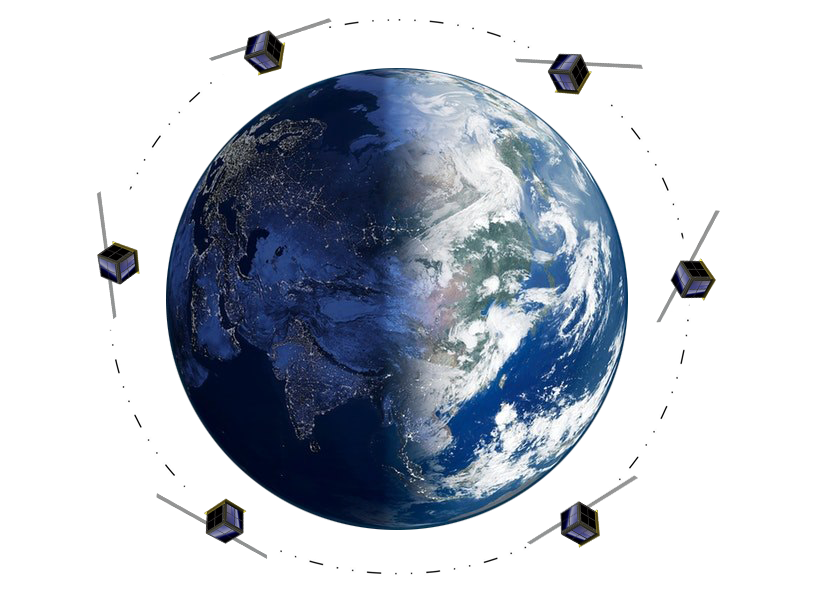
\includegraphics[width=0.8\textwidth]{figures/c1}
\label{fig:forside}
\end{figure}
  \vspace{0.6 cm}
  \begin{center}
%    {\large
%      2. Semester Project Report %Insert document type (e.g., Project Report)
%    }\\
    \vspace{0.2cm}
    {\Large
      Group 18gr1033 %Insert your group name or real names here
    }
  \end{center}
  \begin{center}
  Aalborg University\\
  Control \& Automation\\
  Fredrik Bajers Vej 7\\
  DK-9220 Aalborg
  \end{center}
\end{titlepage}

\clearpage	%frontpage doh
\cleardoublepage
%\begin{document} 
%\thispagestyle{empty}
%\begin{titlepage}
\begin{nopagebreak}
{\samepage 

\begin{tabular}{r}
\parbox{\textwidth}{  \raisebox{-15mm}{
\includegraphics[height=3cm]{figures/aaulogo-en.png}}
\hfill \hspace{2cm} \parbox{8cm}{\begin{tabular}{l} %4.90
{\small \textbf{\textcolor{aaublue}{\colorbox{white}{10\textsuperscript{th} Semester, Project}}}}\\
{\small \textbf{\textcolor{aaublue}{Technical Faculty of IT and Design}}}\\
{\small \textbf{\textcolor{aaublue}{Department of
	Electronics Systems}}}\\ 
{\small \textbf{\textcolor{aaublue}{Control and Automation}}}\\
{\small \textcolor{aaublue}{Fredrik Bajers Vej 7C}} \\
{\small \textcolor{aaublue}{9220 Aalborg}} \\
{\small \textcolor{aaublue}{\emph{en.aau.dk/education/master/control-automation}}}
\end{tabular}}}
\end{tabular}

\begin{tabular}{cc}
\parbox{7cm}{

\textbf{Title:}

Fault Tolerant Attitude Control of a Pico-Satellite Equipped with Reaction Wheels
and Magnetorquers \\ %\fxnote{Input project title}\\

\textbf{Theme:}

\small{
 Master thesis\\
}


\parbox{8cm}{


\textbf{Project Period:}\\
P10, Spring 2018\\
01/02/2018 - 07/06/2018\\
   
\textbf{Project Group:}\\
18gr1033\\ %\fxnote{Input group number}
  
\textbf{Participants:}\\
- Dániel Bolgár  \\
- Nikolaos Biniakos\\
- Alexandru-Cosmin Nicolae\\

\textbf{Supervisors:}\\
Jesper Abilgaard Larsen \\ %\fxnote{Input supervisor}
}\\


\textbf{Pages:} \\
\textbf{Appendices:} 2 (4 pages)\\
\textbf{Attached:} 1 zip file\\
\textbf{Concluded:} 07/06/2018\\

\vfill } &
\parbox{7cm}{
  \vspace{.15cm}
  \hfill
  \begin{tabular}{l}
  {\textbf{Synopsis}}\bigskip \\
  \fbox{
    \parbox{6.5cm}{\bigskip
     {\vfill{\small This report describes the design and simulation of a control system on a AAU-CubeSat, which is a pico- satellite used for Low Earth Orbit flight.

The objective is to use a flight formation for monitoring Greenland, by having eight satellites equally distributed in orbit.

Two controllers must be designed, one to control the angle between the satellites using the drag force, and one for attitude control.  The drag force applied on the satellite depends on the cross section area which can be controlled using the orientation of the satellite.

A linear and a non-linear control method have been designed in order to compare the differences between them.  
     \bigskip}}
     }}
   \end{tabular}}
\end{tabular}} %\vspace{1cm}



\end{nopagebreak}
%\end{titlepage}
%\end{document}
\cleardoublepage
\chapter*{Preface}
This report has been written by group 1033 during fourth semester in Control and Automation MSc in Aalborg University, Department of Electronic Systems during the period from February 2018 to June 2018. It is written as a Master's thesis for the Control and Automation Master's program. 

A nomenclature is included presenting the acronyms, symbols and terminology used throughout the thesis.  Quotes are inside quotation marks and are cursive.

The authors would like to thank Associate Professor Jesper Abilgaard Larsen for supervising. The authors furthermore would like to thank the students involved in the development of the AAUSAT Simulink Library.

% References made before a full stop regards the sentence and reference after full stop regards the paragraph.
Attached to report is a zip file with:
\begin{itemize}
	\item The MATLAB code 
	\item Simulink models
\end{itemize}
\vspace{2cm}

\textbf{Report by:}\\
\vspace{-5pt}
\begin{table}[H]
	\centering
	\begin{tabular}{c c c}
		\underline{\phantom{JAERJAERJAERJAERGO}} & \phantom{cookies} & \underline{\phantom{JAERJAERJAERJAERGO}} \\
		 	Dániel Bolgár	& \phantom{cookies} &  Nikolaos Biniakos	\\
		&&\\
		\multicolumn{3}{c}{\underline{\phantom{JAERJAERJAERJAERGO}}}\\
		\multicolumn{3}{c}{Alexandru-Cosmin Nicolae}\\				
						
	\end{tabular}
\end{table}


\pagebreak


\tableofcontents         %     weath2 er or not you want to create it.
\cleardoublepage

\pagenumbering{arabic} %use arabic page numbering in the mainmatter
\fancyfoot[RO,LE]{\thepage \text{ of} \pageref{LastPage}}
\fancyfoot[RE,LO]{17gr834}
\fancyhead[RE,LO]{}
\fancyhead[RE,LO]{\color{aaublue}\small\nouppercase\leftmark} %even page - chapter title
\pagestyle{fancy}

%||||||||||||||||||||||||||||||||||||||||||||||||||||||||||||||||
%|||||||       Set Section and chapters as input below   ||||||||
%||||||||||||||||||||||||||||||||||||||||||||||||||||||||||||||||

\listoftodos
\printglossary
\printnomenclature 
\chapter{Introduction}\label{chap:Introduction}

Satellites are no longer the privilege of just a handful of economic powerhouses such as nations or mega companies. While the satellites themselves can be engineered to be relatively cheap, there is no avoiding the high cost of putting the satellite into orbit. Many efforts were made recently to reduce this cost. The cost is highly dependent on the weight of the satellite, thus by minimizing the weight 

\section{Problem statement}

\newglossaryentry{AAUSAT}{name={AAUSAT},description={Cool-ass picosatellite}}

\section{Use-case}\label{sec:useCase}



\chapter{System Description}\label{chap:systemDescribtion}

\section{Reaction Wheels}

One method of controlling a spacecraft's attitude is by using either reaction or momentum wheels attached to the spacecraft's body. By controlling the wheel's angular velocity using a motor, the amount of angular momentum stored in the wheel can be controlled. If there are no external forces involved, the sum of angular momentum in the system made up by the spacecraft's body and the reaction wheels is constant. This means that by increasing the angular velocity of the wheels, the satellite body's angular momentum can be reduced. This angular momentum transfer can be used to control the attitude of the satellite. If the goal is to change the angular momentum of the whole satellite, actuators that have external interaction should be used, such as magnetorquers or solar sails.

The difference between momentum and reaction wheels is that the nominal angular velocity of momentum wheels is high in order to store angular momentum, and in the case of reaction wheels, low. Many momentum wheels still turn at an angular velocity larger than zero in order to avoid static friction in the bearings. Reaction wheels usually make up only a small fraction of a satellite's weight. They rely on being able to run at high speeds, making their angular momentum significant. The small weight ratio makes precise controlling easier.


%One design consideration for reaction wheels is maximizing moment of inertia for unit weight. This is done by distributing most of the material near the outskirts of the wheel. There is a trade-off between having most of the mass at the outskirts and durability at high angular velocities. 


Reaction wheels have an angular velocity limitation. This means that if a reaction wheel reaches its maximum angular velocity, it can no longer generate a torque on the satellite's body in one direction. In this scenario the system's controllability decreases, thus it should be avoided. An angular momentum unloading strategy should be designed to avoid it. Instead of returning the angular momentum to the satellite's body, unloading the angular momentum through other methods is preferred. Magnetorquers can be used for such purposes.

Moving parts are usually prone to failures. Reaction wheels are expected to run at high angular velocities, which wears down the lubrication and the bearings. Reaction wheels equipped with active magnetic bearings are in development \cite{MagneticReactWheel}. These can eliminate friction from the system and by controlling the bearing, can even reduce micro-vibrations, increasing the durability of the system. AAUSAT-II itself however uses mechanical wheel bearings.

\subsection{Reaction Wheel Configuration}

There have been studies on what is the best configuration of redundant reaction wheels. The optimal configuration can of course depend on the requirements. In some configurations the   Minimizing energy consumption is normally the goal in deciding on a configuration. Ismail et al. \cite{ReactionWheelConfigSim} investigated several configurations by running simulations with the configuration being the only difference.

evenly distributed

angular acceleration demand \cite{ReactionWheelConfigSim} \cite{reactionWheelConfigThesis}

gps orientation, Earth station

Tetrahedron configuration can output twice as much force along an axis as one wheel can produce along its own axis.

\subsubsection{Transformation Between Body \& Reaction Wheel Space}

The main attitude controller sends torque demands to the actuators. The torque demand distributed to the reaction wheels have to be converted to torques parallel to reaction wheel axes, in order for the motor controllers to function. Transformation from reaction wheel space to body frame is quite intuitive. Knowing the orientation of each motor axis and the corresponding motor torque

\begin{equation}
N_{rw} = A N_{motor} = \begin{bmatrix}
Axis_{1}       & Axis_{2}  & Axis_{3}  & Axis_{4} 
\end{bmatrix} N_{motor}
\end{equation}

\begin{equation}
A N_{motor}  = 
\begin{bmatrix}
\cos(19.47)       & -\cos(19.47) \cos(60)  &  -\cos(19.47) \cos(60)  & 0 \\
0       & \cos(19.47) \cos(30)  &  -\cos(19.47) \cos(30)  & 0 \\
-\sin(19.47)       & -\sin(19.47)   &  -\sin(19.47)   & 1
\end{bmatrix} N_{motor}
\end{equation}

Since $A$ is a $ 4 \times 3 $ matrix, a pseudo inverse has to be used when reordering the equation.

\begin{equation}
N_{motor} = A ^\dagger N_{rw}   =  A^T  (A A ^T)^{-1} N_{rw}
\end{equation}

\nomenclature{$N_{motor$}}{$4\times1 vector where each entry represents the torque of each reaction wheel motor. $}

\cite[equation 18.41-42]{SADC}
\cite{reactionWheelConfigThesis}

\begin{equation}
h_{rot} = A\left[ h_1, h_2, h_3, h_4 \right]^T
\end{equation}

\begin{equation}
N = A^R \textbf{$N_rw$} + k\left(1,-1,-1,1\right)
\end{equation}

\todo{revise 2nd part}

The torque demand for the satellite's body

\subsubsection{Reconfiguration}

Fault isolation for the redundant reaction wheel configuration can be done by detecting which is the reaction wheel where the fault occurred and shutting it off and redistributing the torques to the rest of the reaction wheels. This reconfiguration can be represented by swapping the corresponding faulty columns to zero vectors. For example, if a fault occurs in the 3rd reaction wheel:

\begin{equation}
A_{f3} = \begin{bmatrix}
Axis_{1}       & Axis_{2}  & 0  & Axis_{4} 
\end{bmatrix}
\end{equation}

The pseudo inverse is calculated in the same manner as presented in ... 

\section*{Magnetorquer model}
\nomenclature[Sncoil]{$n_{coil}$}{The number of windings of the coil}
\nomenclature[SIcoil]{$I_{coil}$}{The electric current flowing through the coil}
\nomenclature[SAcoil]{$\vec A_{coil}$}{The vector perpendicular to the cross-sectional area of the magnetorquer}
\nomenclature[Sm]{$\vec m_{mt}$}{The magnetic dipole moment}

Since the primary actuators for the satellite are chosen to be reaction wheels, four magnetorquer will be used for desaturation of the reaction wheels.  

Having a solenoid onboard of the satellite, referred as a magnetorquer through which the current could be controlled and hence the dipole moment.

The interaction of the dipole with the magnetic field of the Earth will result in a torque that will be perpendicular to the magnetic field vector according to the following equation \cite{SADC}:
\begin{flalign}
   \vec N_{mt} = \vec m_{mt} \times \vec B
	\label{eq:NT}
\end{flalign} 
where $\vec N$ is the torque produce by the magnetorquer and will be the torque that will influence the satellite dynamics, $\vec B$ is the vector of the magnetic field of the Earth and $\vec m_{mt} $ is the magnetic dipole moment generated by the magnetorquer.

The magnetic moment $\vec m_{mt}$ is given by \cite{MagMom}:
\begin{flalign}
	\vec m_{mt} = n_{coil} \ I_{coil} \ \vec A_{coil}
	\label{eq:mm}
\end{flalign} 
where $n_{coil}$ is the windings of the coil, $I_{coil}$ is the electric current on the coil and $\vec A_{coil}$ is the vector perpendicular to the cross-sectional area of the magnetorquer.

Using \ref{eq:NT} and \ref{eq:mm} and taking the magnitude, the applied torque on the satellite is \cite{SJ}:
\begin{flalign}
	\vec N_{mt} = n_{coil} \ \rvert I_{coil}\rvert \ \rvert \vec A_{coil}\rvert \ |\vec B| \sin (\theta)
	\label{eq:ft}
\end{flalign} 
where $\sin (\theta)$ is the angle between the plane $A_{coil}$ and the magnetic field vector $\vec B$.

Furthermore, the resistance of the magnetorqer which is a function of the temperature of the coil given as an input, can be computed as
\begin{flalign}
R_{mt} = \dfrac{nC  \rho_{mt} }{A_{wire}} = \dfrac{nC \rho_0(1+\alpha_0(T_{mt} - T_0))}{A_{wire}}
\label{eq:rt}
\end{flalign} 
where \\
$R_{mt}$ is the resistance of the magnetorquer \\
$n$ is the number of windings \\ 
$C$ is the wire circumference  \\
$A_{wire}$ is the wire cross-sectional area  \\
$\rho_0$ is the resistivity of copper  \\
$\alpha_0$ is the coefficient of resistivity temperature   \\
$T_{mt}$ is the temperature given as an input   \\
$T_0$ is the resistivity base temperature  

Using the computed resistance the current is found by dividing the voltage by the resistance of the magnetorquer. Next, in order to find the magnetic moment $m$, the current is multiplied by the number of windings and the area of the wire. For finding the torque that acts on the satellite, the magnetic moment is multiplied by the coil normal and a cross-product is used between this multiplication and the magnetic field of the Earth.

In order to find what voltage to output for having a certain amount of torque, a gain between voltage and magnetic moment is found. For the coil model, the control signal is the voltage. Therefore, translating the magnetic moment demand to voltage is found as follows:
\begin{flalign}
\frac{\vec m_{mt}}{v} = \frac{n_{coil} \vec A_{coil} \vec I_{coil}}{R_{mt}} \mathcal {K}
	\label{eq:gain}
\end{flalign} 
\begin{flalign}
 \mathcal{K} = \frac{\vec m_{mt} R_{mt} }{ n_{coil}  \vec A_{coil} \vec I_{coil} v}
	\label{eq:gainn}
\end{flalign} 
where \\
$v$ is the voltage \\
$\mathcal {K}$ is the gain

The voltage can be found using the following transfer function:
\begin{flalign}
	\frac{I_{coil}}{v} = \frac{1}{R_{mt}}
	\label{eq:voltage}
\end{flalign} 

where the voltage is found to be $1.25 V$

Given a current $I$ going through a coil, the interest is to find the magnetic field $B$ at a certain point located distance $r$ from the coil. Finding an estimate of the magnetic field at any point will give the possibility to change the location of the magnetometers around. For computing the magnetic field in the center of a rectangular coil, the law of Biot-Savart is used \cite{SJ}:
\begin{flalign}
	d\vec B = \frac{\mu_0 I}{4 \pi}  \frac{d \vec s \times \hat{\vec r}}{r^2}
	\label{eq:BS}
\end{flalign} 
where \\
$\vec B$ is the magnetic field \\
$\mu_0$ is a constant called permeability of free space and is equal with $4\pi \times 10^{-7}  \ Tm/A$ \\
$I$ is the current \\
$d \vec s $ is a length element in the direction of current \\
$\hat{\vec r}$ is the direction from $d \vec s$ to a particular position \\
$r$ is the distance from $d \vec s$ to a particular position

The magnetic field $B$ at any point is directly proportional to the current $I$ that is crossing the coil. The magnetic field generated by the current from equation \ref{eq:BS} is just a small length element $d \vec s$ of the coil. For finding the total magnetic field, all small elements need to be summed up and for this the magnetic field $B$ have to be evaluated by integrating equation \ref{eq:BS}.

The design of the magnetorquer is described in appendix \ref{chap:F}.


\chapter{Requirements}\label{chap:requirements}
Based on the use-case introduced and the available system a set of requirements are formulated.
%
\subsection*{System requirements}
%
\begin{enumerate}
	\item \textbf{The satellite should reconfig scheme control .}
	
	desc
	
	\item \textbf{The satellite should detect the faults .}
	
	desc
	
\end{enumerate}

The satellite shall detect certain actuator faults.

It should be able to reconfigure the control scheme in order to handle faults. 



MUST is equivalent to REQUIRED and SHALL indicating that the definition is an absolute requirement.

MUST NOT is equivalent to SHALL NOT and indicates that it is an absolute prohibition of the specs.

SHOULD is equivalent to RECOMMENDED means that there are valid reasons to ignore a particular requirement, but the implications need to be weighed.

SHOULD NOT and NOT RECOMMENDED means that a particular behavior may be acceptable or useful, but again, the implications need to be weighed.

MAY means OPTIONAL and that the requirement is truly optional. Interoperability with different systems that may or may not implement an optional requirement must be done.

$\dot \omega $
\chapter{Satellite Modeling}
\todo{maybe some intro}
\section{Reference Frames}

\nomenclature[A]{\textbf{ECI}}{Earth Centered Inertial Frame}
\nomenclature[A]{\textbf{ECEF}}{Earth Centered Earth Fixed Frame}
\nomenclature[A]{\textbf{SBRF}}{Satellite Body Reference Frame}

Using different reference frame for different calculations can simplify equations. Values in one reference frame can be converted into the other by using the proper transformations.
Inertial frames of reference are frames where Newton's 3 laws of dynamics apply.
The most used reference frames for Earth-orbiting satellites are Earth Centered Inertial Frame (ECI), Earth Centered Earth Fixed Frame (ECEF), Orbit Frame, Satellite Body Reference Frame (SBRF)  \cite{ref1} \cite{ref2}. Figure \ref{fig:frames} provides a visualization of the frames.

\begin{figure}[h!]
	\centering 
	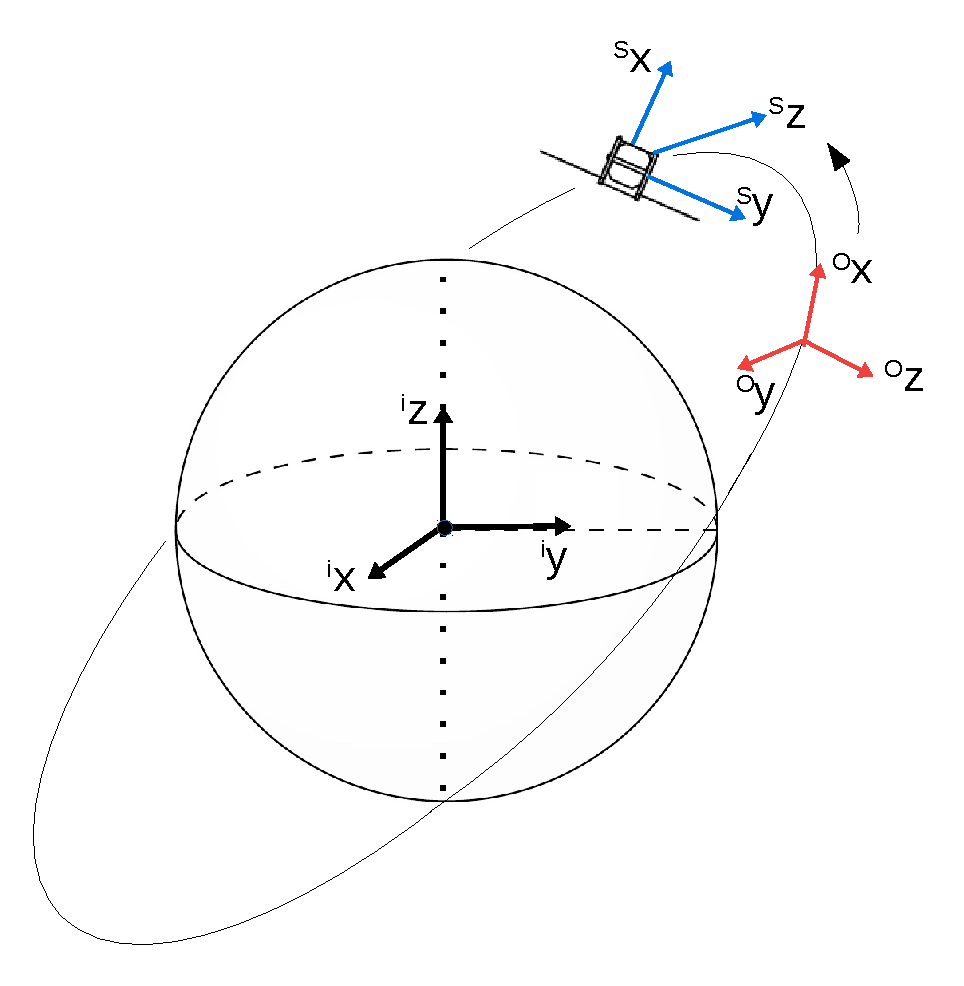
\includegraphics[width=140mm]{figures/frame.pdf}	
	\caption{Reference frame axes. Superscripts: i - ECI, o - Orbital, s - Satellite Body Frame \cite{our_report}.}
	\label{fig:frames}
\end{figure}

\subsubsection{Earth Centered Inertial Frame (ECI)}
Earth is rotating and is orbiting the Sun, it accelerates in the direction of the Sun's center of mass, the Sun is orbiting the center of the Milky Way, etc. Thus there is no frame fixed to Earth's center that is an inertial frame \textit{per definitionem}. But in the case of earth orbiting satellites, there exists a coordinate system attached to Earth's center that out of practical considerations can be treated as one, the Earth Centered Inertial Frame (ECI).
As the name suggests, the origin of the coordinate system is the center of earth. Inertial means that the frame doesn't rotate, the direction of stars remain the same. 
ECI is a cartesian coordinate system. Its $^iz$ vector points in the direction of the northern axis of rotation, while the $^ix$ axis towards the vernal equinox. The $^iy$ axis completes the triad of the right-handed Cartesian coordinate system.


\nomenclature[T]{\textbf{Vernal Equinox}}{The vernal equinox is the vector pointing towards the Sun's center during the equinox (20th of March in 2018). The $x$ vector also keeps its direction relative to the stars.}


\subsubsection{Earth Centered Earth Fixed Frame (ECEF)}

ECEF, similarly to ECI is centered at the Earth's origin. Its $z$ vector points towards the north parallel to the rotational axis. Its $x$ axis points at $0\deg$ latitude and $0\deg$ longitude on the Earth's surface, thus following Earth's rotation. This makes ECEF non-inertial. $y$ axis completes the right-handed triad.

\subsubsection{Orbital Frame}

The Orbital Frame is centered at the center of mass of the satellite. The $^oz$ axis points towards the center of Earth, $^ox$ points in the direction of the satellite's velocity, while $^oy$ is the normal vector for the orbital plane. The 3 axes make up an orthogonal triad.

\nomenclature[T]{\textbf{Nadir}}{The axis pointing towards Earth's center of mass}

\subsubsection{Satellite Body Reference Frame (SBRF)}

Body-fixed frames are attached to the satellite's body, but the orientation of the frame in relation to the body is arbitrary. Due to practical considerations the axes of the SBRF are chosen to line up with the principal axes of inertia of the body.

\section{Satellite equations of motion }
The satellite equations of motion is split into a kinematic model, which will describe the relation between the orientation of the satellite and the time derivative of the orientation using the rotation of the ECI and SBRF frame, while a dynamic model is established in order to relate the disturbance torques which influence the satellite and the angular velocity.

The derivation of the satellite equations of motion is presented in appendix \ref{chap:C}, therefore, putting together both dynamic and kinematic equation derived in the appendix, the system equations of the satellite will be non-linear and can be combined into a state-space representation as follows:
\begin{flalign}
	\begin{bmatrix}
		\vec{ ^s_i\dot q(t)} \\
		\vec{\dot \omega{(t)}}
	\end{bmatrix} 	
	= 
	\begin{bmatrix}
		\frac{1}{2} \underline{ \Omega}_{(4\times4)} \vec{ ^s_i q(t)} \\
		{-\underline{I}_{s}^{-1}\underline{S}(\vec{\omega})\underline{I}_{s}\vec{\omega}(t)-\underline{I}_{s}^{-1}\underline{S}(\vec{\omega})\vec{h_{rw}}-\underline{I}_{s}^{-1}\vec{N_{rw}}(t)+\underline{I}_{s}^{-1}[\vec{N_{mt}(t)}+\vec{N_{dis}}(t)}]
	\end{bmatrix} 
	\label{eq:seom}
\end{flalign}
where,\\
$\vec{ ^s_i  q(t)} = [q_1 \ q_2 \ q_3 \ q_4]^T$ \\
$\vec{\omega{(t)}} = [ \omega_1 \ \omega_2 \ \omega_3]^T$ \\
$\underline{\Omega}(\omega)$ is the $4\times4$ skew symmetric matrix \\
$\underline{I}_{s}$ is the inertia matrix \\
$\underline{S}(\omega)$ is the $3\times3$ skew symmetric matrix \\
$\vec{N_{dis}}(t)$ is the disturbance torque \\
$\vec{N_{rw}}$ is the torque from momentum wheels \\
$\vec{N_{mt}}$ is the torque from magnetorquers  \\
\subsection{Linearized equation of motion}
For the purpose of designing a linear controller, the equations of motion of the satellite need to be linearized. The whole process of linearization is presented in appendix \ref{chap:C}.

Therefore, by using the results from appendix \ref{chap:C} the linear equation of motion can be combined in a state-space form as:
\begin{flalign}
	\begin{bmatrix}
		\vec{ \dot {\tilde{^s_iq}}(t) } \\
		\vec{ \dot {\tilde{\omega}}(t) }
	\end{bmatrix} 	
	= 
	\begin{bmatrix}
		-\underline{S}(\vec{\bar{\omega}}) &	\frac{1}{2} \underline{\vec 1}_{(3\times3)} \\
		\underline{ 0}_{(3\times3)} &	{\underline{I}_{s}^{-1}\underline{S}(\underline{I}_{s}\vec{\bar{\omega}})-\underline{I}_{s}^{-1}\underline{S}(\vec{\bar{\omega}})\underline{I}_{s}}
	\end{bmatrix} 
	\begin{bmatrix}
		\vec{  {\tilde{q}}(t) } \\
		{  {\tilde{\vec \omega}}(t) }
	\end{bmatrix} 	
	-
	\begin{bmatrix}
		\underline{\vec 0}_{(3\times3)} \\
		{\underline I_{s}^{-1}}
	\end{bmatrix} 	
	\vec {\tilde N_{ctrl}}
	\label{eq:lele}
\end{flalign}
where,
$\vec{\tilde N_{ctrl}}$ is the torque from magnetorquers and the reaction wheels and is defined as $\vec{\tilde N_{ctrl}} = \vec{N_{mt}} - \vec{N_{rw}}$. \\
\section {Environmental disturbance torques}
  \label{chap:distTorques}
%
Disturbance torques can be classified either as external or internal \todo{don't distinguish between external and internal}. Since the external disturbances are larger in magnitude compared to \todo{reference} internal and can cause a change in the total momentum of the spacecraft, only these will be accounted. The external disturbing torques that will be discussed are aerodynamic, solar radiation and gravity gradient torque.
\subsection*{Aerodynamic disturbance torque}\label{chap:disturbances}
%
Gas molecules, in a LEO(low Earth orbit) collide with the surface of the satellite causing
a force which direction opposes the direction of the satellites velocity vector. This Aerodynamic force can be modelled as \cite{SADC,our_report}  


\begin{flalign}
	\vec{F_A} = -\frac{1}{2} \rho \ C_D \ A_{\perp}   \vec{v}^2
	\label{eq:ec1c}
\end{flalign}

where $\rho$ is the atmospheric density  
is chosen to be constant and equal to $1.454 \cdot 10^{-13} Kg/{m^3}$ based on the Committee on Space Research\cite{FSA}, $\vec{v}$ is the satellite velocity vector, $A_{\perp}$ is the area perpendicular to the velocity and $C_D$ is the drag coefficient and is usually chosen to be equal to 2 \cite{SADC}\cite{our_report}  . If the calculation of the lifetime of the satellite is of great importance a more accurate drag coefficient should be used.

\begin{figure}[h!]
	\centering
	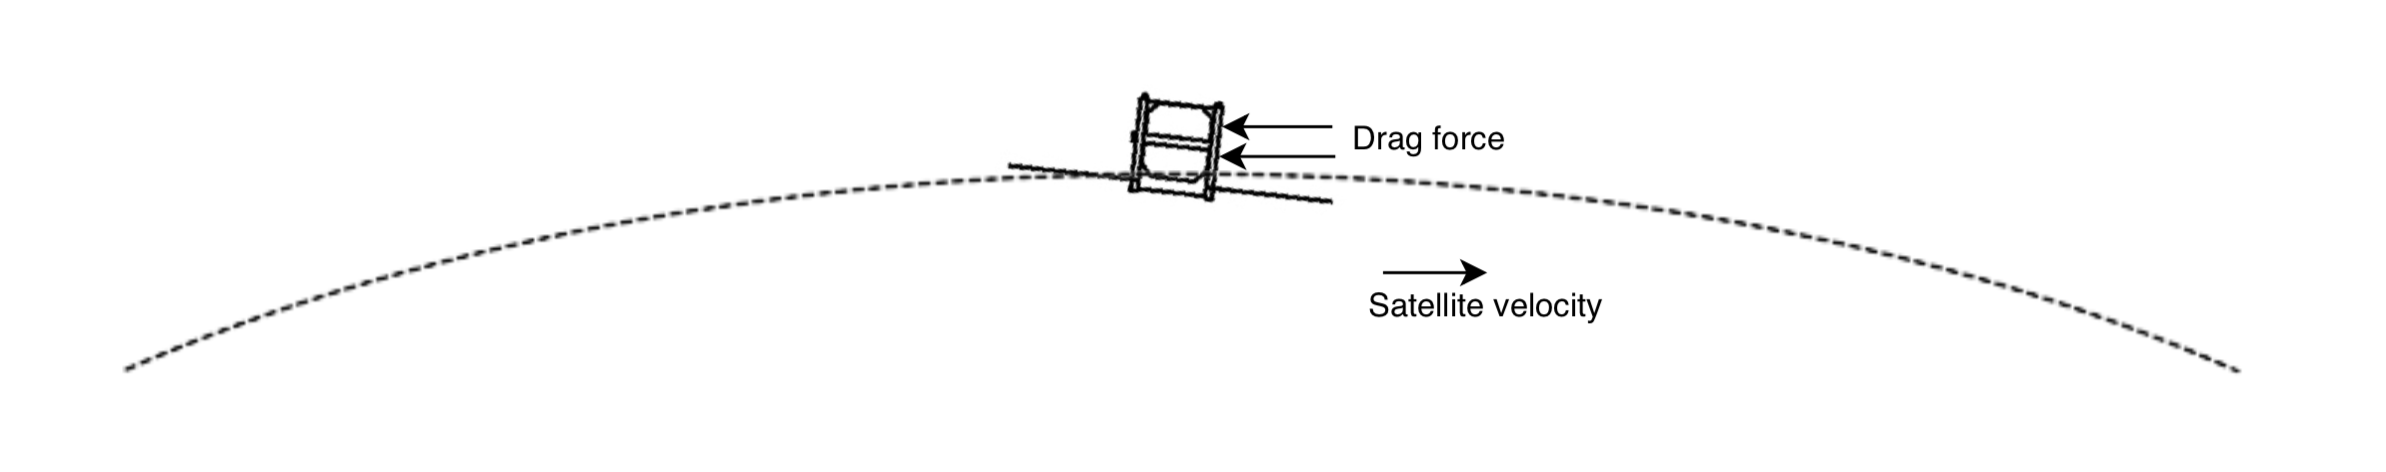
\includegraphics[width=0.9\linewidth]{figures/AFF}
	\caption{Aerodynamic disturbance force actiong on the satellite on orbit}
	\label{fig:af}
\end{figure}

Using the \eqref{eq:ec1c}, the aerodynamic torque acting on the satellite can be written as 
\begin{flalign}
	\vec N_{drag} = \vec r_{s} \times  \vec F_{A} 
	\label{eq:drag}
\end{flalign}
where:\\
$\vec r_{s}$ is the vector from the centre of mass of the satellite to the geometric centre of the exposed area

\subsection*{Solar radiation disturbance torque}\label{chap: disturbances2}

Solar radiation pressure is emitted from various sources such as reflection from the Earth's atmosphere, from solar wind and direct radiation from the sun to the surface of the satellite\cite{SADC}\cite{our_report}  . Direct radiation is larger and only this source will be taken into account.

\begin{table}[H]
	\begin{minipage}[b]{0.49\linewidth}
		\centering
		\begin{figure}[H]
			\centering
			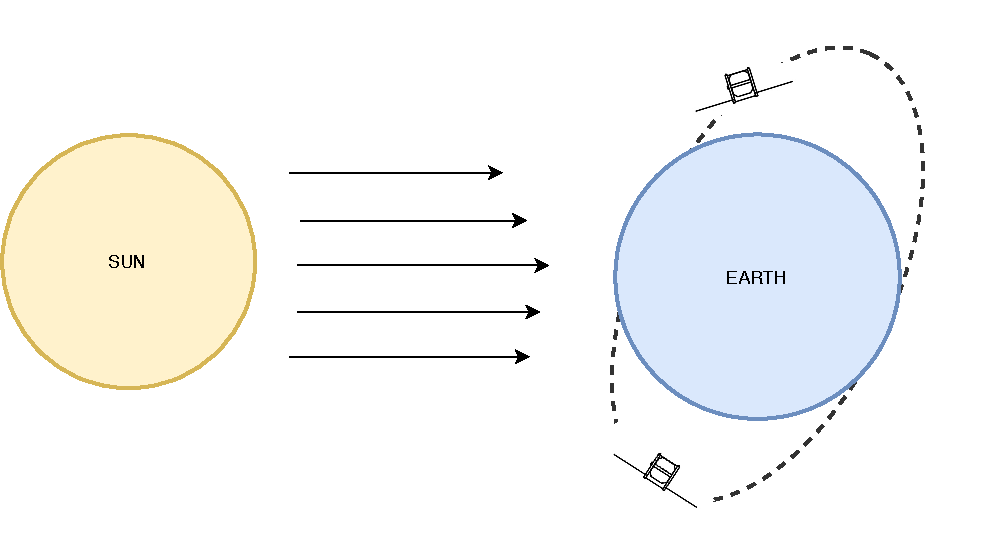
\includegraphics[width=1\linewidth]{figures/sunRAD}
		
		\end{figure}
	\end{minipage}\hfill
	\begin{minipage}[b]{0.49\linewidth}
		\centering
		\begin{figure}[H]
			\centering
			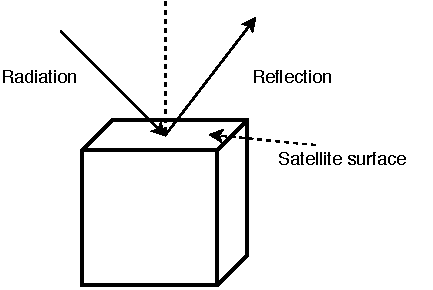
\includegraphics[width=0.55\linewidth]{figures/solarRad}
		
		\end{figure}
	\end{minipage}
	\caption{ Sun radiation actiong on satellite surface}
	\label{fig:radf}
\end{table}

The solar flux is given as
\begin{flalign}
	P = \dfrac{F_s}{c}
	\label{eq:flux2}
\end{flalign}

where $F_s$ is the intensity or mean energy flux given as 1358 [$W/m^2$] and $c$ is the speed of light. The solar radiation force $\vec F_{rad}$ can be expressed as 

\begin{flalign}
	\vec {F_{rad}} = C_{a} P A \ \hat{S}
	\label{eq:Pres}
\end{flalign}
where $C_{a}\in [0,2]$ is the absorption coefficient which depends on the material of the satellite with 2 \todo{decide if 1.5 or 2 should be used} be the value of totally reflected beam, $P$ is the solar flux, $A$ is the radiated surface area, and $\hat{S} =\frac{\vec {r_{sun,sat}}}{||\vec {r_{sun,sat}}||}$ is the unit vector from the satellite to the sun. The solar radiation torque can be computed as 
\begin{flalign}
	\vec N_{solar} = \vec r_{s} \times  \vec F_{rad} 
	\label{eq:solar}
\end{flalign}
where $\vec r_{s}$ is the vector from the center of mass of the satellite to the center of pressure.
%
\subsection*{Gravity Gradient disturbance torque and $J_2$  perturbation}\label{chap: disturbances3} \todo{separate}
%
Due to the non spherical mass distribution and non homogeneity of the Earth, a pertubative gravitational force($J_{2}$ perturbation)\cite{SADC}\cite{our_report} exerted on the satellite determining its orbit difference compared to ideal mathematical models.
Contrary to this, in order to derive an expression for the gravitational torque exerted about the mass centre of the satellite, it will be assumed symmetrical, spherical distribution of the Earth's mass\cite{SADC} with this assumption be valid by comparing the magnitude of the gravity gradient with the other pertubative torques.     
\subsubsection{$J_2$ gravity perturbation}
An approximation of the gravitational potential of the Earth is \cite{SADC}\cite{our_report}:
\begin{flalign}
	U \approx -\frac{\mu}{r} \left[1 - \sum_{n=2}^{\infty} \left(\frac{R_e}{r}\right)^{n} J_n P_n sin(\phi)  \right ] = \frac{\mu}{r} [U_0 + U_{J_2} + U_{J_3} + ...]
	\label{eq:Pr341}
\end{flalign}
which has been derived using the spherical harmonic expansion describing deviations of the potential to the south and north direction,
with $U_0$ = -1, $U_{J_2}$ = $\left(\frac{R_e}{r}\right)^{2} J_2 \frac{1}{2} (3 sin^2 \phi -1) $ and ${J_2}$ be a numerical coefficient, with the other terms been discarded.

The final relation is obtained as 
\begin{flalign}
	\vec F = -m \nabla U
	\label{eq:Pr3431}
\end{flalign}
with the vector $\vec F$ expand to the components \cite{SIDI}\cite{our_report}  :
\begin{flalign}
	F_x = -\frac{\partial U}{\partial x} = \mu \left[ -\frac{x}{r^3} + A_{J_2} \left(15 \frac{xz^2}{r^7} - 3\frac{x}{r^5}   \right ) \right ]       \\
	F_y = -\frac{\partial U}{\partial y} = \mu \left[ -\frac{y}{r^3} + A_{J_2} \left(15 \frac{yz^2}{r^7} - 3\frac{y}{r^5}   \right ) \right ]       \\
	F_z = - \frac{\partial U}{\partial z} =  \mu \left[ -\frac{z}{r^3} + A_{J_2} \left(15 \frac{z^3}{r^7} - 3\frac{z}{r^5}   \right )  \right]       
	\label{eq:Pr34331}
\end{flalign}
where $A_{J_2}  = \frac{1}{2} J_2 R_e^2$ and and $R_e$ is the mean radius o the Earth at the equator
%
%
\subsubsection{Gravity-Gradient torque}
The gravity gradient effect about the centre of mass of the satellite is a consequence of the non uniform gravitational field of the Earth. The torque about the centre of mass of the satellite can be expressed as\cite{SADC}\cite{our_report}  

\nomenclature[A]{\textbf{COM}}{Center of Mass}
%
\begin{flalign}
	\vec N_{gg} &= \dfrac{3\mu}{\vec R_{sc}^3}[\vec{\hat R_{sc}} \times(\vec{I} \ \vec{\hat R_{sc}}] 
	\label{eq:ref4}
\end{flalign}
where $\vec{\hat R_{sc}}$ is the unit vector from geometric centre of the earth's to the satellite's geometric centre, $\mu = G*m_{earth}$ with $G$ be the Gravitational constant $6.6740*10^{-11}$ [$m^{3} kg^{-1} s^{-2}$] and $\underline I$ is the inertia matrix of the satellite. 

\begin{figure}[H]
	\centering
	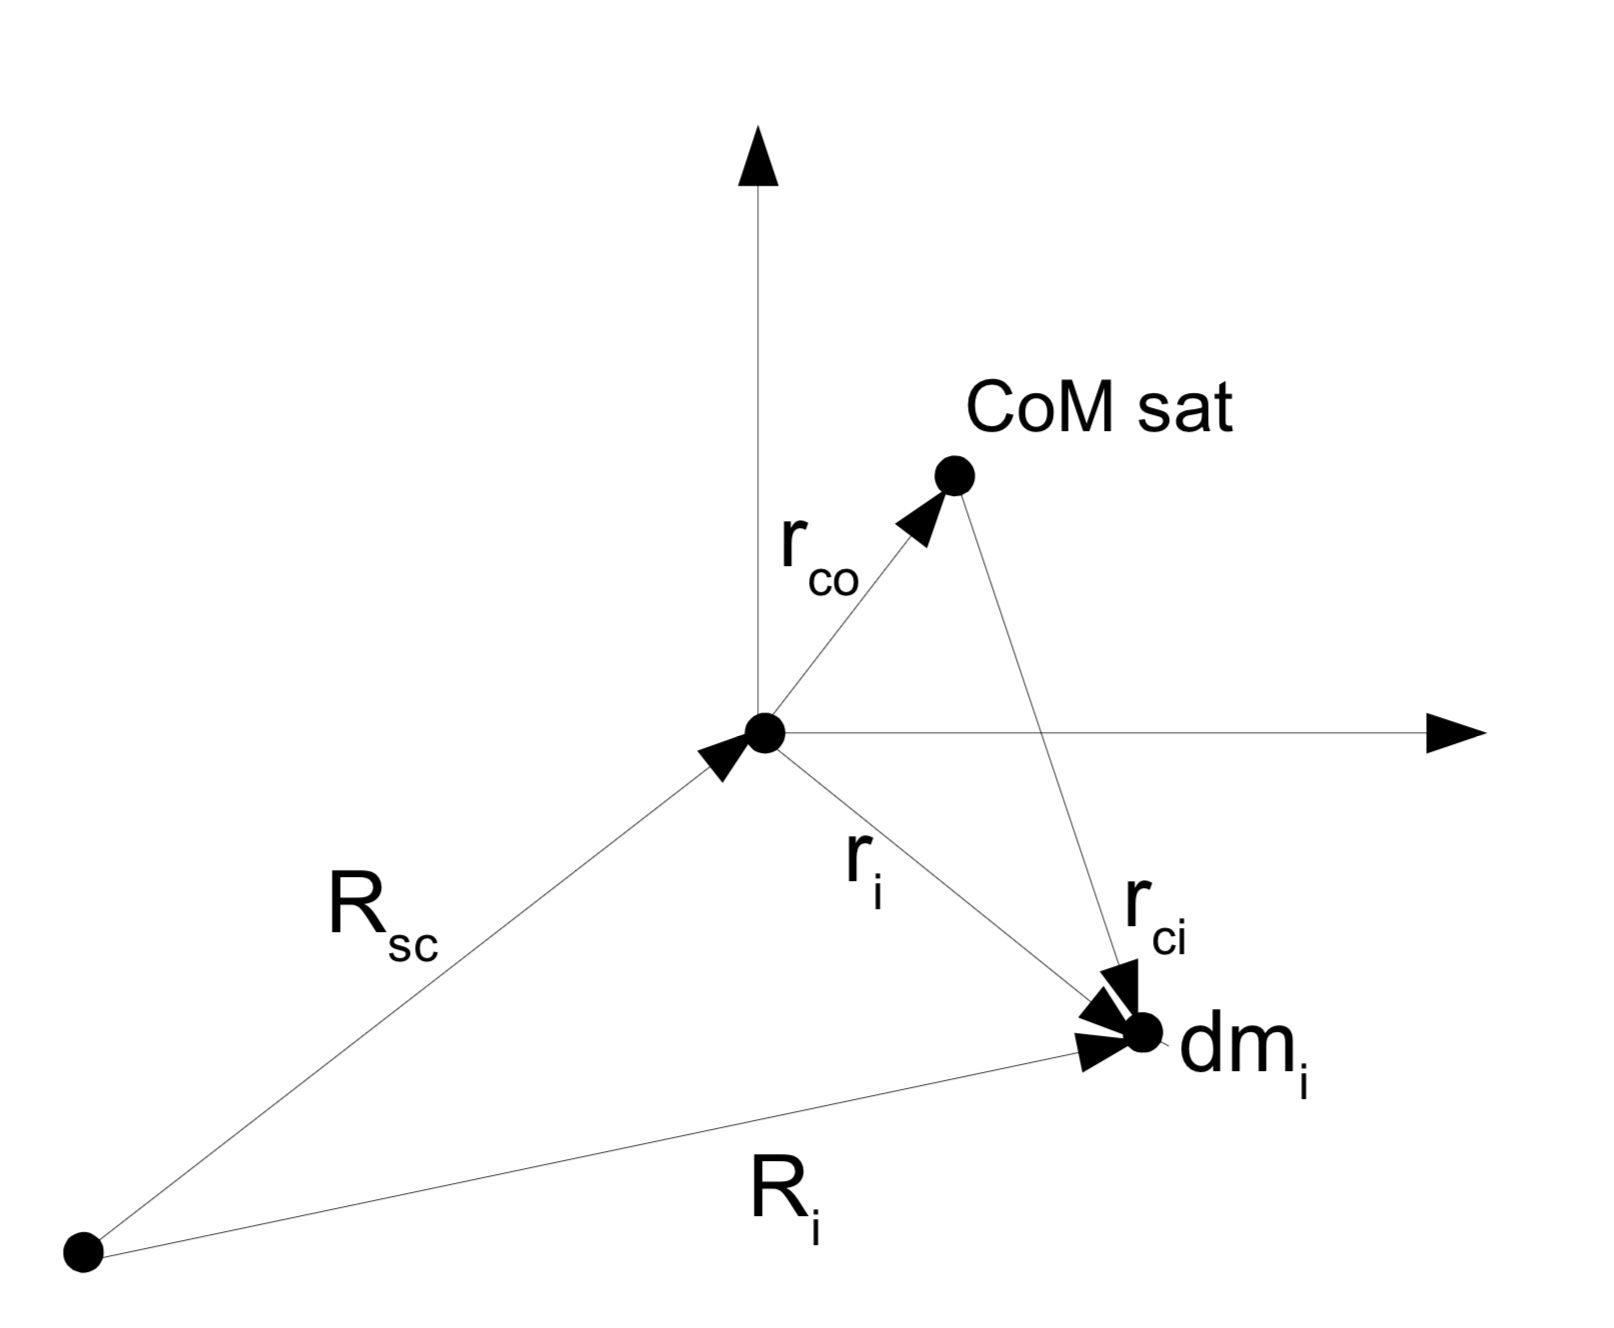
\includegraphics[width=0.5\linewidth]{figures/ggt}
	\caption{Gravity gradient torque computation using the coordinate system}
	\label{fig:gg}
\end{figure}

\subsection{Magnetic residual }
When the satellite orbits the Earth, due to the interference of the magnetic field of the Earth and the satellite magnetic residual, an extra disturbance torque is generated. Because the satellite can not be perfectly isolated, the actuators and sensors will produce a residual magnetic moment. Similarly like magnetorqers, the torque generated by the magnetic residual can be computed using:
\begin{flalign}
\vec N_{mr} = \vec m \times \vec B
\label{eq:st}
\end{flalign}
where $\vec m$ is the magnetic moment and $\vec B$ is the magnetic field of the Earth.

The magnetic field of the Earth can be approximated using \cite{SMAD}:
\begin{flalign}
B = \dfrac{2M}{R^3}
\label{eq:ftf}
\end{flalign}
where $M$ is the Earth magnetic moment and $R$ is the distance from the Earth to the center of the satellite.

\nomenclature[SNmr]{$\vec N_{mr}$}{The torque generated by the magnetic residual }
\nomenclature[Smr]{$\vec m_{mr}$}{The magnetic residual}
\nomenclature[SB]{$\vec B$}{The magnetic field of the Earth}
\nomenclature[SM]{$\vec M$}{The Earth magnetic moment }
\nomenclature[SR]{$\vec R$}{The distance from the Earth to the center of the satellite}
\subsection{Total disturbance torque}
The total disturbance torque acting on the satellite in the SBRF is:

\begin{flalign}
	N_{dist} = N_{drag} + N_{solar} + N_{gg} + N_{mr}
	\label{eq:TDT}
\end{flalign}
\subsection{Reaction Wheel Configuration}
\label{ref:reactConfig}

Studies have been conducted on what is the best configuration of redundant reaction wheels. The optimal configuration can of course depend on the requirements. If the requirement is to have the same controllability for reaction wheels in case of fault, and 6 reaction wheels are available, orthogonally configured double reaction wheels can be used. Minimizing energy consumption is normally the goal in deciding on a configuration. Ismail et al. \cite{ReactionWheelConfigSim} investigated several configurations by running simulations with the configuration being the only difference. The tetrahedron configuration of 4 reaction wheels has been chosen as the default configuration in the present thesis, which is quite widespread in the field \cite{reactConfigNasa}, and is redundant with an excess of one wheel. The tetrahedron configuration is visualized in Figure \ref{fig:tetrahedron}.
In tetrahedron configuration the 4 wheel orientations are evenly distributed, unlike the also widespread pyramid configuration. 

\begin{figure}[H]
	\centering 
	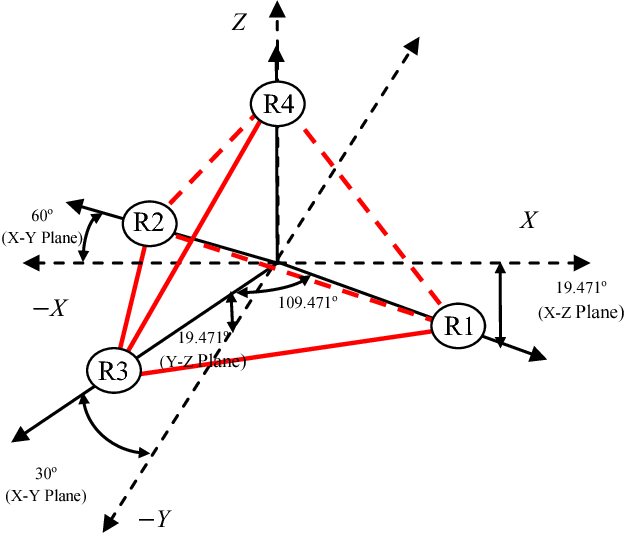
\includegraphics[width=120mm]{figures/tetrahedron}	
	\caption{Geometry of the tetrahedron configuration \cite{Kumar2015DesignAD}}
	\label{fig:tetrahedron}
\end{figure}

%Tetrahedron configuration can output twice as much force along an axis as one wheel can produce along its own axis.
%\cite{reactionWheelConfigThesis} 

\subsubsection{Transformation Between Body \& Reaction Wheel Space}

The main attitude controller sends torque demand signal to the actuators. The reaction wheel torque demand has to be converted from body frame to torques parallel to reaction wheel axes. This transformation is nontrivial. Transforming back from reaction wheel space to body frame is quite intuitive. Knowing the orientation, the mounting angle of each motor axis and the corresponding motor torque, the torque in body frame for tetrahedral configuration can be derived according to equation \ref{eq:motorTrans1} - \ref{eq:transmatrix}. The matrix for tetrahedron configuration is given by \cite{reactionWheelConfigThesis}.

\begin{equation}
\label{eq:motorTrans1}
\vec{N_{rw}} = \underline{A}_{M} \vec{N_{M}} = \begin{bmatrix}
\vec{Axis^{M}_{1}}       & \vec{Axis^{M}_{2}}   & \vec{Axis^{M}_{3}}   & \vec{Axis^{M}_{4}} 
\end{bmatrix} \vec{N_{M}}
\end{equation}

\begin{equation}
\underline{A}_{M} \vec{N_{M}}  = 
\begin{bmatrix}
\cos(19.47)       & -\cos(19.47) \cos(60)  &  -\cos(19.47) \cos(60)  & 0 \\
0       & \cos(19.47) \cos(30)  &  -\cos(19.47) \cos(30)  & 0 \\
-\sin(19.47)       & -\sin(19.47)   &  -\sin(19.47)   & 1
\end{bmatrix} \vec{N_{M}}
\label{eq:transmatrix}
\end{equation}

where $\vec{N_{rw}}$ is the reaction wheel torque in body frame, $\vec{N_{M}}$ is the vector containing the reaction wheel DC motor torques parallel to their axes, $\vec{Axis^{M}_{i}}$ are the reaction wheel motor orientation in body frame, $\underline{A}_{M}$ is the transformation matrix between axis oriented reaction wheel torque and torques in 3 dimensional body frame.

The transformation matrix for orthogonal configuration is quite trivial, and is presented in equation \ref{eq:orthoMatrix}.

\begin{equation}
\underline{A}_{M,orth}  = 
\begin{bmatrix}
1       & 0  &  0 \\
0       & 1  &  0  \\
0       & 0   & 1
\end{bmatrix} 
\label{eq:orthoMatrix}
\end{equation}


\nomenclature[S]{$\vec{N_{rw}}$}{Reaction wheel torque in body frame }
\nomenclature[S]{$\vec{N_{M}}$}{$4\times1$ vector containing the reaction wheel motor motor torques parallel to their axes }
\nomenclature[SAdc]{$\underline{A}_{M}$}{Transformation matrix between axis oriented reaction wheel torque and torques in 3 dimensional body frame }

The nontrivial body frame to motor frame transformation can be derived by reordering equation  \ref{eq:motorTrans1}. Since $\underline{A}_{M} $ is a $ 4 \times 3 $ matrix, a pseudo inverse has to be used when reordering the equation, as presented in equation \ref{eq:motorTrans}. 

\begin{equation}
\label{eq:motorTrans}
\vec{N_{M}} =  \underline{A}_{M} ^\dagger \vec{N_{rw}}   =  \underline{A}_{M}^T  (\underline{A}_{M} \underline{A}_{M} ^T)^{-1} \vec{N_{rw}}
\end{equation}

\begin{figure}[H]
	\centering 
	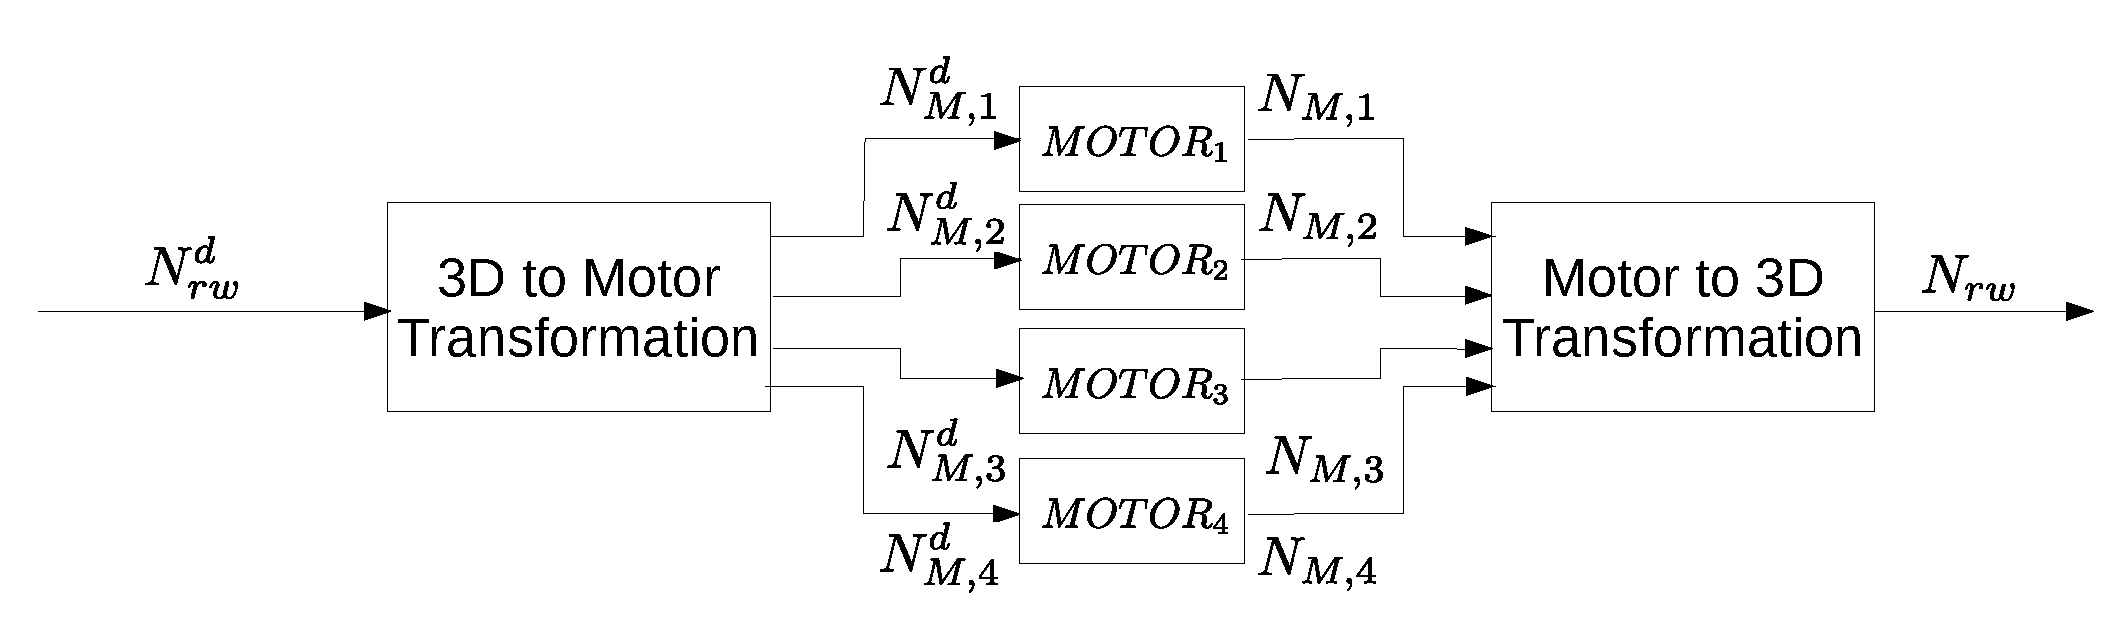
\includegraphics[width=170mm]{figures/distribution}	
	\caption{Reaction wheel torque distribution}
	\label{fig:torqueDistribution}
\end{figure}


%\begin{equation}
%h_{rot} = A\left[ h_1, h_2, h_3, h_4 \right]^T
%\end{equation}

In case there's a demand to adjust the torque distribution between the wheels, an extra vector can be included, as shown in equation \ref{eq:TorqueDistrib}
\cite[equation 18.41-42]{SADC}. If k is set to 0, the norm of wheel torques are minimized.

\begin{equation}
\label{eq:TorqueDistrib}
 \vec{N_{M}} = \underline{A}^\dagger_{M} \vec{N_{rw}}  + k\left[1,-1,-1,1\right]^T
\end{equation}



\chapter{Actuators modelling and control}\label{chap: modeling}
 \textit{This chapter will describe the chosen reaction wheels and BLDC motors along with the electrical and mechanical modelling of the motors.} 
%
\section{Reaction wheels}
%
%Since the focus of the current thesis is not on the design of reaction wheels, only few constraints are  taken into account for the selection of the wheels, such as the weight and the inertia. In order to minimize the total weight of the satellite, the weight of each wheel, is not overcome the %weight of each motor. 

The satellite should be capable of tracking an Earth station in order to be able to downlink data effectively. Tracking a ship requires similar control capability, since the velocity of the wheel is practically zero compared to the velocity of the satellite. Directing the satellite to the nadir continuously only requires keeping a satellite angular velocity equal to the orbit's angular velocity.
Pointing the antennas to the Earth station requires torque from the actuators, the torque demand can be calculated based on the angular acceleration demand for Earth station tracking.
%


 The wheel moment of inertia is \cite{flywheel_design_thesis} $I_{w} = 2.456 [gcm^2]$ and the weight is $m_{w} = 4.201 [g] $ compared to the motor weight $m_{motor} =8 [g] $ and the motor shaft moment of inertia $I_{motor} = 0.0249 [gcm^2]$. The characteristics of the selected motor can be found in appendix \ref{chap: B}. The maximal speed of the motor is $\omega_{max}= 20000[rpm]$ and thus the maximum angular momentum that the system wheel-motor can provide can be found as    
%
%\nomenclature[S]{\textbf{$J_{wheel}$}}{Reaction wheel inertia}
%\nomenclature[S]{\textbf{$J_{motor}$}}{Motor inertia}
%\nomenclature[S]{\textbf{$m_{motor}$}}{Weight of the motor}
%\nomenclature[S]{\textbf{$m_{wheel}$}}{Weight of the reaction wheel}
\begin{flalign*}
	h_{max} = {J_{wheel}} {\omega_{max}} 
\end{flalign*}
%\nomenclature[S]{\textbf{$h_{max}$}}{Maximum angular momentum of the wheel-motor system}
%0.000114450   5.1438e-04
which is found to be $5.1438\cdot10^{-4} [Kgm^2/s]$ for each wheel.	
%
%
For three axis stabilization, three wheels each orthogonal to the principal axis, are efficient but in case of one actuator failure it jeopardizes controllability of the satellite. To avoid this, redundancy is desired, requiring four wheels in tilted positions. The configuration of the wheels is chosen to be in tetrahedron shape giving rise to more reliable and robust system. The tetrahedron configuration will be discussed in section \ref{ref:reactConfig}.  
\subsection{BLDC motor model}
\label{sec:motors}

In order to make the system more reliable, brush-less DC motors are chosen as actuators. BLDC motors are lighter compared to brushed with the same power output and do not causing sparking thus can be used in operations that demand long life and reliability.
%
%\nomenclature[A]{\textbf{BLDC}}{Brushless Direct Current }
Each motor consists of an electrical part and a mechanical part. The electrical part of the motor can be modeled using Kirchhoff's Voltage Law as
%
\begin{flalign}
 V_{a} -V_{R}-V_{L} -V_{e} = 0
\label{Kirchhoff1}
\end{flalign}
%
%\nomenclature[S]{\textbf{$V_{a}$}}{Voltage source }
%\nomenclature[S]{\textbf{$V_{R}$}}{Voltage drop across the resistance }
%\nomenclature[S]{\textbf{$V_{L}$}}{Voltage drop across the inductance }
where $V_{a}$ is the voltage source, $V_{R}$ is the voltage drop across the resistance, $V_{L}$ is the voltage drop across the inductance and $V_{e}$ is the back emf. Equation \ref{Kirchhoff1} can be re written as 
%
%\nomenclature[S]{\textbf{$V_{e}$}}{Back electromotive force- emf }
\begin{flalign}
	V_{a}= R_{a}i + L_{a}\dfrac{di}{dt}+ k_{e}\omega
	\label{Kirchhoff244}
\end{flalign}
%
%\nomenclature[S]{\textbf{$R_{a}$}}{Armature resistance}
%\nomenclature[S]{\textbf{$L_{a}$}}{Armature inductance}
%\nomenclature[S]{\textbf{$k_{e}$}}{Back emf coefficient}
 where $R_{a}$ [Ohm] is the armature resistance, $L_{a}$ [H] is the armature inductance and $k_{e}$ is the back emf coefficient as it can be seen in the \figref{fig:electromech} .   
%

\begin{figure}[H]
	\begin{minipage}[b]{0.49\linewidth}
		\centering
		\begin{figure}[H]
			\centering
			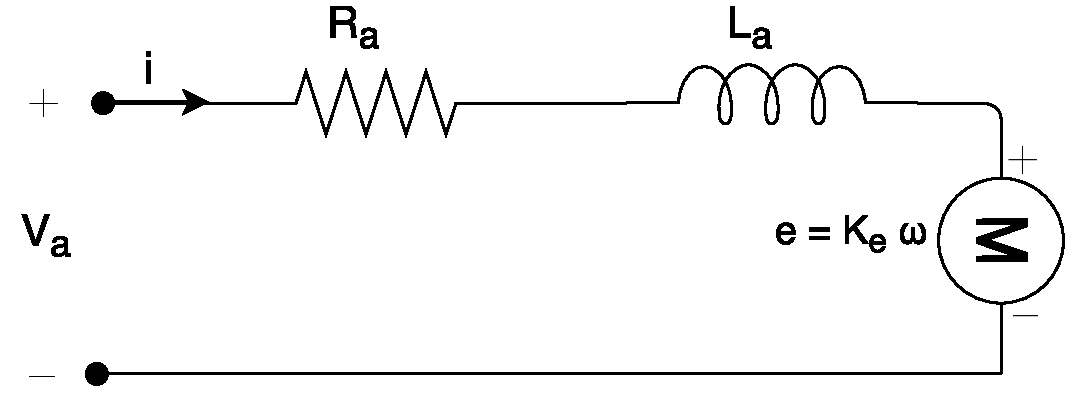
\includegraphics[width=1\linewidth]{figures/BLDC_el.pdf}
			%\caption{ Electrical and mechanical part of the motor }
		%	\label{fig:electromech}
		\end{figure}
	\end{minipage}\hfill
	\begin{minipage}[b]{0.49\linewidth}
		\centering
		\begin{figure}[H]
			\centering
			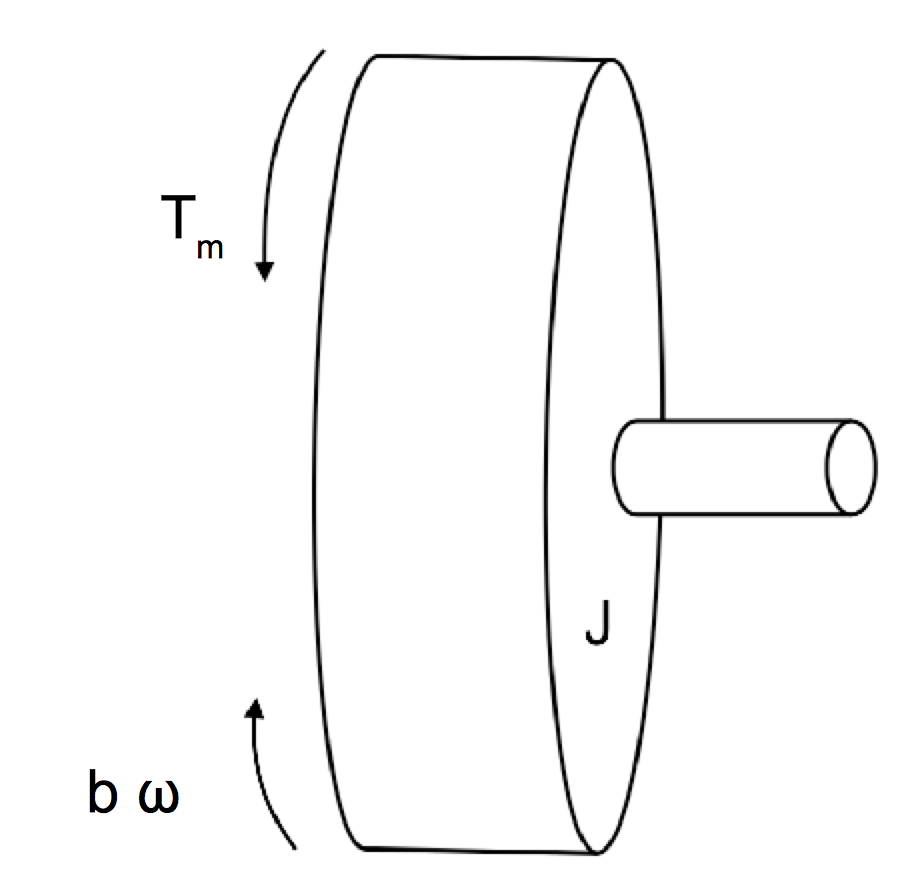
\includegraphics[width=0.55\linewidth]{figures/flywheel_1}
			%\caption{Mechanical part of the motor}
			%\label{fig:distancecontrol4}
		\end{figure}
	\end{minipage}
	\caption{ Electrical and mechanical part of the motor }
	\label{fig:electromech}
\end{figure}

%
The mechanical part of the motor can be modelled as 
%
\begin{flalign}
 k_{t}i  =J\dfrac{d\omega}{dt} + b\omega
	\label{mechpart66}
\end{flalign}
%
%\nomenclature[S]{\textbf{$k_{t}$}}{Motor torque coefficient}
%\nomenclature[S]{\textbf{$b$}}{Viscous friction coefficient}
where $J$ is the rotor moment of inertia, $k_{t}$ [Nm/A] is the motor torque coefficient and $b$ [Nm s/rad] is the viscous friction coefficient. %Assuming the current will not increase rapidly in order not to harm the equipment, and moreover the electrical time constant $\tau_{e}=\dfrac{L}{R}$ is much smaller than the mechanical time constant $\tau_{m}=\dfrac{J}{b}$, the effect of the inductance can be neglected and the
 Equation \ref{mechpart66} can be solved for $i$ and  replaced in \ref{Kirchhoff244}\cite{permanent_magnet}     
%
\begin{flalign}
	i  =\dfrac{J}{k_{t}}\dfrac{d\omega}{dt} + \dfrac{b}{k_{t}}\omega
	\label{mechpart2}
\end{flalign}
%
\begin{flalign}
 V_{a} = \dfrac{LJ}{k_{t}}\dfrac{d^{2}\omega}{dt^{2}}+\dfrac{RJ+Lb}{k_{t}}\dfrac{d\omega}{dt} +\dfrac{Rbk_{e}}{k_{t}}\omega 
	\label{mechpart333}
\end{flalign}
%
by Laplace transformed \ref{mechpart333}, the second order transfer function from $V_{a}$ to $ \omega $ can be written as 
%
\begin{flalign}
	\dfrac{\omega(s)}{V_{a}(s)}= \dfrac{k_{t}}{LJs^{2}+(RJ+Lb)s+(Rb+k_{e}k_{t})}
	\label{tf}
\end{flalign}
%= \dfrac{k_{t}}{LJs^{2}+(RJ+Lb)s+Rb+k_{e}k_{t}}
%\label{tf}
following \cite{permanent_magnet} the electrical time constant $\tau_{e}$ and mechanical time constant $\tau_{m}$ can be written respectively $\tau_{e} = \frac{LJ}{RJ+Lb}$ and $\tau_{m} = \frac{RJ+LB}{RB+k_{e}k_{t}}$, the values for the two time constants are found to be $\tau_{e} = 1.2709\cdot10^{-10}$[s] and $\tau_{m} = 8.4102\cdot10^{-4}$[s] thus since the $\tau_{e}$ is very small compared to $\tau_{m}$, the effect of inductance can be neglected thus the transfer function from $V_{a}$ to $ \omega $ is reduced to a first order transfer function as 
%
\begin{flalign}
\dfrac{\omega(s)}{V_{a}(s)}= \dfrac{k_{t}}{R(Js+b)+k_{e}k_{t}}
\label{tf2}
\end{flalign}
%
the block diagram of the system can be seen in figure \ref{fig:blockdi} along with PI velocity controller which will be discussed in the next section.
%
%\nomenclature[S]{\textbf{$\tau_{e}$}}{Electrical time constant}
%\nomenclature[S]{\textbf{$\tau_{m}$}}{Mechanical time constant}
\begin{figure}[H]
	\centering
	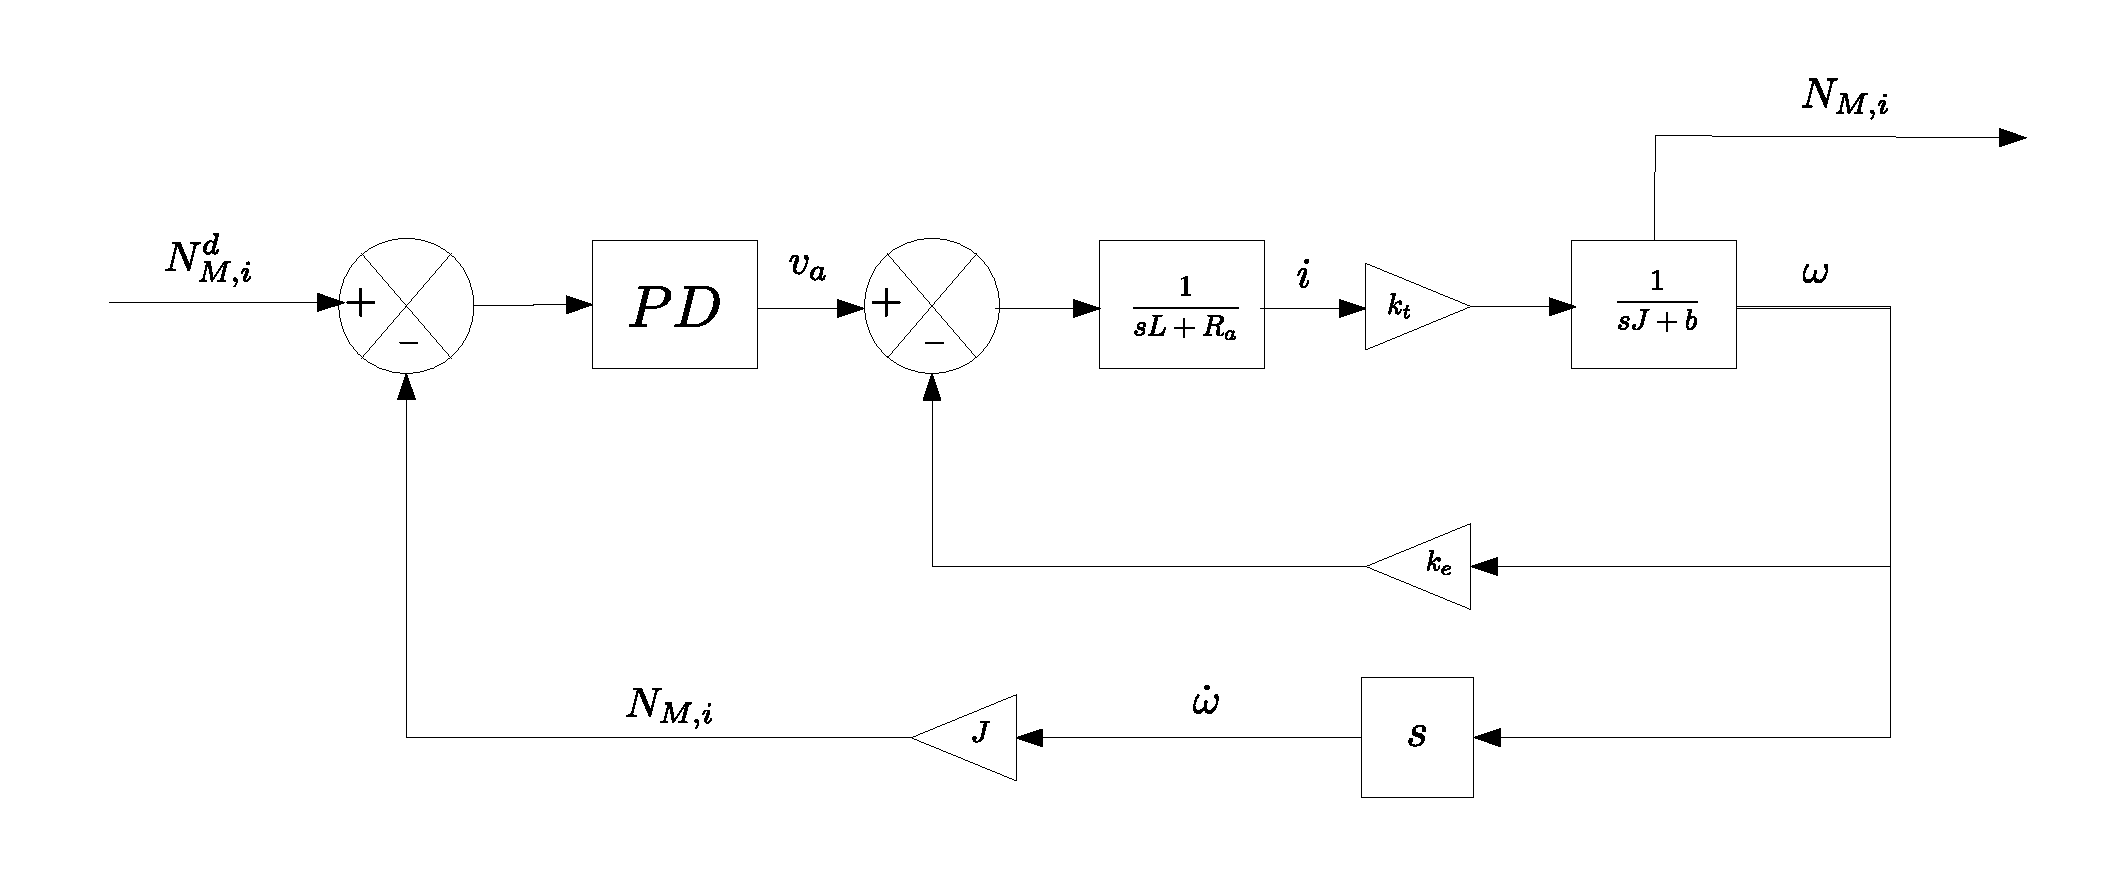
\includegraphics[width=1\linewidth]{figures/omegaControl}
	\caption{Angular velocity controlled DC motor}
	\label{fig:blockdi}
\end{figure}
%

% 
\chapter{Motor control}

\subsection*{ Angular velocity control}

In previous work, two controllers a linear and a non-linear(SMC), have been designed requiring a torque that has to be produced from the motors-wheel system. This torque demand is used to give the desired angular velocity reference for the wheels and thus the torque that will be fed back to the satellite as seen in the \cite{block diagram}. The output torque from the linear and non-linear controllers has three elements which has to be transformed in the tetrahedron configuration using the matrix \eqref{transmatrix}.  A \textit{PID} controller has been designed to control the angular velocity of the motor as seen in the \figref{fig:blockdi222}:
\begin{figure}[H]
	\centering
	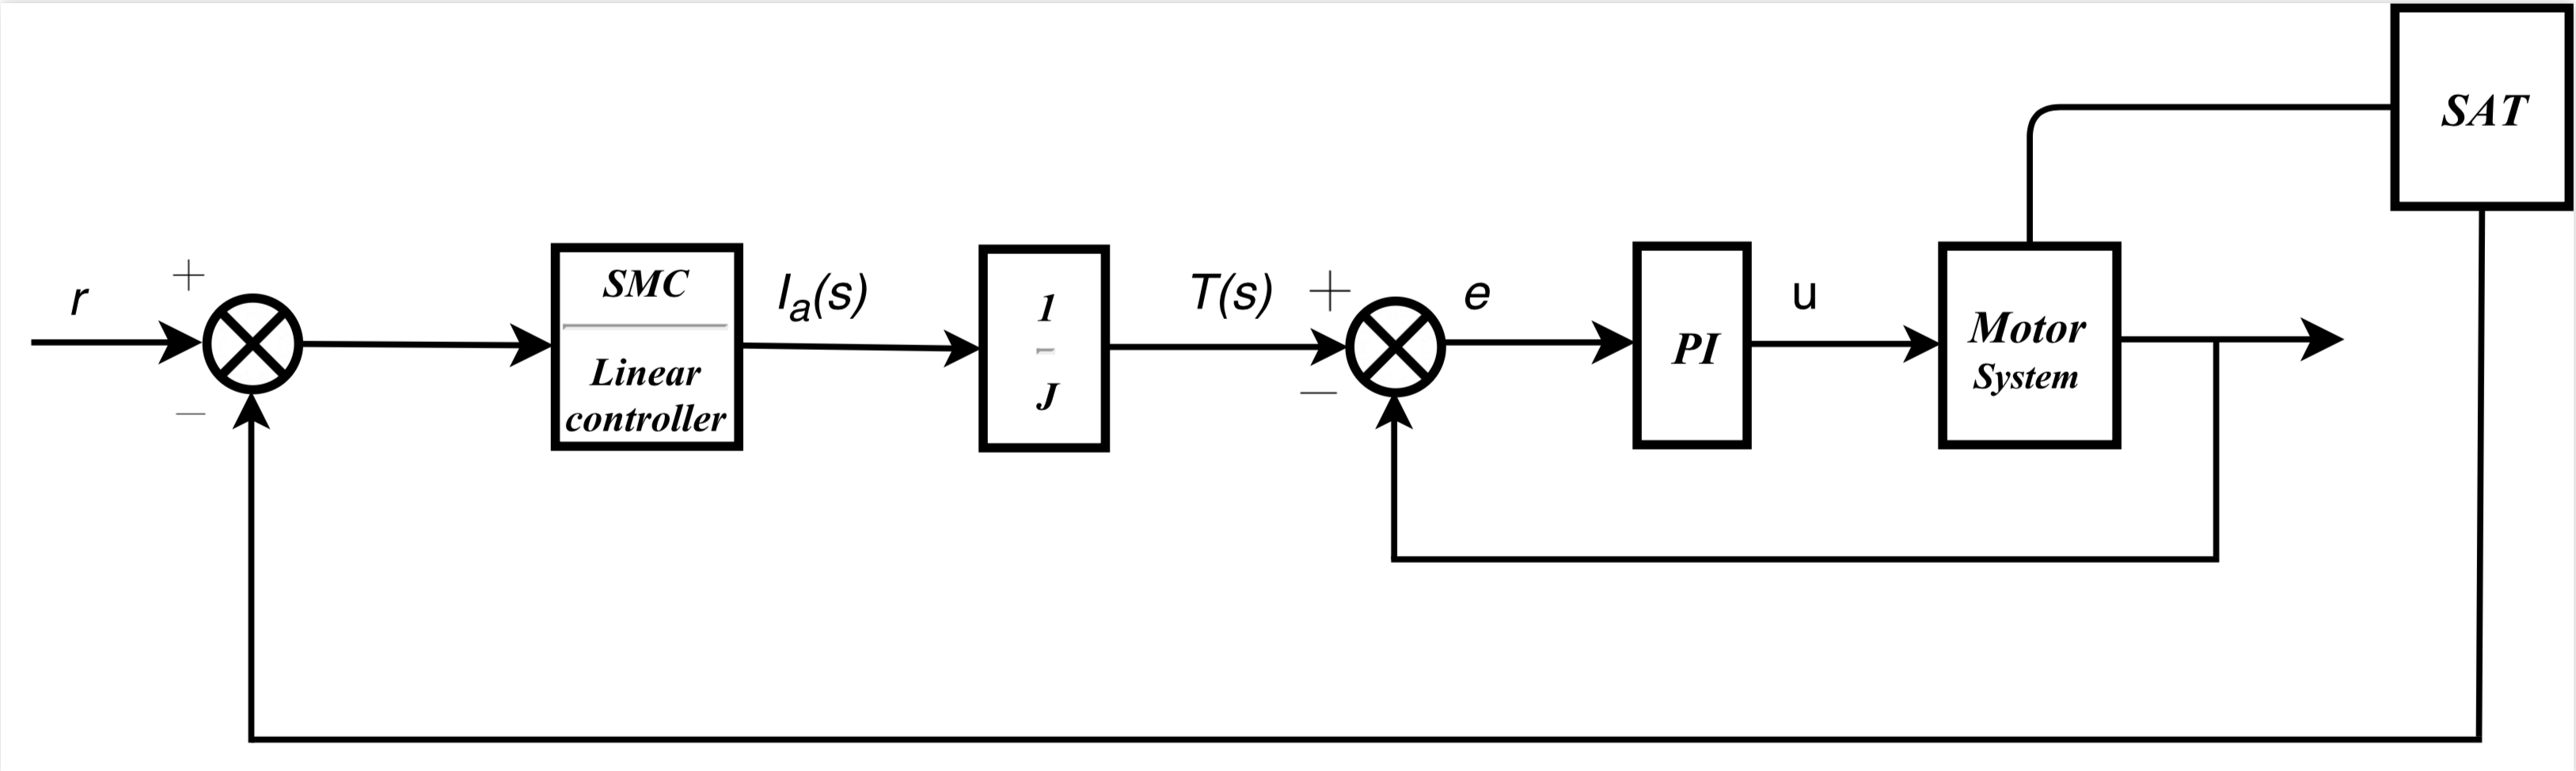
\includegraphics[width=1.0\linewidth]{figures/block_diagram_2}
	\caption{Block diagram of the motor control with PID controller}
	\label{fig:blockdi222}
\end{figure}  
%
The PI controller gains are chosen based on the open loop system response using the Ziegler-Nichols method \cite{PID_tuning} and by trial and error in order to achieve faster closed loop response and asymptotically stable system. The gains are chosen to be:   
%
\begin{flalign*}
	k_{p} = 3.4 \\ k_{i} = 0.9
\end{flalign*}

\todo{make figure bigger}
The root locus of one motor with PI controller is seen in the \figref{fig:rlocus33}
%
\begin{figure}[H]
	\centering
	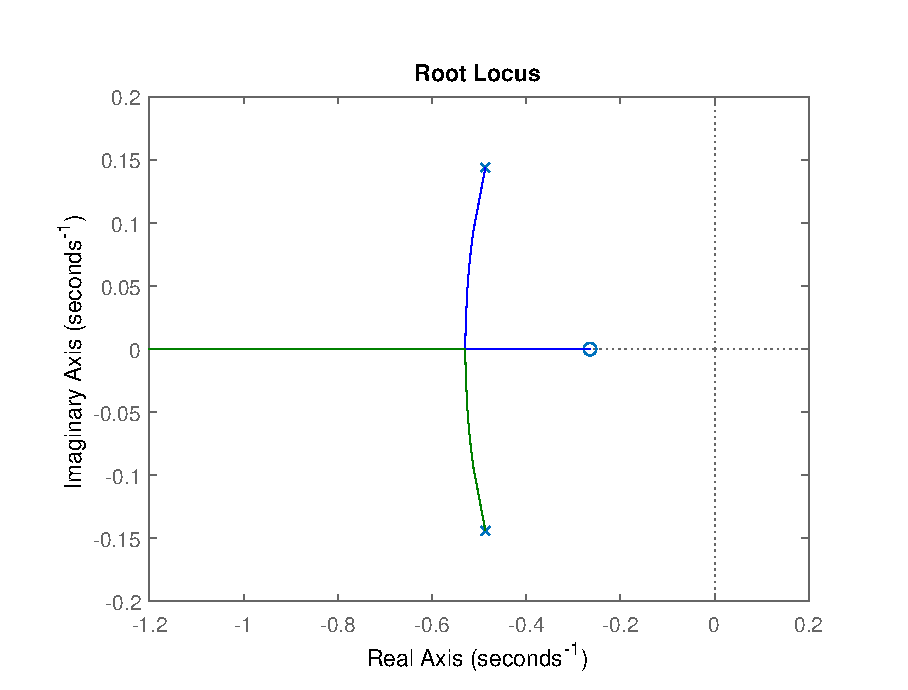
\includegraphics[width=0.7\linewidth]{figures/pid_rootlocus}
	\caption{Root locus of one motor with PI controller}
	\label{fig:rlocus33}
\end{figure}
%
The closed loop system gives complex eigenvalues and fast response and is stable for a wide range of the adjustable parameters. 
%

%

\subsection{Torque Control}

The main attitude controller sends a torque demand to the actuators, which is then distributed between the actuators. Each of the reaction wheels get their own individual torque demand signals. Two methods have been implemented for tracking this torque demand. One is by transforming the torque to angular velocity demand, which the motor has to track, the other is directly controlling for actuator error.

\begin{figure}[h!]
	\centering 
	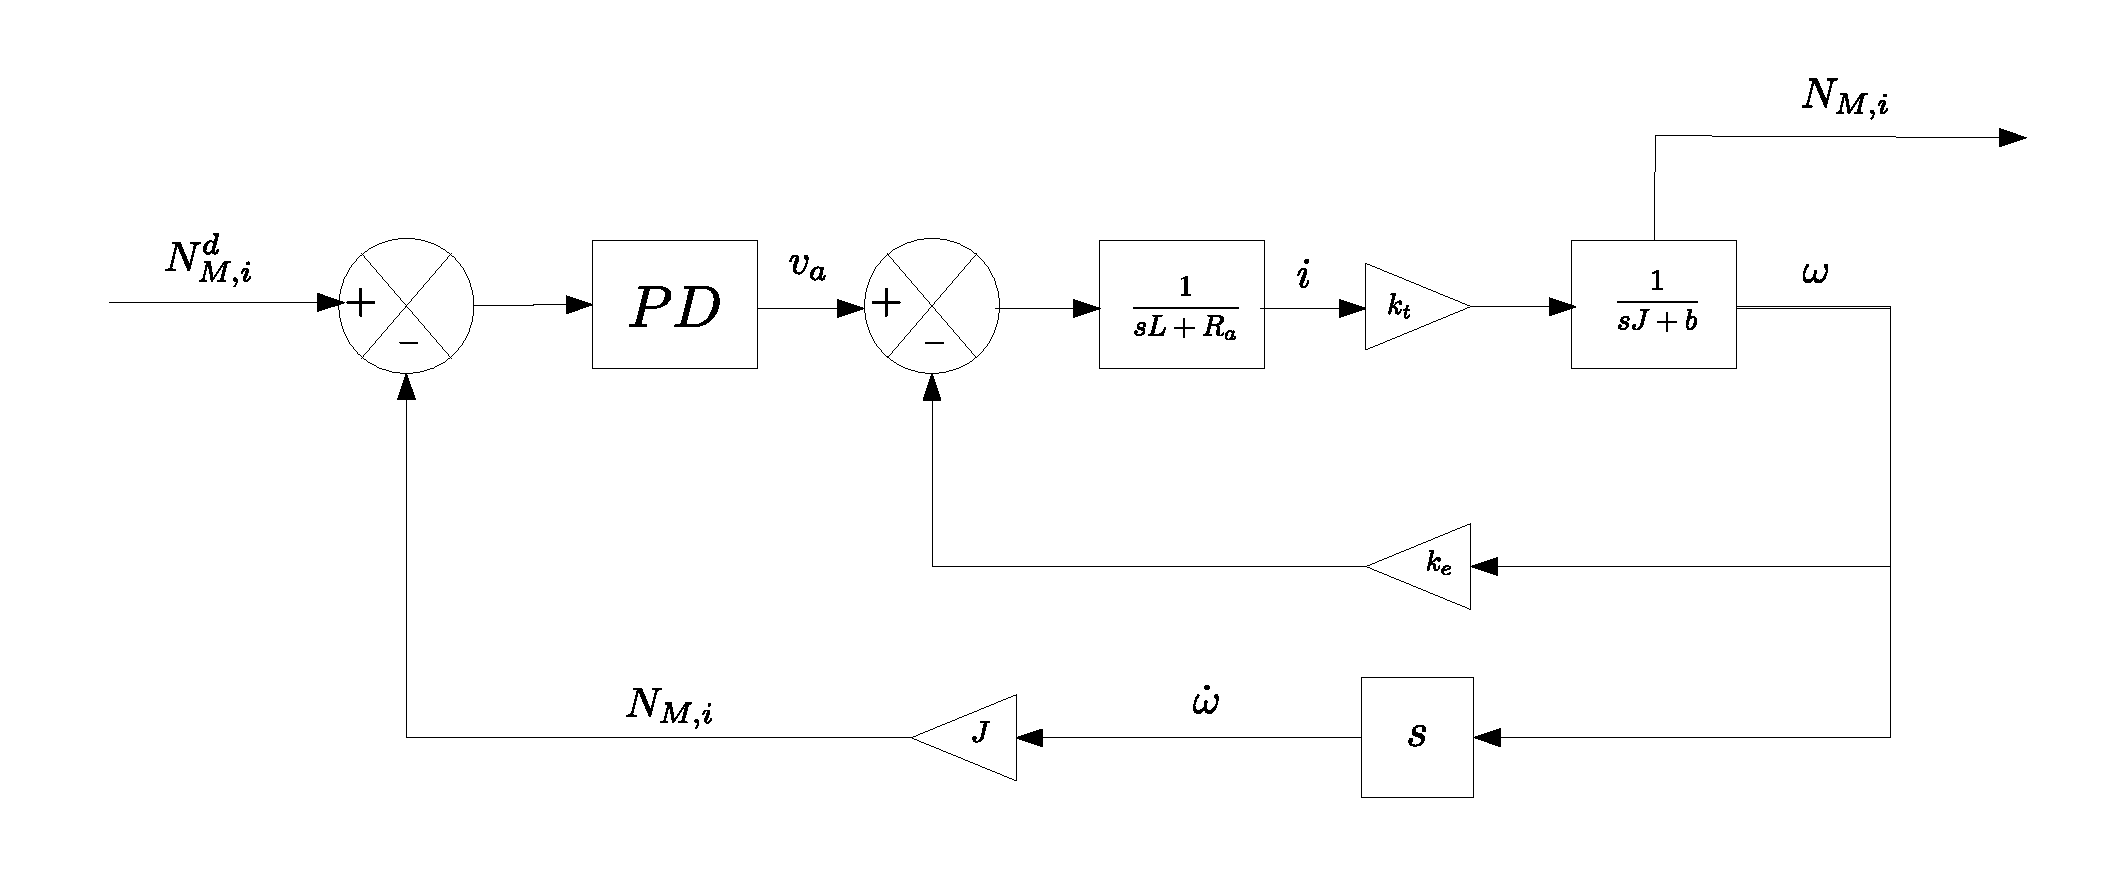
\includegraphics[width=170mm]{figures/torqueControl.pdf}	
	\caption{Torque control scheme.}
	\label{label{fig:frames}}
\end{figure}

As shown on Figure XY , the torque controller controls the torque error signal using a PD controller. Since the torque has a $ 10^{-5} Nm$ magnitude, while the voltage has $ 10^1 V$, numerically the PD gains are quite large. The control signal is the input voltage for the DC motor. The subsystem is second order, including an integrator for current and one for angular velocity.

\section*{Magnetorquer model}
\nomenclature[Sncoil]{$n_{coil}$}{The number of windings of the coil}
\nomenclature[SIcoil]{$I_{coil}$}{The electric current flowing through the coil}
\nomenclature[SAcoil]{$\vec A_{coil}$}{The vector perpendicular to the cross-sectional area of the magnetorquer}
\nomenclature[Sm]{$\vec m_{mt}$}{The magnetic dipole moment}

Since the primary actuators for the satellite are chosen to be reaction wheels, four magnetorquer will be used for desaturation of the reaction wheels.  

Having a solenoid onboard of the satellite, referred as a magnetorquer through which the current could be controlled and hence the dipole moment.

The interaction of the dipole with the magnetic field of the Earth will result in a torque that will be perpendicular to the magnetic field vector according to the following equation \cite{SADC}:
\begin{flalign}
   \vec N_{mt} = \vec m_{mt} \times \vec B
	\label{eq:NT}
\end{flalign} 
where $\vec N$ is the torque produce by the magnetorquer and will be the torque that will influence the satellite dynamics, $\vec B$ is the vector of the magnetic field of the Earth and $\vec m_{mt} $ is the magnetic dipole moment generated by the magnetorquer.

The magnetic moment $\vec m_{mt}$ is given by \cite{MagMom}:
\begin{flalign}
	\vec m_{mt} = n_{coil} \ I_{coil} \ \vec A_{coil}
	\label{eq:mm}
\end{flalign} 
where $n_{coil}$ is the windings of the coil, $I_{coil}$ is the electric current on the coil and $\vec A_{coil}$ is the vector perpendicular to the cross-sectional area of the magnetorquer.

Using \ref{eq:NT} and \ref{eq:mm} and taking the magnitude, the applied torque on the satellite is \cite{SJ}:
\begin{flalign}
	\vec N_{mt} = n_{coil} \ \rvert I_{coil}\rvert \ \rvert \vec A_{coil}\rvert \ |\vec B| \sin (\theta)
	\label{eq:ft}
\end{flalign} 
where $\sin (\theta)$ is the angle between the plane $A_{coil}$ and the magnetic field vector $\vec B$.

Furthermore, the resistance of the magnetorqer which is a function of the temperature of the coil given as an input, can be computed as
\begin{flalign}
R_{mt} = \dfrac{nC  \rho_{mt} }{A_{wire}} = \dfrac{nC \rho_0(1+\alpha_0(T_{mt} - T_0))}{A_{wire}}
\label{eq:rt}
\end{flalign} 
where \\
$R_{mt}$ is the resistance of the magnetorquer \\
$n$ is the number of windings \\ 
$C$ is the wire circumference  \\
$A_{wire}$ is the wire cross-sectional area  \\
$\rho_0$ is the resistivity of copper  \\
$\alpha_0$ is the coefficient of resistivity temperature   \\
$T_{mt}$ is the temperature given as an input   \\
$T_0$ is the resistivity base temperature  

Using the computed resistance the current is found by dividing the voltage by the resistance of the magnetorquer. Next, in order to find the magnetic moment $m$, the current is multiplied by the number of windings and the area of the wire. For finding the torque that acts on the satellite, the magnetic moment is multiplied by the coil normal and a cross-product is used between this multiplication and the magnetic field of the Earth.

In order to find what voltage to output for having a certain amount of torque, a gain between voltage and magnetic moment is found. For the coil model, the control signal is the voltage. Therefore, translating the magnetic moment demand to voltage is found as follows:
\begin{flalign}
\frac{\vec m_{mt}}{v} = \frac{n_{coil} \vec A_{coil} \vec I_{coil}}{R_{mt}} \mathcal {K}
	\label{eq:gain}
\end{flalign} 
\begin{flalign}
 \mathcal{K} = \frac{\vec m_{mt} R_{mt} }{ n_{coil}  \vec A_{coil} \vec I_{coil} v}
	\label{eq:gainn}
\end{flalign} 
where \\
$v$ is the voltage \\
$\mathcal {K}$ is the gain

The voltage can be found using the following transfer function:
\begin{flalign}
	\frac{I_{coil}}{v} = \frac{1}{R_{mt}}
	\label{eq:voltage}
\end{flalign} 

where the voltage is found to be $1.25 V$

Given a current $I$ going through a coil, the interest is to find the magnetic field $B$ at a certain point located distance $r$ from the coil. Finding an estimate of the magnetic field at any point will give the possibility to change the location of the magnetometers around. For computing the magnetic field in the center of a rectangular coil, the law of Biot-Savart is used \cite{SJ}:
\begin{flalign}
	d\vec B = \frac{\mu_0 I}{4 \pi}  \frac{d \vec s \times \hat{\vec r}}{r^2}
	\label{eq:BS}
\end{flalign} 
where \\
$\vec B$ is the magnetic field \\
$\mu_0$ is a constant called permeability of free space and is equal with $4\pi \times 10^{-7}  \ Tm/A$ \\
$I$ is the current \\
$d \vec s $ is a length element in the direction of current \\
$\hat{\vec r}$ is the direction from $d \vec s$ to a particular position \\
$r$ is the distance from $d \vec s$ to a particular position

The magnetic field $B$ at any point is directly proportional to the current $I$ that is crossing the coil. The magnetic field generated by the current from equation \ref{eq:BS} is just a small length element $d \vec s$ of the coil. For finding the total magnetic field, all small elements need to be summed up and for this the magnetic field $B$ have to be evaluated by integrating equation \ref{eq:BS}.

The design of the magnetorquer is described in appendix \ref{chap:F}.

\chapter{Control Schemes}
\textit{The satellite control schemes are introduced starting from the top of the hierarchy. The chosen reaction wheel desaturation control scheme determines the overall control structure, while allowing modification of other control blocks, making the system modular. Three different main attitude controllers are discussed}.

%\sout{In this chapter the purpose is to describe the design of the controllers for the satellite. First, a desaturation controller is designed for distributing the torque between the actuators. A second controller is the hybrid attitude one, which is capable of taking care of the tumble of the satellite. Next, based on previous work, two types of attitude controllers are designed. For making a comparison between a linear controller and non-linear one, a state feedback controller and a sliding mode controller are presented.}

When developing complex systems, using a modular design, setting up a hierarchy between elements, and using abstractions can be very helpful in keeping the complexity at a manageable level. They can also prove to be useful during debugging or finding faults in the system. The proposed control scheme utilizes these tools. Figure  \ref{fig:mainLoop} introduces the high-level control scheme used in the thesis. The scheme is inspired by the control scheme proposed by Trégouët et al. in their paper concerning a new desaturation control scheme \cite{DesatTregouet}. 

%The proposed high-level control scheme presented in figure \ref{fig:mainLoop} has a hierarchical, modular structure.
 The main attitude controller outputs a torque reference for the actuators, which is then distributed by lower level controllers. This means that the attitude controller can be swapped without having to modify the lower level controllers. The desaturation controller distributes the torque between the reaction wheels and magnetorquers. The reaction wheel subsystem executes local fault detection and fault isolation. It receives a three dimensional torque demand and distributes it between the individual reaction wheel motors. The reaction wheel subsystem checks fault residual signals and adjusts torque distribution between reaction wheels accordingly. These will be elaborated in subsequent sections.
 
\begin{figure}[h!]
	\centering 
	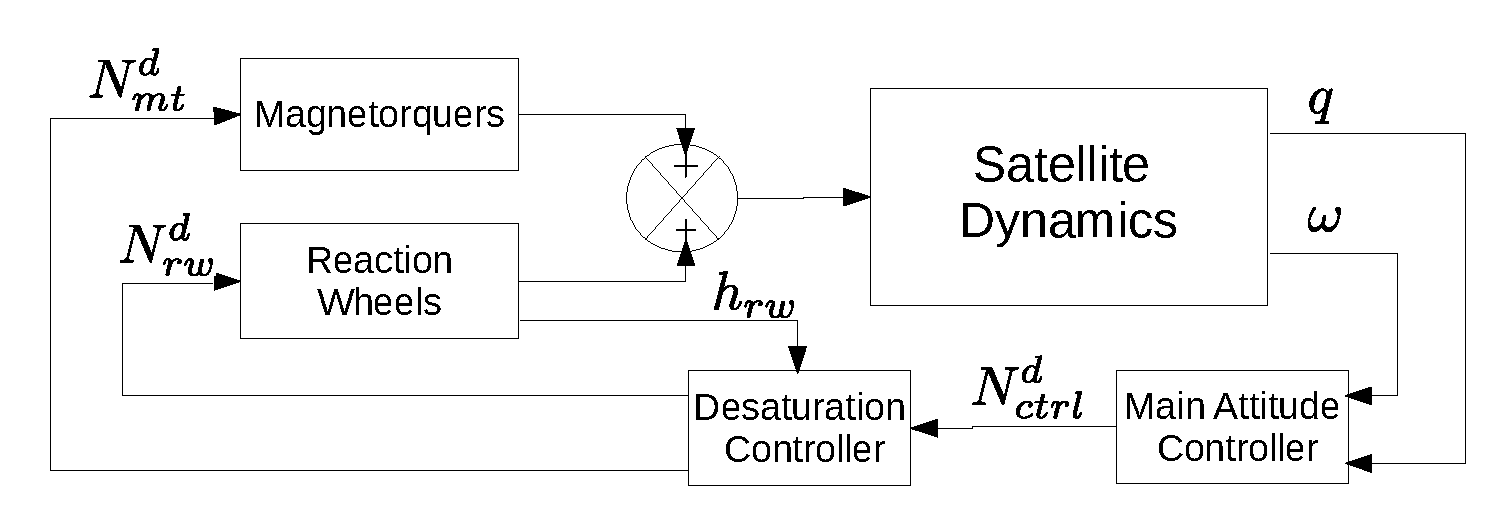
\includegraphics[width=160mm]{figures/mainLoop.pdf}	
	\caption{Main Control Loop.}
	\label{fig:mainLoop}
\end{figure}

		\begin{equation}
		\underline{I}_{s}\vec{\dot{\omega}} + \underline{\omega}^\times\underline{I}_{s}\vec{\omega} = -\vec{\dot{h}}_{rw} -  \underline{\omega}^\times \vec{{h}}_{rw} + \vec{N_{mt}}  + \vec{N_{dist}} =  -  \underline{\omega}^\times \vec{{h}}_{rw} + \vec{N_{rw}} + \vec{N_{mt}}  + \vec{N_{dist}} 
		\end{equation}
		
\section{Desaturation}

The reaction wheel DC motors and bearings have a limited angular velocity range they can operate in. When the velocity reaches the limit, the motor can no longer accelerate the wheel further in one direction, thus reducing controllability. To avoid this, the wheel velocity should be kept near zero. Usually the speed is above zero to avoid static friction in the bearings. Decreasing the reaction wheel speed by transferring its angular momentum is called desaturation.

Reaction wheels are used to control the attitude of the satellite by transferring its angular momentum. Transferring the angular momentum back to the satellite body would be counterproductive, it should be discarded in a different way. Magnetorquers are ideal for desaturation since they can interact with the earth's magnetic field and are able to transfer angular momentum of the satellite body to earth. Since the earth's magnetic field is quite weak, the torque produced by magnetorquers are small compared to the torque of the reaction wheels. Reaction wheels can be used for fast attitude control while magnetorquers are good for gradually desaturating the reaction wheels. The angular momentum transfer happens through the satellite's body, but with the right control scheme the desaturation can be  completely decoupled from attitude control.

Trégouët et al. \cite{DesatTregouet} developed a cascaded control method for reaction wheel desaturation. The method is a revised version of the so-called cross-product control law. It changes the magnetorquers' magnetic field based on the difference between the angular momentum of the reaction wheels and their reference angular momentum.

\begin{equation}
\vec{\tau_m} = -\frac{\underline{\tilde{b}}^\times(t)}{|\vec{\tilde{b}}(t) |^2} k_p\left(\vec{h_{rw}} - \vec{h_{ref}} \right)
\end{equation}

where  \todo{add the notations to nomenclature}

Momentum dumping and attitude control can potentially be opposing goals, since attitude control changes the reaction wheel velocity to produce the required torque, while the desaturator tries to keep the angular velocity close to the reference. The quasi-cascaded structure of the desaturation control law includes the magnetorquer as the upper subsystem which outputs the rate of change of the total angular momentum of the system \ref{fig:CascadeDesat}. The lower subsystem includes the attitude dynamics and the reaction wheel controller. The problem is that there's a feedback involved from the lower subsystem to the upper one, making $\dot{h}_t$ dependent on the attitude parameters. This means that desaturating the wheels can affect the attitude control loop. Since attitude control is more crucial than desaturation, the reverse would be desirable.  By reversing the ordering of the cascade, the interference can be eliminated. It is done by applying input allocation, i.e. "suitably assigning the low level actuators' input, based on a higher level control effort requested by the control system" \cite{JOHANSEN20131087}. From the point of view of the desaturation controller, the control goal is to keep the reaction wheels' angular velocity as close to the reference velocity as possible. Since the desaturation control is decoupled from attitude control, it can achieve its desaturation control goal regardless of the attitude control law.




\begin{figure}[h]
	\centering
	\begin{tabular}{@{}c@{\hspace{.5cm}}c@{}}
		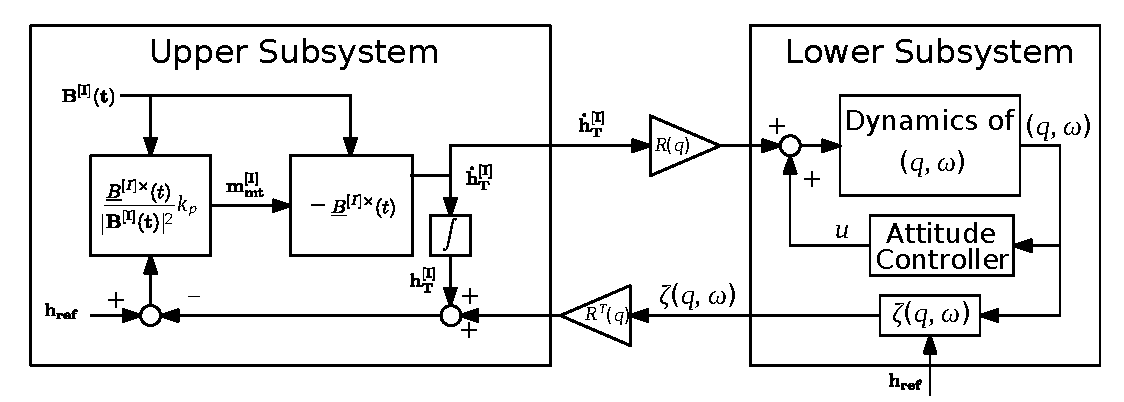
\includegraphics[page=1,width=1\textwidth]{quasiCascadeDesat.pdf}
	\end{tabular}
	\caption{Quasi cascaded desaturation control scheme \cite[Fig. 2.]{DesatTregouet}}
	\label{fig:quasiCascadeDesat}
\end{figure}

According to equation \todo{ref eq in modelling}

\begin{equation}
\underline{I}_{s}\vec{\dot{\omega}} + \underline{\omega}^\times\underline{I}_{s}\vec{\omega} = -\vec{\dot{h}}_{rw} -  \underline{\omega}^\times \vec{{h}}_{rw} + \vec{N_{mt}}  + \vec{N_{dist}} = \vec{u} 
\end{equation}

\begin{equation}
\vec{\tau_m}^{[I]} = -\frac{\underline{\tilde{b}}^\times(t)}{|\vec{\tilde{b}}(t) |^2} k_p\left(\vec{h_{rw}}^{[I]} - \underline{R}^T(\vec{q})\vec{h_{ref}} \right)
\end{equation}

\todo{make it a system of equations}

%\begin{equation}
%\dot{x}_c = 0, (\vec{q},\vec{\omega},x_c) \in C\
%\end{equation}
%
%\begin{equation}
%x_c^+ = -x_c, (\vec{q},\vec{\omega},x_c) \in D\
%\end{equation}
%
%\begin{equation}
%\vec{u} = -c x_c \epsilon -K_\omega \vec{\omega}
%\end{equation}
%
%\begin{equation}
%C:= \left\lbrace (\vec{q},\vec{\omega},x_c) \in \mathbb{S}^3 \times \mathbb{R}^3 \times \left\lbrace -1,1 \right\rbrace : x_c\eta \geq -\delta \right\rbrace 
%\end{equation}
%
%\begin{equation}
%D:= \left\lbrace (\vec{q},\vec{\omega},x_c) \in \mathbb{S}^3 \times \mathbb{R}^3 \times \left\lbrace -1,1 \right\rbrace : x_c\eta \leq -\delta \right\rbrace 
%\end{equation}

as shown in \ref{eq:finaleq}
\begin{flalign}
\vec{ ^s_i\dot q(t)}  = \dfrac{1}{2} \underline \Omega \  \vec{^s_i q(t)}
\end{flalign} 

\[
\begin{array}{l}

\dot{x}_c = 0, (\vec{q},\vec{\omega},x_c) \in C\ \\ 
x_c^+ = -x_c, (\vec{q},\vec{\omega},x_c) \in D\ \\ 
\vec{u} = -c x_c \epsilon -K_\omega \vec{\omega} \\
C:= \left\lbrace (\vec{q},\vec{\omega},x_c) \in \mathbb{S}^3 \times \mathbb{R}^3 \times \left\lbrace -1,1 \right\rbrace : x_c\eta \geq -\delta \right\rbrace  \\

D:= \left\lbrace (\vec{q},\vec{\omega},x_c) \in \mathbb{S}^3 \times \mathbb{R}^3 \times \left\lbrace -1,1 \right\rbrace : x_c\eta \leq -\delta \right\rbrace 
\end{array}
\]

\todo{this attitude controller should be down as one of the possible attitude controllers - "Satellite angular momentum removal utilizing the earth’s magnetic field" article}

\begin{figure}[h]
	\centering
	\begin{tabular}{@{}c@{\hspace{.5cm}}c@{}}
		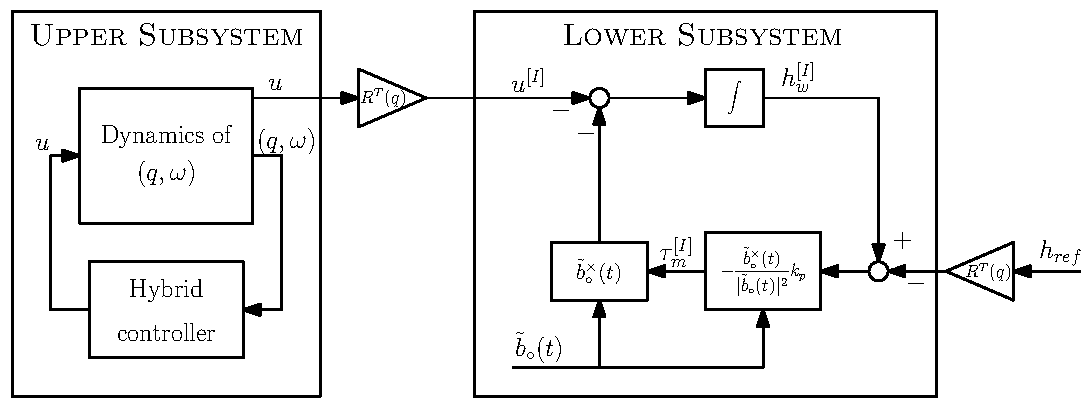
\includegraphics[page=1,width=1\textwidth]{cascadeDesat.pdf}
	\end{tabular}
	\caption{Cascaded desaturation control scheme  \cite[Fig. 4.]{DesatTregouet}}
	\label{fig:CascadeDesat}
\end{figure}

The derived equations that can be implemented in simulation:

\begin{equation}
\vec{\dot{\omega}} = \underline{I}_{s}^{-1}\left( \vec{u} -  \underline{\omega}^\times\underline{I}_{s}\vec{\omega}  \right) 
\end{equation}

\begin{equation}
\vec{\dot{h}}_{rw} =  -  \underline{\omega}^\times \vec{{h}}_{rw} + \vec{N_{mt}}  + \vec{N_{dist}} - \vec{u} 
\end{equation}

\todo{body-fixed frame
	Static input allocation
	global asymptotic stability}

\cite{DesatYang}
\section{Attitude Reference}

The main attitude controllers require an attitude reference quaternion and a reference angular velocity to track. In the simulation environment, the attitude reference quaternion is given in orbit frame, the angular velocity reference in ECI frame. As discussed above, two attitude control goals are distinguished: nadir pointing and Earth station tracking. For nadir pointing, the attitude reference quaternion is simply assigned as $[0 \ 0 \ 0 \ 1]^T$ and the angular velocity reference is identical to the orbit angular velocity. Creating the references for Earth station tracking are not as trivial.

For Earth station tracking, the reference quaternion can be calculated using the positions of the satellite, the station, and the center of Earth. The unit rotation axis of the attitude quaternion is $\vec{e} = \frac{^{sat}\vec{R}_{o} \times ^{sat}\vec{R}_{st}}{||^{sat}\vec{R}_{o} \times ^{sat}\vec{R}_{st}||}$, where ${^{sat}\vec{R}_{o}}$ is the distance from center of Earth to the satellite and $^{sat}\vec{R}_{st}$ is the distance from station to the satellite. 

The angle between the nadir pointing and the station pointing vectors can be calculated using the law of cosines. The attitude quaternion in orbit frame is calculated using the quaternion rotation formula $ \vec q = e^{\frac{\Phi}{2} (e_1 \textbf{i}+ e_2 \textbf{j} + e_3 \textbf{k} + e_4)} = \cos \frac{\Phi}{2} + (e_1 \textbf{i}+ e_2 \textbf{j} + e_3 \textbf{k}) \sin \frac{\Phi}{2}$, as described in appendix \ref{chap:A}. The corresponding angular velocity reference can be calculated using the equation described in appendix \ref{eq:finaleq}.



%For the satellite to be able to track a given static position on Earth within 1°, a quaternion is computed. Therefore, this quaternion represents the vector that points from the orbit position to the station.
%
%The tracking quaternion is calculated by giving a quaternion attitude demand in orbit frame and by using this it is possible to calculate the angular velocity demand. The position vector of the station and the position of the satellite are known, then this two are subtracted and results the direction between them which is transformed into a quaternion.
%
%In the simulation the Earth station is stationary which means that it does not move in the inertial frame.
%
%The way it can be verify that the error is around 1°, is by looking at the attitude error quaternion.  The scalar part which represent $\cos (\frac{\alpha}{2}) $ and then calculate $\alpha$ based on that.  That $\alpha$ it should not be bigger then 1°.

\begin{figure}[H]
	\centering
	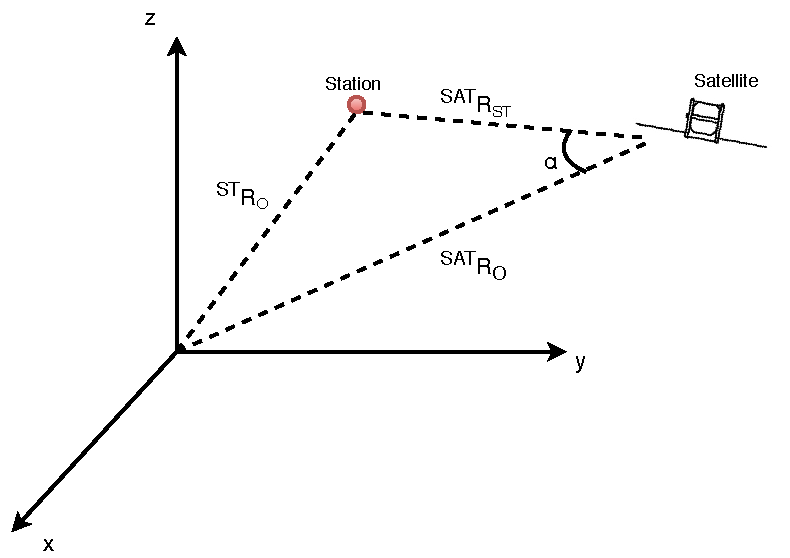
\includegraphics[width=0.7\linewidth]{figures/ST}
	\caption{Tracking a target on Earth }
	\label{fig:TS}
\end{figure}

\section{Main Attitude Controller}
\label{sec:mainCont}

\textit{Previously the main attitude controller was treated as a black box. The current and subsequent sections discuss several satellite attitude controllers.}

\subsection{Hybrid Attitude Controller}

Dynamic discontinuous hybrid controller, global asymptotic stability, local exponential stability, state feedback for $\omega$ and $q$. Capable of detumbling. \cite{globalAttController}

There are different ways to describe the rotation of a 3D object. One of them is by using Euler sequences consisting of 3 rotational values. Euler rotation sequences can use combinations of roll, pitch and yaw. There's an inherent problem with Euler rotation, that makes controlling Euler rotation based models an issue, i.e. they are susceptible to singularities. Certain orientations might have an infinite amount of corresponding Euler angles. This can arise when the rotations are made in such a way that some rotation axes align with each other. This issue is commonly known as the gimbal lock. The result of a gimbal lock is that given an attitude, the  cannot be unambiguously deducted, unless extra constraints are introduced.

Quaternion based rotation representation are more appropriate for control. Quaternions are not susceptible to singularities. The only problem with quaternion representation is the so-called double coverage, i.e. rotation by $-\vec{q}$ represents the same rotation as rotation by $-\vec{q}$. This becomes obvious from the rotation equation \ref{eq:doubleCover}.

\begin{equation}
\label{eq:doubleCover}
\vec{q} \vec{v} \vec{q}^{-1} = 	(\vec{-q}) \vec{v} (\vec{-q}^{-1})
\end{equation} 

The attitude control goal can be described as tracking the orientation demand $\vec{q}$. According to \cite{globalAttController}, it is impossible to design a globally stabilizing quaternion based state feedback that is robust to measurement noise. The quaternion-based robust hysteretic feedback controller which is capable of globally asymptotically stabilizing a rigid body is described subsequently, according to \cite{globalAttController}. It can be considered as a more robust extension of classical state feedback controller.


The dynamics of a rigid body is described in equation \ref{eq:dynSimple1}. For clarity of the control method, disturbance torques are emitted from the equation. Since the control system compensates for the gyroscopic term, it is omitted as well from the discussion .

\begin{equation}
\label{eq:dynSimple1}
\underline{I}_s \vec{\dot{\omega}} = \underline{\omega}^\times \underline{I}_s \vec{\omega} + \vec{N_{ctrl}}
\end{equation}

The control goal can be clearly described with rotation matrices. Rotation matrices use 9 variables to describe a rotation, but they have the advantage of being non-ambiguous. The rotation error can be described using equation \ref{eq:rotationError}. 

\begin{equation}
\label{eq:rotationError}
\underline{R}(\vec{q^e}) = \underline{R}(\vec{q^d})^T \underline{R}(\vec{q})
\end{equation}

The goal is to align $\underline{R}(\vec{q})$ with $\underline{R}(\vec{q^d})$ orientation demand. If that demand is satisfied, $\underline{{R}}(\vec{q^e})$ orientation error becomes $\underline{I}$ identity matrix. In quaternion representation, this goal corresponds to having having a unit quaternion with the scalar element being $\pm 1$, according to equation \ref{eq:stabilityQuat}. 

\begin{equation}
\label{eq:stabilityQuat}
\underline{R}(\vec{q^e}) = \underline{R}(\vec{q^e}) = \underline{1} \xrightarrow{equivalent} \vec{q^e}  = \pm	\begin{bmatrix}
0 \\
0 \\
0 \\
1
\end{bmatrix} 	
\end{equation}

Because of the double coverage property of quaternions, stabilizing an attitude, stabilization has to be done on a two equilibrium points corresponding to $\vec{q^e}$ in equation \ref{eq:stabilityQuat}. If a feedback controller is used in the form of $\vec{N_{ctrl}} = f(\vec{q^e})$, $\vec{q^e}$ and $-\vec{q^e}$ might result in different torque demand, even though they both represent the same rotation. The hybrid controller addresses this issue. According to \cite{globalAttController}, robust and global stabilization on this set is impossible to achieve using non-hybrid discontinuous state feedback in the presence of sensor noise. The paper proposes a hybrid, discontinuous, hysteretic, robust, gloablly asymptotically stabilizing attitude control method instead. A system is considered a hybrid system in the subsequent discussion if the state changes can vary between being continuous or discrete.

The state changes are controlled by the following rules. Controller state storing information about which of the double covering quaternions should be tracked is introduced as $x_c \in  \left\lbrace -1,1 \right\rbrace $. $x_c$ decides which of the two double covering quaternions should be tracked. If $x_c = signum(q_4)$ rule is followed, the controller becomes sensitive to measurement noise. To avoid that, a hysteresis introduced, with an adjustable $\delta  \in (0,1)$ hysteresis threshold parameter. The rule for choosing between discrete or continuous control mode is presented in equation \ref{eq:contDiscont}.

\begin{align}
\label{eq:contDiscont}
C:= \left\lbrace (\vec{q},\vec{\omega},x_c) \in \mathbb{S}^3 \times \mathbb{R}^3 \times \left\lbrace -1,1 \right\rbrace : x_c q_4 \geq -\delta \right\rbrace  \\
\nonumber D:= \left\lbrace (\vec{q},\vec{\omega},x_c) \in \mathbb{S}^3 \times \mathbb{R}^3 \times \left\lbrace -1,1 \right\rbrace : x_cq_4 \leq -\delta \right\rbrace 
\end{align}

If $(\vec{q},\vec{\omega},x_c) \in C$, i.e. the controller is running in continuous mode, the governing equations are according to equation \ref{eq:globalCont}. When $(\vec{q},\vec{\omega},x_c) \in D$, $x_c$ controller state swaps sign instantaneously. Because of the $\delta$ thresholding, two swaps don't happen in infinitesimally small time.  

\begin{align}
	\label{eq:globalCont}
\dot{x}_c = 0, & (\vec{q},\vec{\omega},x_c)  \in C \\
\label{eq:globalDiscont}
x_c^+ = -x_c, & (\vec{q},\vec{\omega},x_c) \in D\
\end{align}

Equation \ref{eq:globalControlInput} describes the generated negative feedback control signal. $K_q$ is the adjustable orientation error gain, $K_e$ is an also adjustable parameter for angular velocity gain.

\begin{equation}
\label{eq:globalControlInput}
\vec{u} = -K_q x_c \vec{q^e}_{1:3} -K_\omega \vec{\omega^e}
\end{equation}

%\begin{align}
%	\label{eq:contDiscont}
%	x_c q_4 \geq -\delta \xrightarrow{}  Continuous \\
%	\nonumber x_c q_4 < -\delta \xrightarrow{}  Discontinuous
%\end{align}

\todo{add to nomenclature}
\todo{graphs}


%\[
%\begin{array}{l}
%%\dot{x}_c = 0, (\vec{q},\vec{\omega},x_c) \in C\ \\ 
%x_c^+ = -x_c, (\vec{q},\vec{\omega},x_c) \in D\ \\ 
%%\vec{u} = -c x_c \epsilon -K_\omega \vec{\omega} \\
%%C:= \left\lbrace (\vec{q},\vec{\omega},x_c) \in \mathbb{S}^3 \times \mathbb{R}^3 \times \left\lbrace -1,1 \right\rbrace : x_c\eta \geq -\delta \right\rbrace  \\
%%
%%D:= \left\lbrace (\vec{q},\vec{\omega},x_c) \in \mathbb{S}^3 \times \mathbb{R}^3 \times \left\lbrace -1,1 \right\rbrace : x_c\eta \leq -\delta \right\rbrace 
%\end{array}
%\]

\subsubsection{Detumbling}

After a satellite is ejected from its rocket, it might be rotating quite fast. The first task of the satellite attitude controller is detumbling the satellite, preparing for normal operation. The hybrid attitude controller is capable of doing that. This means that the hybrid attitude controller is a good nominee for being the attitude controller for every operation mode. A simulation was made where the satellite's initial angular velocity is unrealistically high, the goal being to stabilize the satellite to point at the nadir. The controller saturates at $\pm 2 \dot 10^{-3} Nm$, characteristic of the reaction wheels. At the current level of analysis, motor and magnetorquer models are omitted, it is assumed that the actuators satisfy the attitude controller's torque demand. Simulation results with actuator models are presented in subsequent chapters.
\todo{Simulate desat with motor and mt model} 
\todo{set Kq to zero for detumbling}

\begin{figure}[H]
	\centering
	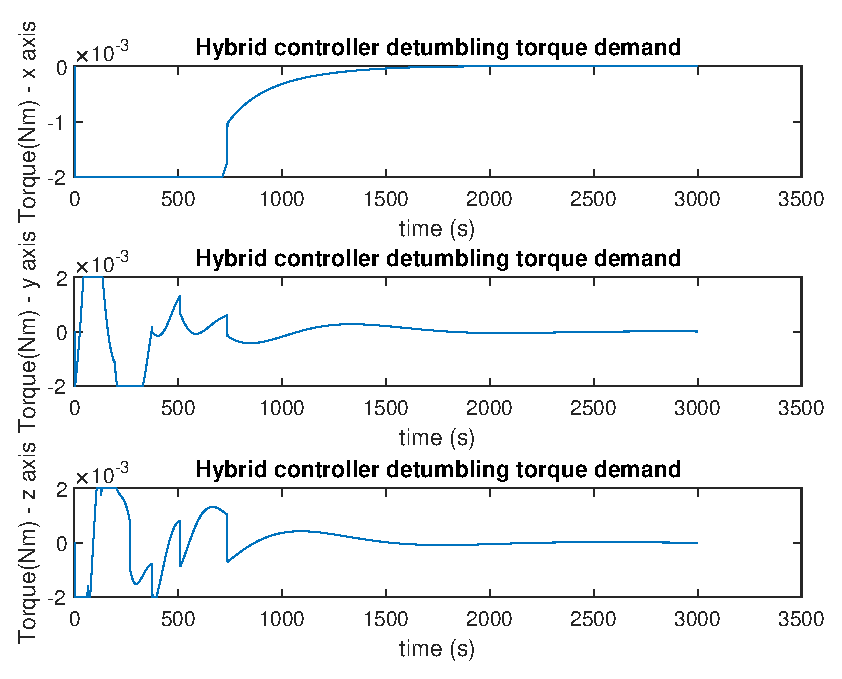
\includegraphics[width=0.7\linewidth]{figures/detumbling}
	\caption{Hybrid controller detumbling torque demand}
	\label{fig:detumbling}
\end{figure}

\begin{figure}[H]
	\centering
	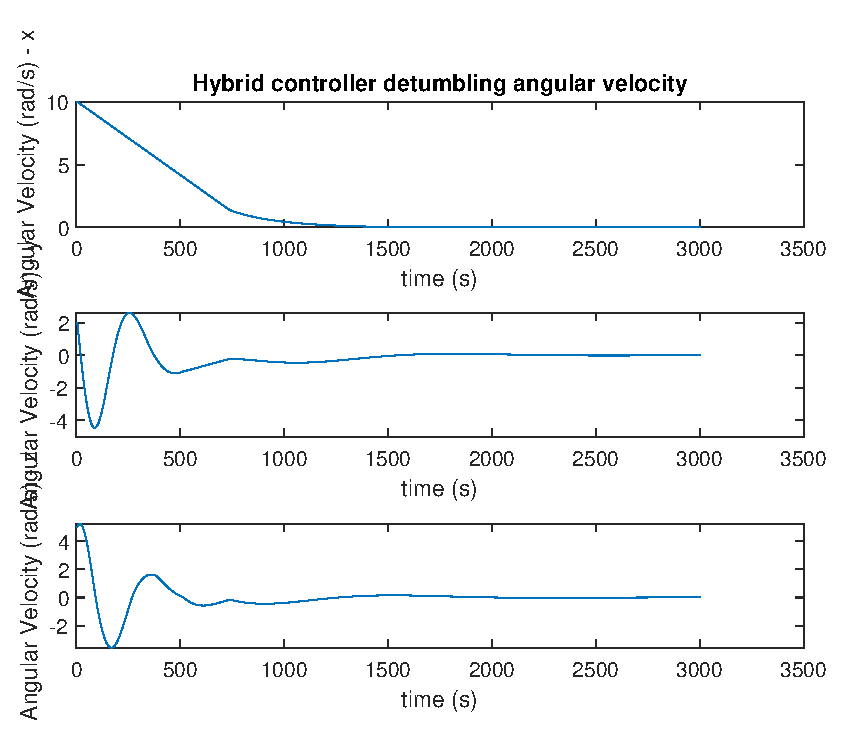
\includegraphics[width=0.7\linewidth]{figures/detumbling3}
	\caption{Hybrid controller detumbling angular velocity}
	\label{fig:omega}
\end{figure}



\subsection{Linear attitude controller} \label{sec:LC}

The operating point during nadir pointing is defined between the orbit frame and the body frame. In the operating point the angular rate between the frames should be zero $\vec{ ^s_o  \omega} = 0$ and the two frames should be aligned, thus the relative attitude quaternion is $[0 \ 0 \ 0 \ 1]^{T}$. Therefore,  $ || \vec{ {\bar{\omega}}}  ||$ is equal to the orbital angular velocity, and equation \ref{eq:lele} following \cite{Rafael} can be written as  
%
\begin{flalign}
\begin{bmatrix}
\vec{ \dot {\tilde{q}}(t) } \\
\vec{ \dot {\tilde{\omega}}(t) }
\end{bmatrix} 	
= 
\begin{bmatrix}
0 &0& 0&\frac{1}{2} &0&0& \\
0 &0& {\omega_{o}}&0 &\frac{1}{2}&0& \\
0 &-{\omega_{o}}& 0&0&0&\frac{1}{2}& \\
-2\sigma_{x} &0& 0&0 &0&0& \\
0 &2\sigma_{y}& 0&0 &0&{\omega_{o}}\sigma_{y} \\
0 &0& 0&0 &{\omega_{o}}\sigma_{z}&0& \\
\end{bmatrix} 
\begin{bmatrix}
\vec{  {\tilde{q}}(t) } \\
{  {\tilde{\vec \omega}}(t) }
\end{bmatrix} 	
-
\begin{bmatrix}
\underline{\vec 0}_{(3\times3)} \\
{\underline I_{s}^{-1}}
\end{bmatrix} 	
\vec {\tilde N_{ctrl}}
\label{eq:lelele}
\end{flalign}
%
with $\sigma_{x}= \frac{I_{y}-I_{z}}{I_{x}}$,$\sigma_{y}=\frac{I_{z}-I_{x}}{I_{y}}$,$\sigma_{z}=\frac{I_{x}-I_{y}}{I_{z}}$ and $I_{x} = 0.0017$, $I_{y}=0.0022$, $I_{z}=0.0022$ been the values of the inertia matrix and ${\omega_{o}}\approx0.0011 $ is the orbital angular rate.     
Moreover, by comparing the values of  matrix \eqref{eq:lelele} it can be seen that the value $\frac{1}{2}$ is larger compared to the other values thus \eqref{eq:lelele} can be simplified to 
\begin{flalign}
	\begin{bmatrix}
		\vec{ \dot {\tilde{q}}(t) } \\
		\vec{ \dot {\tilde{\omega}}(t) }
	\end{bmatrix} 	
	= 
	\begin{bmatrix}
		\underline{ 0}_{(3\times3)} &	\frac{1}{2} \underline{\vec 1}_{(3\times3)} \\
		\underline{ 0}_{(3\times3)} &	\underline{ 0}_{(3\times3)}
	\end{bmatrix} 
	\begin{bmatrix}
		\vec{  {\tilde{q}}(t) } \\
		{  {\tilde{\vec \omega}}(t) }
	\end{bmatrix} 	
	-
	\begin{bmatrix}
		\underline{\vec 0}_{(3\times3)} \\
		{\underline I_{s}^{-1}}
	\end{bmatrix} 	
	\vec {\tilde N_{ctrl}}
	\label{eq:lelelele}
\end{flalign}
Three equal subsystems can be derived from \eqref{eq:lelelele} as
\begin{flalign}
	\begin{bmatrix}
		\dot { \tilde {q_{i}}} \\
		\dot { \tilde { \omega_{i}}}
	\end{bmatrix} 	
	= 
	\begin{bmatrix}
		0&	\frac{1}{2}  \\
		0 &	 0
	\end{bmatrix} 
	\begin{bmatrix}
		\tilde{q_{i}}(t)  \\
		\tilde{\omega_{i}}(t) 
	\end{bmatrix} 	
	-
	\begin{bmatrix}
		0 \\
		I_{i,s}^{-1}
	\end{bmatrix} 	
	\tilde{N_{i}}
	\label{eq:subsys}
\end{flalign}
with $i = 1, 2, 3 $. The control torque was defined by the state feedback law as 
\begin{flalign}
	N_{i}^{d}	
	= 
	-
	\begin{bmatrix}
		k_{1} &	k_{2} 	
	\end{bmatrix} 
	\begin{bmatrix}
		\tilde{q_{i}}(t)  \\
		\tilde{\omega_{i}}(t) 
	\end{bmatrix} 	
	\label{eq:inputtorque}
\end{flalign}
leading to a second order closed loop system calculated as $det(s\underline{I} - (\underline{A} - \underline{BK}) )$. Identifying this with a general second order equation $s^{2}+2\zeta\omega_{n}s+\omega_{n}^{2}$, with $\zeta$ be the dumping factor which was chosen to be equal to 1 and $\omega_{n}$ the natural frequency $\omega_{n} =  \frac{2\pi}{60/0.35} $ with 60 being the chosen rise time value. The controller gains were derived as

\begin{flalign*}
	k_{1} = -2 I_{i,s} \omega_{n}^{2} 
	\label{eq:gainsl22}
\end{flalign*}
\begin{flalign*}
	k_{2} = -2\zeta I_{i,s} \omega_{n}^{2} 
	\label{eq:gainsl223}
\end{flalign*}
Since the matrix $\underline{A}$ is affine,   stability analysis was made for all the values of $ \vec{ {\bar{\omega}}}$ evaluated on the vertices of the convex polyhedron for the all values of $ \vec{ {\bar{\omega}}} $\cite{PrevPro} giving maximum eigenvalue $-0.0308$. In the figure \ref{fig:linear demand} it is seen the torque demand from the linear controller for nadir pointing reference.
\begin{figure}[H]
	\centering
	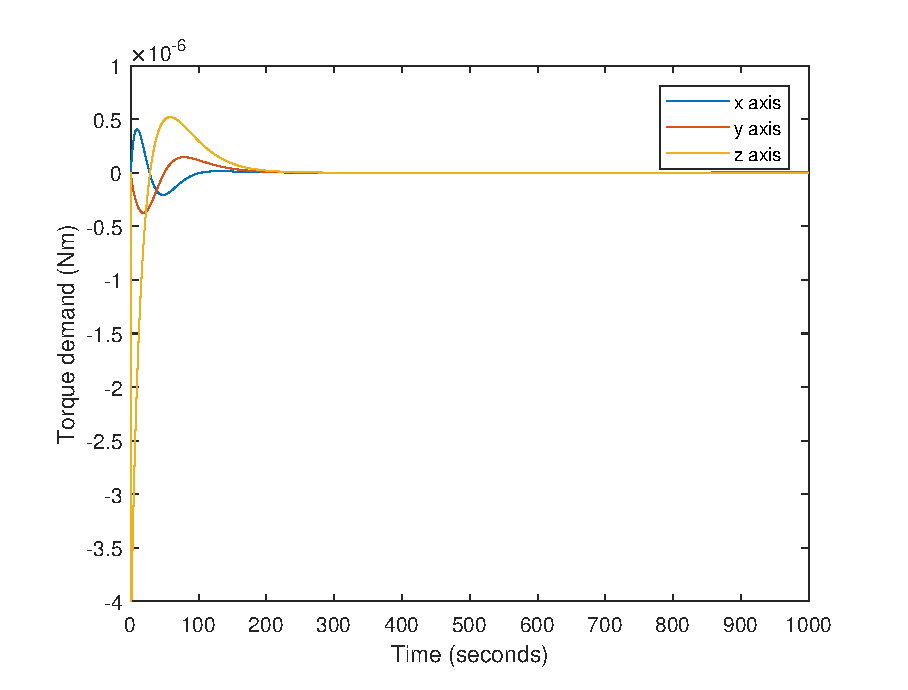
\includegraphics[width=0.7\linewidth]{figures/linear_controller_demant2}
	\caption{Linear controller Nadir pointing torque demand }
	\label{fig:linear demand}
\end{figure}
\subsection{Sliding mode control} \label{sec:SM}
As described previously, the sliding mode control scheme belongs to the class of non-linear control designs. The objective of the SMC is the design, from a geometrical point of view, of a manifold in the state space, denoted as $s$.  When the state trajectory is on the manifold ($s = 0$) it is constraint such that the behavior of the system will meet the specifications it is designed for, i.e convergence to the desired reference. In figure \ref{fig:SM} it can be seen how the states slide on the hyperplane towards origin.   

\begin{figure}[H]
	\centering
	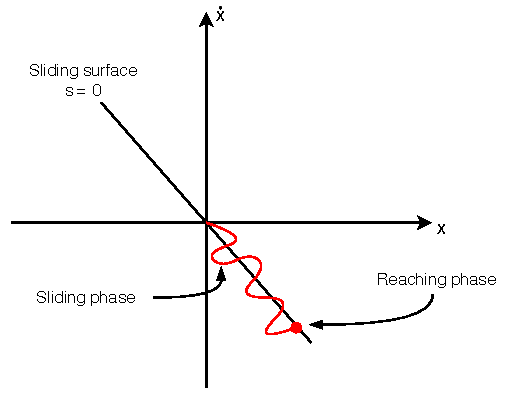
\includegraphics[width=0.5\linewidth]{figures/SM}
	\caption{Sliding mode behavior }
	\label{fig:SM}
\end{figure}
\subsection{Sliding variable design}
Small signal deviation i.e. the quaternion error can be described as
\begin{flalign}
\vec{\tilde{q}} = \vec{  \bar{q}}^{-1} \otimes \vec{ q} 
\label{eq:smallsignal22}
\end{flalign}
with $\vec{  \bar{q}}^{-1}$ be the desired reference quaternion and $\vec{ q} $ be the measured, and for the angular velocity as 
\begin{flalign}
\vec{\tilde{\omega}}  = \vec{\omega}-\vec{\bar{\omega}}  
\label{eq:smallsi4gnal4566}
\end{flalign}
with $\vec{\bar{\omega}}$ be the nominal value of the angular velocity. The sliding variable can now be written in terms of the error signals as  %\nomenclature[S]{s}{Sliding variable} and is chosen to be 
\begin{flalign}
s  = \underline{F}\vec{\tilde{q}} + \vec{\tilde{\omega}}  
\label{eq:sliding variable}
\end{flalign}
with $\underline{F} = \alpha\underline{\vec 1}_{3\times3}$ be a positive definite matrix. It can be seen that for $s=0$, the motion on the sliding surface is governed by $\vec{\tilde{\omega}} = - \alpha\vec{\tilde{q}_{1:3}}$, where $\vec{\tilde{q}_{1:3}}$ denotes the vector part of the quaternion, and $\alpha$ is chosen appropriately through trial and error to give the desired convergence for $\vec{\tilde{q}}$, leading to the desired alignment $[0 \ 0 \ 0 \ 1]^{T}$ between frames. In order to prove this, differentiation of equation \ref{eq:smallsignal22} following \cite{TH} is written as
%
\begin{flalign}
\vec{\dot{\tilde{q}}}  = \frac{1}{2}(-\vec{q_{\bar{\omega}}}\otimes\vec{\tilde{q}}+ \vec{\tilde{q}}\otimes\vec{q_{\bar{\omega}}}+\vec{\tilde{q}}\otimes\vec{q_{\tilde{\omega}}}) 
\label{eq:sliding stability}
\end{flalign}
%
with $\vec{q_{\bar{\omega}}} = \bar{\omega_{1}}i + \bar{\omega_{2}}j+\bar{\omega_{3}}k + 0$ and $\vec{q_{\tilde{\omega}}} = \tilde{\omega_{1}}i + \tilde{\omega_{2}}j+\tilde{\omega_{3}}k + 0$.
From equation \ref{eq:sliding stability} the real part of the quaternion error can be written as 
%
\begin{flalign}
\dot{\tilde{q_{4}}}  = -\frac{1}{2} \vec{\tilde{\omega}}  \vec{\tilde{q}_{1:3}} = \frac{\alpha}{2} \rVert \vec{\tilde{q}_{1:3}} \rVert^{2} = \frac{\alpha}{2}(1 -\tilde{q_{4}}^{2})
\label{eq:sliding realpart}
\end{flalign}
%
It can be seen that $\vec{\tilde{q}} \longrightarrow [0\ 0\ 0\ 1]^{T}$ with a desired rate given by $\alpha$. Figure \ref{fig:quaterror} showing the $\vec{\tilde{q}}$ converging with rate given by $\alpha = 0.035$

\begin{figure}[H]
	\centering
	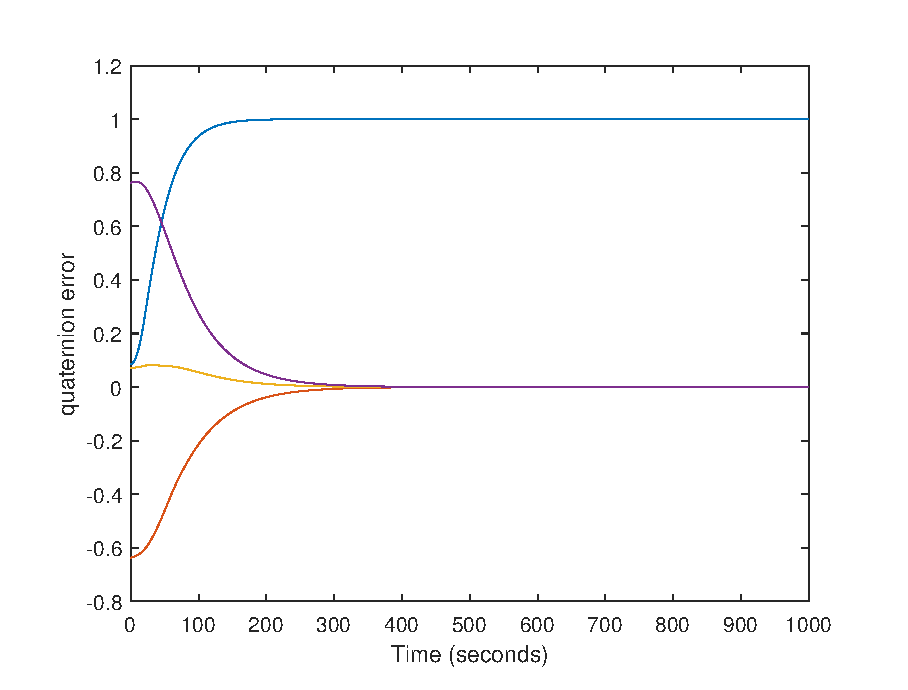
\includegraphics[width=0.7\linewidth]{figures/quaternion_error}
	\caption{Shows the quaternion error converging with $\alpha = 0.035$ }
	\label{fig:quaterror}
\end{figure}
\subsection{Sliding condition - Control law}
The variable $s$ can be driven to 0 by making use of a Lyapunov candidate function as
\begin{flalign}
V  = \frac{1}{2} \vec{s}^{T}\vec{s} 
\label{eq:sliding variable333}
\end{flalign} 
and in order to prove stability around $s=0$ a necessary condition is $\dot{V} < 0 $ for each $s\neq0$. The time derivative of equation \ref{eq:sliding variable333} is written as
\begin{flalign}
\dot{V}  = \frac{1}{2}( \dot{\vec{s}^{T}}\vec{s}+\vec{s}^{T}\dot{\vec{s}}) 
\label{eq:sliding variable33333}
\end{flalign}
showing that $\vec{s}^{T}\dot{\vec{s}} < 0 $ $\forall s\neq0$ the condition may be satisfied.
Substituting equation \ref{eq:sliding variable} is obtained
\begin{flalign}
\dot{V}  = \vec{s}^{T}\dot{\vec{s}}  = \vec{s}^{T} (\underline{F}{\vec{\dot{\tilde{q}}}} + {\vec{\dot{\tilde{\omega}}}}) 
\label{eq:e33333}
\end{flalign}
and thus replacing the dynamic equation \ref{eq:seom}, equation \ref{eq:e33333} may be written as 


\begin{flalign}
\dot{V}  = \vec{s}^{T}\underline{I}_{s}^{-1}(-\underline{{\omega}}^\times\underline{I}_{s}\vec{\omega}-\underline{{\omega}}^\times\vec{h_{rw}}+\vec{N_{rw}^{d}}+\vec{N_{mt}}+\vec{N_{dis}} - \underline{I}_{s}\dot{\bar{\omega}} +\underline{I}_{s}\underline{F}{\vec{\dot{\tilde{q}}}} ) 
\label{eq:444444}
\end{flalign}
designing the control as
\begin{flalign}
\vec{N_{rw}^{d}}  = \underline{{\omega}}^\times\underline{I}_{s}\vec{\omega}+\underline{{\omega}}^\times\vec{h_{rw}} + \underline{I}_{s}\dot{\omega} -\underline{I}_{s}\underline{F}{\vec{\dot{\tilde{q}}}}-\underline{I}_{s}\lambda sign(\vec{s})  ) 
\label{eq:555555}
\end{flalign}

equation \ref{eq:444444} is written as
\begin{flalign}
\dot{V}  = -\vec{s}^{T}(-{\vec{\dot{\tilde{\omega}}}} + \lambda sign(\vec{s}) -\vec{N_{mt}}-\vec{N_{dist}} ) 
\label{eq:stability}
\end{flalign}
Eventually, it can be seen that choosing $\lambda > \lVert{\vec{\dot{\tilde{\omega}}_{max}}} \rVert + \lVert \vec{N_{mt}} \rVert + \lVert \vec{N_{dist}} \rVert $ the condition $\dot{V} < 0 $ is satisfied. Sign function presents chattering around the manifold which is undesirable, thus the sign function is replaced with the hyperbolic tangent function $tanh$ which is smoother. In the figure \ref{fig:slidingtorque} is depicted the torque demand the sliding mode controller outputs. 
\begin{figure}[H]
	\centering
	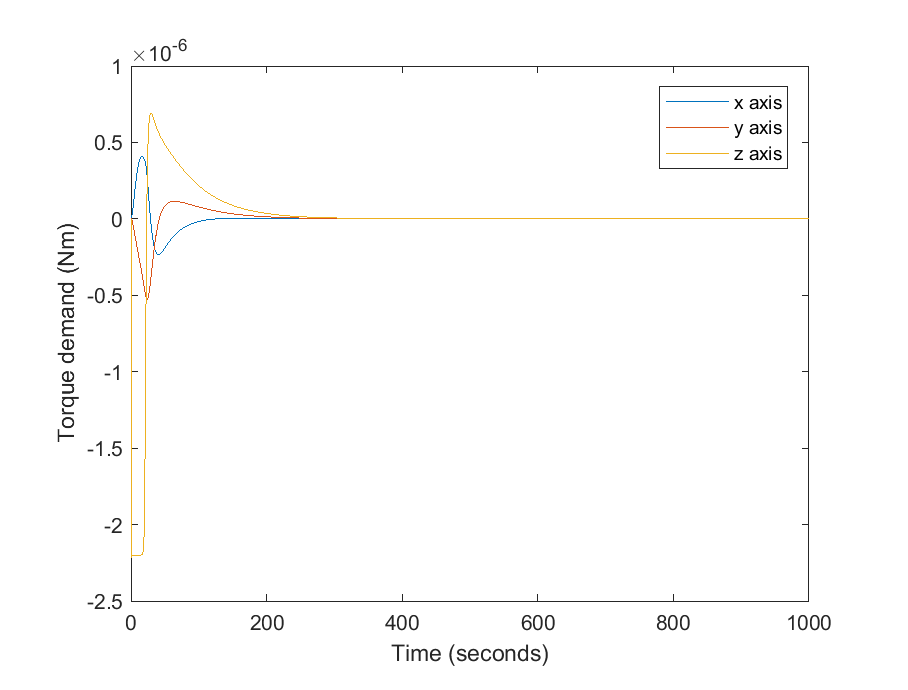
\includegraphics[width=0.7\linewidth]{figures/SMC_tor2}
	\caption{Sliding Mode controller nadir pointing torque demand }
	\label{fig:slidingtorque}
\end{figure} 


\chapter{Fault  Analysis and Detection}

INTRO \todo{write the intro}

\section{Fault Detection}
\textit{In this chapter, probable faults in the system are examined using a  Failure Mode and Effects Analysis (FMEA). Next, in order to find how probable a fault will happen and the effect of it, the severity and occurrance (SO)  of faults is analyzed. It was decided that the fault analysis will be carry out only for the actuators (magnetorquers and momentum wheels).}

\nomenclature[A]{\textbf{FMEA}}{Failure Mode and Effects Analysis}
\nomenclature[A]{\textbf{SO}}{Severity and Occurrance}
\nomenclature[A]{\textbf{FDI}}{Fault Detection and Isolation}
\nomenclature[S]{$\vec{{F}_{MT}}$}{The fault vector for the magnetorqers}
\nomenclature[S]{$\vec{{F}_{RW}}$}{The fault vector for the reaction wheels}

A fault in a system can be seen as a sudden shift in the system functionality, nevertheless, it might not mean a total shutdown of the system. One way to see it is as a disturbance in the system, that might cause performance loss or serious deterioration to the system. On the other hand, a failure can be understood as a total shutdown of the system component. 

In \figref{fig:1} a fault tolerant system is shown, which contains an autonomous supervisor that has the ability to switch between various controllers taking into account the type of fault that a component has. The spacecraft block illustrated in the picture is composed of a plant, actuators and sensors and is monitored by the fault detection and isolation  (FDI) system, which include detectors that will feed informations to the supervisor in the eventuality of a fault. Based on the information received, the supervisor will establish if a fault occurred or not and in case of a fault the effectors will handle it. Figure \ref{fig:2} shows the procedure of how faults are handled with varius methods. The first step in Fault Analysis is fault modelling which uses a procedure called FMEA.
\begin{table}[H]
	\begin{minipage}[b]{0.49\linewidth}
		\centering
		\begin{figure}[H]
			\centering
			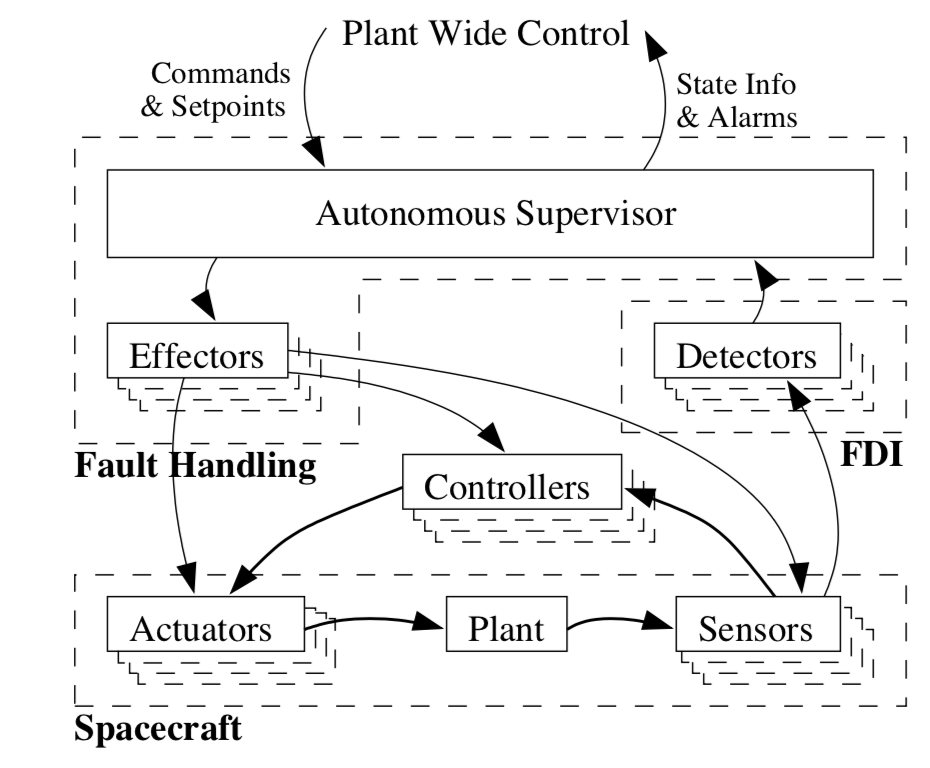
\includegraphics[width=1\linewidth]{figures/FTC}
			\caption{Fault tolerant system architecture \cite{FTJ}}
			\label{fig:1}
		\end{figure}
	\end{minipage}\hfill
	\begin{minipage}[b]{0.49\linewidth}
		\centering
		\begin{figure}[H]
			\centering
			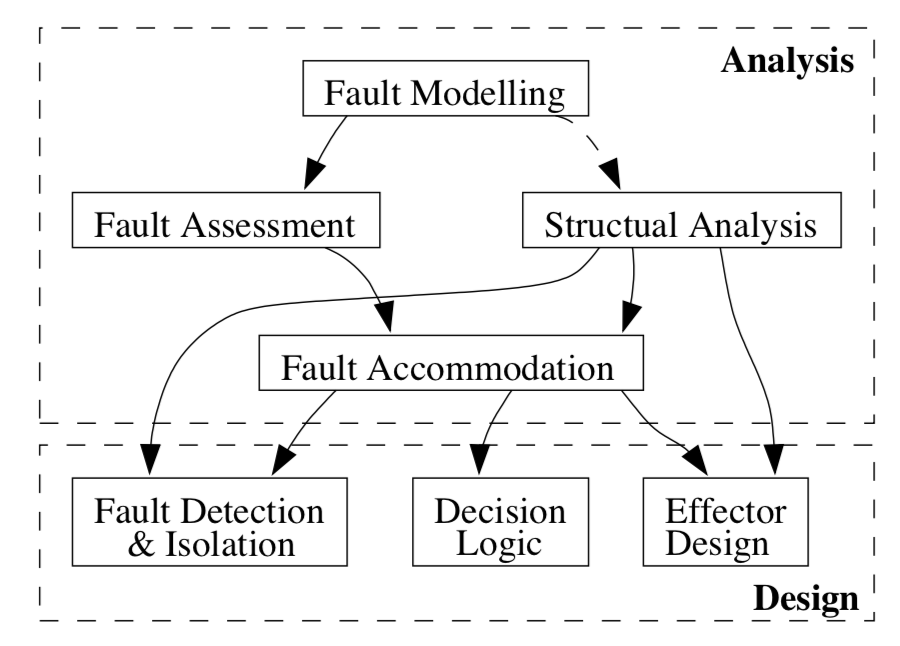
\includegraphics[width=1\linewidth]{figures/FTC_2}
			\caption{ }
			\label{fig:2}
		\end{figure}
	\end{minipage}
\end{table}
\subsection{Failure Mode and Effects Analysis}

\todo{perhaps simplify }

A FMEA analysis which is a bottom-up analysis method is performed for the components of the satellite. The main goal of FMEA is to identify possible faults and their effects on components. In order to evaluate how faults are propagated through the system, a FMEA scheme is constructed.
Another aspect of FMEA analysis is that, the severity of a fault can be determined, which will offer the opportunity to prioritize the faults by severity and in this way focus on the important faults.

In order to control the attitude of the satellite, two types of actuators are used: magnetorquers and reaction wheels. Potential faults are gather into a table which describes the effect and cause, while the satellite is orbiting.
\subsubsection{Magnetorquers}
\begin{table}[H]
	\centering
	\label{my-label}
	\begin{tabular}{|l|l|l|}
		\hline
		\multicolumn{3}{|c|}{\textit{\textbf{Magnetorquers}}}                                          \\ \hline
		\multicolumn{3}{|c|}{Creates a magnetic field that interacts with Earth's magnetic field}                     \\ \hline
		\textbf{Reference} & \textbf{Failure Effect} & \textbf{Failure Cause}                          \\ \hline
		$MT1$                 & Low magnetic field  & \begin{tabular}[c]{@{}l@{}}1) Broken wire or bad soldering\\ 2) Component burned\end{tabular} \\ \hline
		$MT2$                 & Maximum magnetic field power  & Short circuit to the power voltage   \\ \hline
		$MT3$                 & Wrong direction of the magnetic field & \begin{tabular}[c]{@{}l@{}} 1) Misalignment of the magnetorquer\\ 2) Short circuit of some parts of the \\ torquer to the power voltage \end{tabular} \\ \hline
		$MT4$                 & Wrong  power of the magnetic field                 & Floating supplay voltage                                            \\ \hline
	\end{tabular}
	\caption{Potential faults in the magnetorquers}
\end{table}
Description of faults in the magnetorquers: 

$\mathcal{F}_{MT1}$: 
The coil it might have a broken wire or a bad soldering inside, that will lead to a poor generation of magnetic field from the magnetorqers. On the other hand, a component could be burned due to a fluctuation in the current. \todo{voltage regulator is the reason}

$\mathcal{F}_{MT2}$: 
With a short circuit in the power supply, a maximum magnetic field power is expected.

$\mathcal{F}_{MT3}$:
A misalignment of the magnetorquer  due to transportation or a sudden shift during the launch, could affect the direction of the magnetic field.

$\mathcal{F}_{MT4}$:  
A variable supply voltage that could mean a positive or negative operation will end up with an error power of the magnetic field.

The fault vector for the magnetorqers is constructed as follows:

$\mathcal {\vec{{F}_{MT}}}$ = [ \ $\mathcal{F}_{MT1}$ \ $\mathcal{F}_{MT2}$ \ $\mathcal{F}_{MT3}$ \ $\mathcal{F}_{MT4}$ ]$^ \mathsf{T}$
\subsubsection{Reaction wheels}
\begin{table}[H]
	\centering
	\label{my-label}
	\begin{tabular}{|l|l|l|}
		\hline
		\multicolumn{3}{|c|}{\textit{\textbf{Reaction wheels}}}                                          \\ \hline
		\multicolumn{3}{|c|}{Produces a torque about the satellite COM in order to rotate it }                     \\ \hline
		\textbf{Reference} & \textbf{Failure Effect} & \textbf{Failure Cause}                          \\ \hline
		$RW1$                & Faulty orientation & \begin{tabular}[c]{@{}l@{}} Shifting of the flywheel  \\   \end{tabular} \\ \hline
		$RW2$                & Unable to control the rotation   & A short-circuit in the power supply  \\ \hline
		$RW3$                & Low power received& \begin{tabular}[c]{@{}l@{}} Short circuit to the ground\\  \end{tabular} \\ \hline
		$RW4$                & No torque received  &  A fault in windings    \\ \hline
	\end{tabular}
	\caption{Potential faults in the reaction wheels}
\end{table}
Description of faults in the reaction wheels: 

$\mathcal{F}_{RW1}$: 
A displacement of the flywheel throughout launch or transportation could result in a error in the orientation that might alter the angular velocity of the satellite.

$\mathcal{F}_{RW2}$: 
A short-circuit in the power supply could influence the rotation of the flywheel, by having a low or maximum rotation, which will end up with a low or maximum power.

$\mathcal{F}_{RW3}$:
A short circuit to the ground due to a borken wire or bad soldering will result in low power generation, that could influence the rotation of the flywheel.

$\mathcal{F}_{RW4}$:  
Due to a fault in the windings, the flywheel will not be able to rotate, therefore, no torque will be received.

The fault vector for the reaction wheels is constructed as follows:

$\mathcal {\vec{{F}_{RW}}}$ = [ \ $\mathcal{F}_{RW1}$ \ $\mathcal{F}_{RW2}$ \ $\mathcal{F}_{RW3}$ \ $\mathcal{F}_{RW4}$ ]$^ \mathsf{T}$
\subsubsection{Severity and occurrence evaluation}
The next step into Fault Analysis is the Fault Assessment that involves a Severity Occurrence analysis
To investigate the faults that have the biggest rate of occurrence, the severity of the effects of failures and the probability of occurrence is determined based on the faults from FMEA. This procedure describes how to each fault receives a severity index \nomenclature[A]{\textbf{SI}}{Severity Index} (SI) and an occurrence index \nomenclature[A]{\textbf{OI}}{Occurrence Index} (OI). A table containing the serverity and occurrence for magnetorquers is shown as follows:
\begin{table}[H]
	\centering
	\label{11}
	\begin{tabular}{|l|l|l|l|}
		\hline
		\multicolumn{4}{|c|}{\textit{Magnetorquer}}                                                                                         \\ \hline
		Reference & Severity & Occurrence                                          & SO Index                                      \\ \hline
		$MT1$     & 7        & \begin{tabular}[c]{@{}l@{}} 5\\  4\end{tabular} & \begin{tabular}[c]{@{}l@{}} 35\\ 28\end{tabular} \\ \hline
		$MT2$       & 10       & 3       & 30                \\ \hline
		$MT3$       & 3        & \begin{tabular}[c]{@{}l@{}}2\\ 1\end{tabular} & \begin{tabular}[c]{@{}l@{}}6\\ 3\end{tabular} \\ \hline
		$MT4$       & 4        & 6                   & 24                  \\ \hline
	\end{tabular}
\caption{SO for magnetorquer}
\end{table}
The same procedure is done for momentum wheels as follows:
\begin{table}[H]
	\centering
	\label{12}
	\begin{tabular}{|l|l|l|l|}
		\hline
		\multicolumn{4}{|c|}{\textit{Reaction wheels}}                                                                                         \\ \hline
		Reference & Severity & Occurrence                                          & SO Index                                      \\ \hline
		$RW1$      & 1        & \begin{tabular}[c]{@{}l@{}}7\\ \end{tabular} & \begin{tabular}[c]{@{}l@{}}7\\ \end{tabular} \\ \hline
		$RW2$        & 1        & 4             & 4                                         \\ \hline
		$RW3$        & 2        & \begin{tabular}[c]{@{}l@{}}3\\\end{tabular} & \begin{tabular}[c]{@{}l@{}}8\\ \end{tabular} \\ \hline
		$RW4$        & 4        & 2     & 8               \\ \hline
	\end{tabular}
	\caption{SO for momentum wheels}
\end{table}

The severity index is computed using the following formula:
\begin{flalign}
	SO_{index} = severity \cdot occurrence
	\label{eq:ec1}
\end{flalign} 

\subsubsection{Fault propagation analysis}
In order to observe how faults are propagated through the system and the effect of these faults, a FMEA scheme is constructed. Further computation will be on the appendix.

\chapter{Fault Detection}

Fault detection deals with detecting system discrepancies, abnormal behaviour. It is the first step towards handling faults. It doesn't necessarily identify the source of the fault, just establishes the fact that a fault has occurred in the system.


\section{Motors fault detection}

\label{sec:structural}
\subsection{Structural Analysis}
Structural analysis studies the interrelation between parameters and variables of the system using constraints between them. It distinguishes known and unknown variables, according to whether they can be measured in the system or not. Then the unknown variables are expressed using the known ones according to the constraints. Structural analysis based residual signal require that unknown variables can be expressed redundantly. One of the constraints is used to express the unknown, the other to verify it. If there's a mismatch between the two, a fault is detected.

In case of fault detection in sensors, one constraint is between the measured and the actual values of a variable. In case of a sensor fault, there can be a considerable difference between the measured and the actual value of a variable.

Assumes that only one fault occurs at any given time, so faults cannot mutually neutralize each other. 

The constraints being used to detect faults in the motor are:

\ref{sec:motor} \todo{reference motor section properly}


\begin{equation}
V_a = R_a * i + k_e \omega
\end{equation}

$L_a$ is negligible

\begin{equation}
 k_{t}i  =J\dfrac{d\omega}{dt} + b\omega
\end{equation}

\begin{equation}
\tau = k_t i
\end{equation}

$d_1(\omega, \dot{\omega})$


\subsection{Alternative method for identifying reaction wheel fault}

With enough computational power the faulty reaction wheel can be detected through the calculated reaction wheel output torque, assuming only one reaction wheel is faulty. It is done by calculating the difference between 3D torque demand and actual 3D torque output. 

\begin{equation}
\vec{N}_{rw} = \underline{I}_s \dot{\vec{\omega}}  + \vec{\omega} \times \vec{h_{rw}} - \vec{N_{mt}} - \vec{N_{dist}}
\end{equation}

Then the difference between torque demand and torque output is calculated. The reaction wheel that has the most similar axis orientation to the torque difference is deemed as faulty.

\begin{equation}
\vec{N}_{rw}^{demand} - \vec{N}_{rw}^{actual} = 
\vec{N}_{rw}^{diff}
\end{equation}

\begin{equation}
 \pm \vec{N}_{rw}^{diff}  \stackrel{?}{\approx} \vec{axis} 
\end{equation}


\todo{mention unit vector notation, decide notation for axis, express axis according to q}

Note: the lag for torque change and wheel saturation has to be taken into account separately, as those don't count as faults. 
Thresholds should be applied.

\section{Magneto torquers  fault detection}

\subsection{Unknown Input Observer (UIO)}

Uncertainties and modeling errors may cause discrepancies between the actual system and the descriptor mathematical model. Linearization and simplifications which make the system more manageable may lead also to uncertainties. All these uncertainties can have an effect on the system dynamic behavior through the input signals.   
A residual, fault indicator, based on observer design can be robust regarding the unknown input signals by making the effect of unknown inputs(UI) insensitive to the residual and thus making possible to maximize the detectability of a fault. 
Following \cite{UIO}     
\chapter{Acceptance test} \label{chap:acceptanceTest}

The system is tested to see if it fulfills the requirements put up (\chapref{chap:requirements}).

Nadir pointing capability is tested by turning on the linear attitude controller of a satellite with initial attitude and angular velocity deviating from the reference. After reducing the initial error, the tracking error stays below $1^o$, as shown in figure 9.1.

\begin{figure}[H]
	\centering
	%	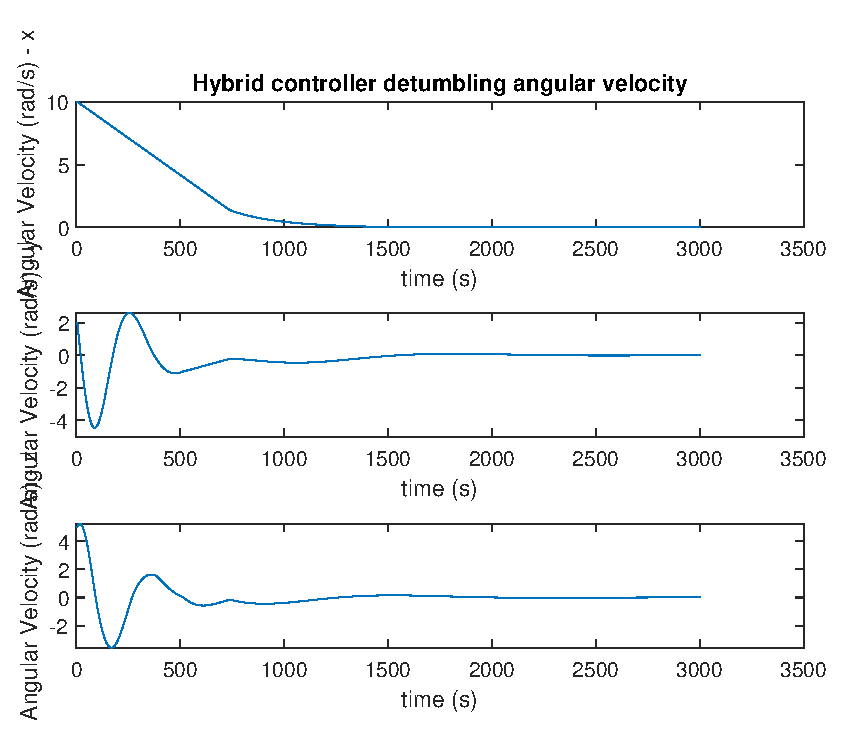
\includegraphics[width=0.7\linewidth]{figures/detumbling3}
	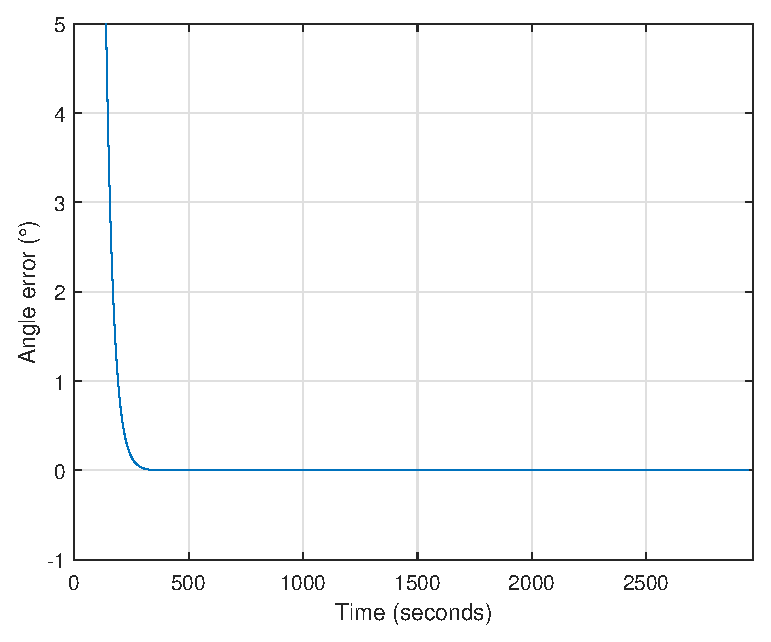
\includegraphics[width=0.7\linewidth]{figures/angle_error}
	\caption{Tracking error during nadir pointing}
	\label{fig:angle_error}
\end{figure}

Earth station tracking is  tested in a scenario where the satellite flies right over the station. This is the closest the satellite in orbit can get to the Earth station, leading to maximum torque demand. The tracking error is kept below  $1^o$, with error peaks appearing during flyover. Figures \ref{fig:angle_error2} and \ref{fig:torque_stationTrack} present the tracking error and torque demand arising during station tracking.

\begin{figure}[H]
	\centering
	%	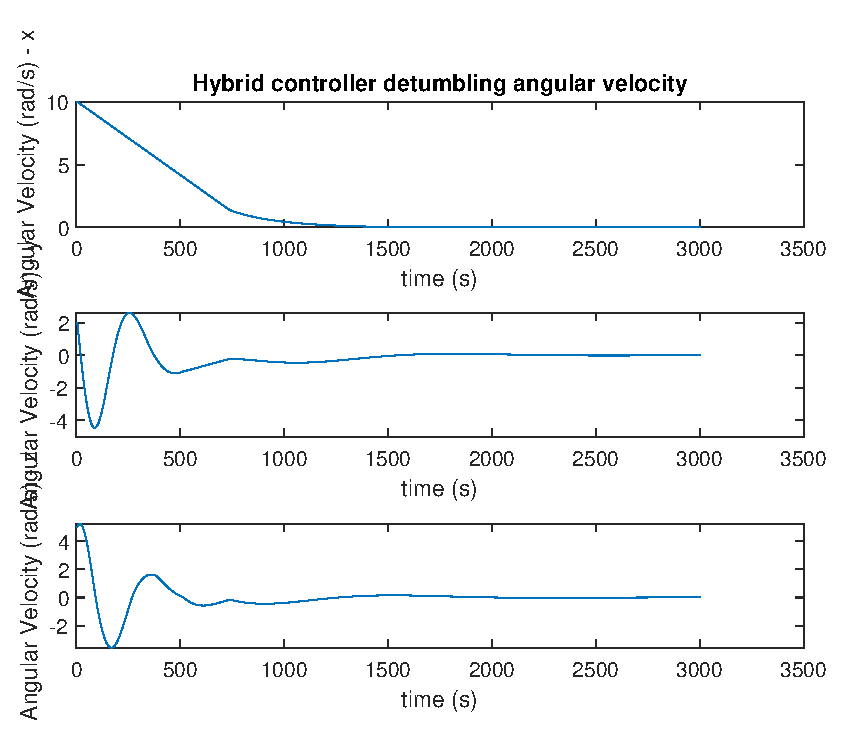
\includegraphics[width=0.7\linewidth]{figures/detumbling3}
	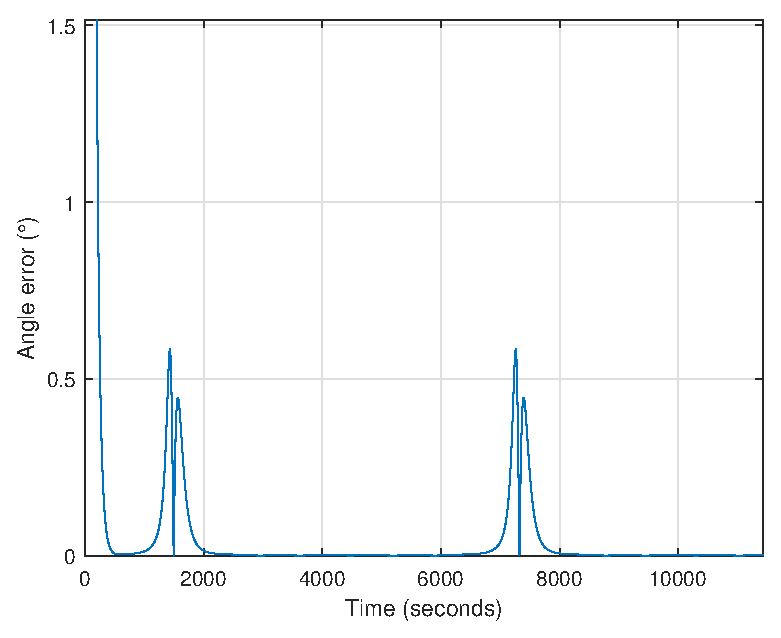
\includegraphics[width=0.7\linewidth]{figures/angle_error_stationTrack}
	\caption{Tracking error during Earth station pointing. The satellite flies over the station.}
	\label{fig:angle_error2}
\end{figure}


\begin{figure}[H]
	\centering
	%	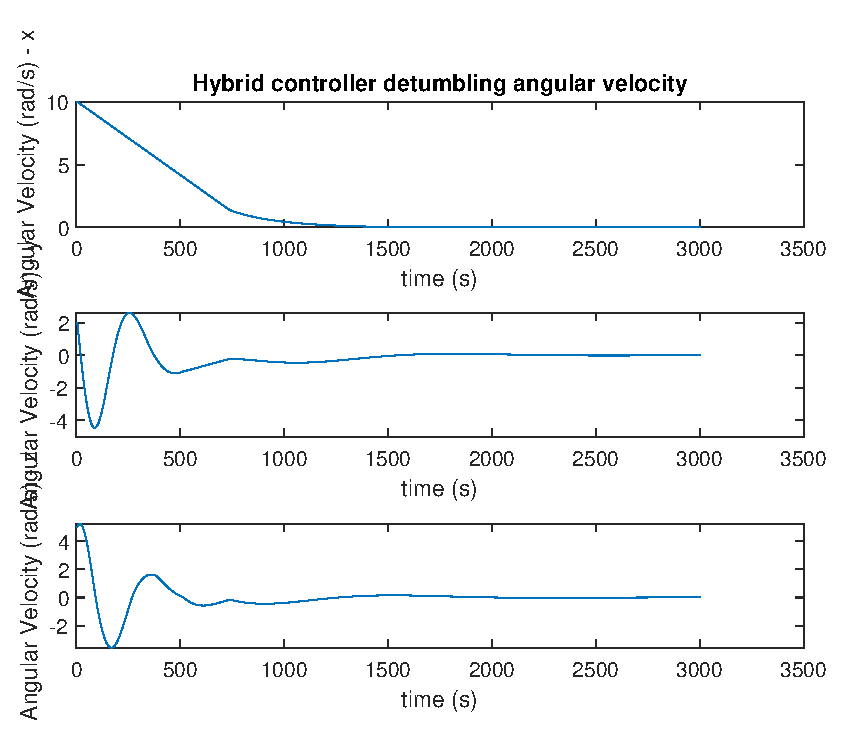
\includegraphics[width=0.7\linewidth]{figures/detumbling3}
	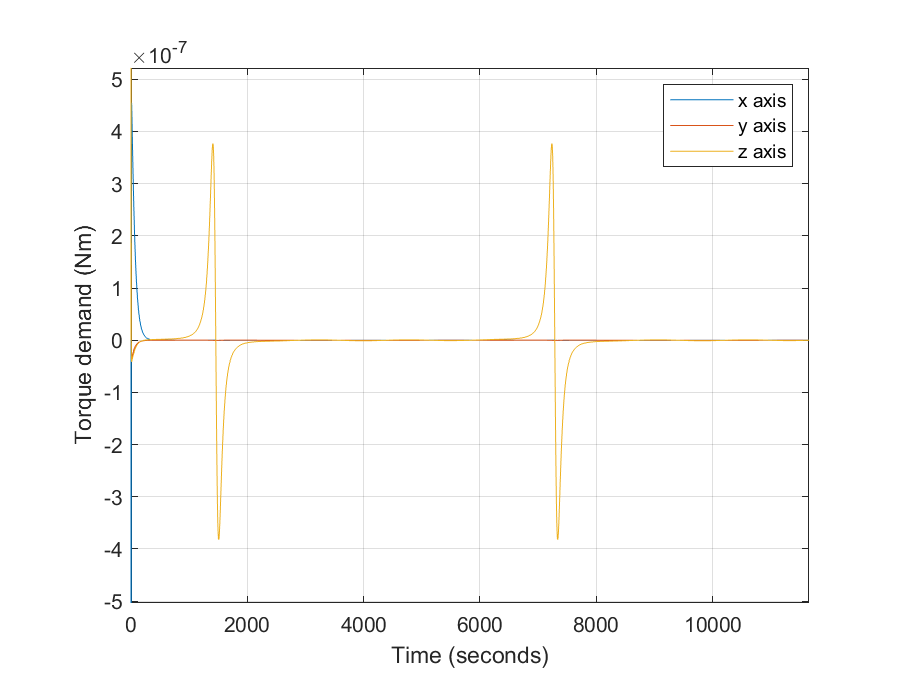
\includegraphics[width=0.7\linewidth]{figures/torque_stationTrack}
	\caption{Torque demand $\vec{u}$ during Earth station pointing. The satellite flies over the station.}
	\label{fig:torque_stationTrack}
\end{figure}

\begin{figure}[H]
	\centering
	%	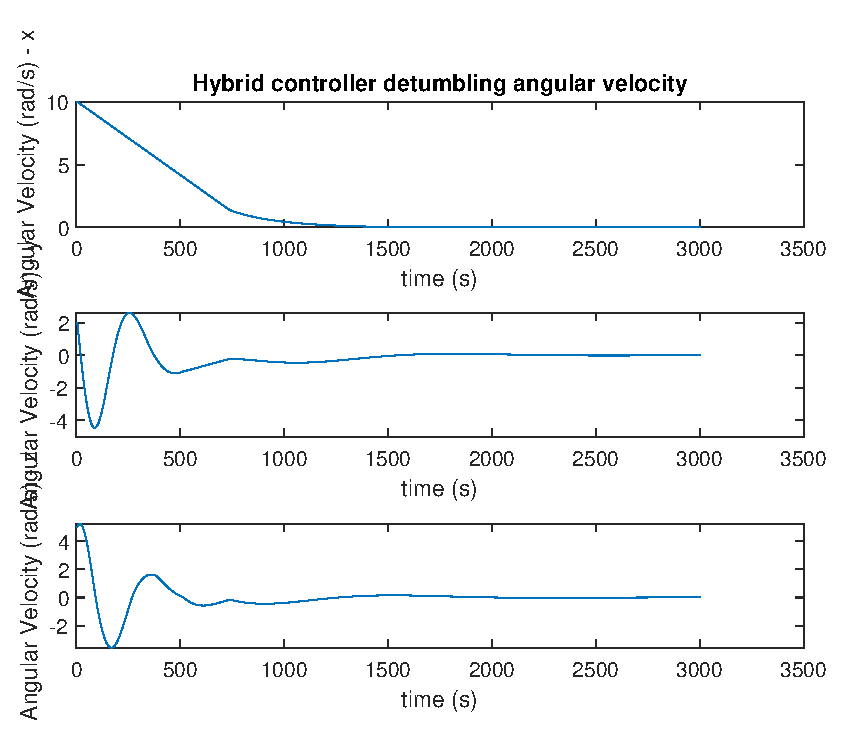
\includegraphics[width=0.7\linewidth]{figures/detumbling3}
	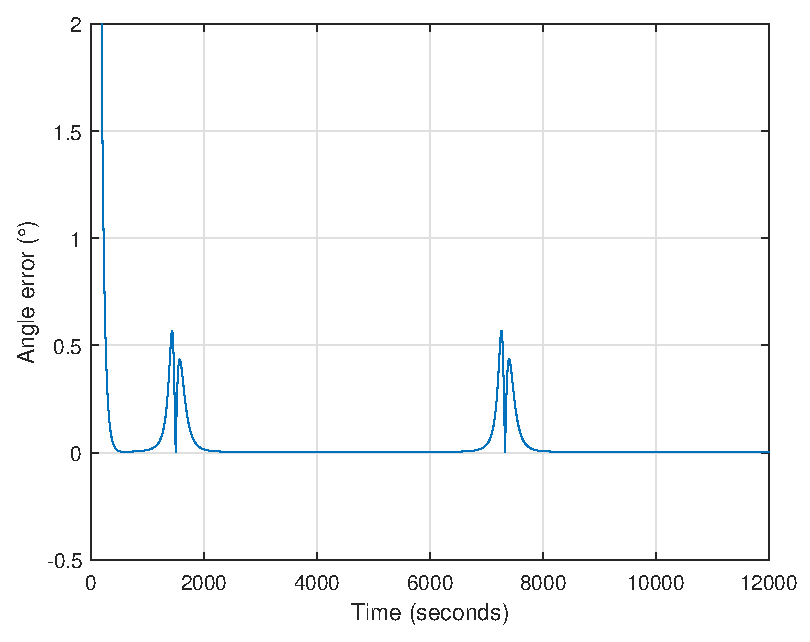
\includegraphics[width=0.7\linewidth]{figures/faultyangerror}
	\caption{Tracking error during Earth station pointing using the linear controller. The satellite flies over the station. The 3rd reaction wheel is faulty and switched off.}
	\label{fig:angle_error2}
\end{figure}


%\subsection{1. The formation shall be able to maintain a given angle within 45$^{\circ}$.}
%The

\chapter{Conclusion}
The overall objective of this project was to consider several satellites flying in formation with the purpose of pointing towards a target. In order to reach this goal, two controllers were designed: one for controlling the angle between satellites using the drag force and another one for attitude control in order to be able to rotate the satellite to the desired orientation.

First, for designing a controller for the angle, the relative dynamics between two satellites are analyzed. Therefore, an LQR controller is implemented to control the angle between two satellites. The simulations showed that the LQR performed properly. Additionally, two algorithms for formation control are designed, a global and distributed algorithm. Both algorithms are working as intended, where the angles between neighbour satellites converged to the desired angle of 45$^{\circ}$, with the mention that in the distributed algorithm case the convergence rate will be slower compared with the global algorithm.

Afterwards, two control methods to obtain the desired orientation of the satellite has been implemented. The first method is a state feedback which is a linear control method. For implementing this controller the equation of motion need to be linearized. The second method is using a non-linear control method called sliding mode control. The results from sliding mode control showed that the error quaternion converged better compared to state feedback control, but in this case, the state feedback is deemed to be more suitable. Besides, the sliding mode convergence is better, but due to the fact that the control law is more complex, the satellite controller will need more computation time. 

In conclusion, some acceptance tests have been made to establish that the requirements accomplished. 



%%% Bibliography %%%
%---------- Appendix Below ----------------------------------------
\appendix
\chapter{Quaternions } \label{chap:A}
This appendix is based on sources from \cite{SADC} and \cite{Kui}.

There are several possible mathematical representations for rotation. In physics, rotation matrices, Euler angles (eg. pitch-roll-yaw) and quaternions. In satellite engineering, quaternions are the preferred representations, since they are more compact than rotation matrices and lack singularities.

Quaternions include four values, three of them represent a vector \textbf{$\epsilon$}, the fourth a scalar $\eta$. 
\begin{equation}
\textbf{q} =
\left[ 
\begin{array}{cccc}
q_1 \\
q_2 \\  
q_3 \\
q_4 
\end{array}
\right] 
= 
\left[ 
\begin{array}{cccc}
\textbf{$\epsilon$} \\
\eta
\end{array}
\right] 
\end{equation}
A rotation with $\Phi$ around the unit vector can be described according to Euler's formula.
\begin{equation}
\vec q = e^{\frac{\Phi}{2} (e_1 \textbf{i}+ e_2 \textbf{j} + e_3 \textbf{k} + e_4)} = \cos \frac{\Phi}{2} + (e_1 \textbf{i}+ e_2 \textbf{j} + e_3 \textbf{k} +e_4) \sin \frac{\Phi}{2}
\end{equation}

Consequently 
\begin{equation}
\textbf{q} =
\left[ 
\begin{array}{cccc}
q_1 \\
q_2 \\  
q_3 \\
q_4 
\end{array}
\right] 
= 
\left[ 
\begin{array}{cccc}
e_1  \sin \frac{\Phi}{2} \\
e_2  \sin \frac{\Phi}{2} \\  
e_3  \sin \frac{\Phi}{2} \\
\cos \frac{\Phi}{2} 
\end{array}
\right] 
\end{equation}

\subsection{Quaternion multiplication}
Let \textbf{q} represent the unit length rotation axis, with \textbf{i}, \textbf{j}, \textbf{k} being the base vectors in euclidean space and $e_4$ as the scalar part: 
\begin{equation}
\textbf{q} = q_1 \textbf{i}  + q_2 \textbf{j} + q_3 \textbf{k} + q_4
\end{equation}

where $\textbf{i}, \textbf{j}, \textbf{k}$ represent the hyper imaginary parts and satisfying the rules introduced by Hamilton:
\begin{align*}
	\begin{split}
		\vec {i^{2}} &=  \vec {j^{2}}  = \vec {k^{2}} = -1 \\
		{\vec {i}} {\vec {j}} &= - {\vec {j}} {\vec {i}} = \vec k \\
		{\vec {j}} {\vec {k}} &= - {\vec {k}} {\vec {j}} = \vec i \\
		{\vec {k}} {\vec {i}} &= - {\vec {i}} {\vec {k}} = \vec j 
	\end{split}
\end{align*}
Next a product of two quaternions $\vec q_A$ and $\vec q_B$ is illustrated:
\begin{flalign}
	\vec q_C = \vec q_A \otimes \vec q_B = ( q_{A_{1}} \vec i + q_{A_{2}} \vec j + q_{A_{3}} \vec k + q_{A_{4}}) \otimes ( q_{B_{1}} \vec i + q_{B_{2}} \vec j + q_{B_{3}} \vec k + q_{B_{4}})
		\label{eq:quat}
\end{flalign}
After rearranging terms and using the rules above, equation \ref{eq:quat} becomes:
\begin{flalign}
\vec q_C &= ( q_{A_{1}} q_{B_{4}} + q_{A_{2}}q_{B_{3}} - q_{A_{3}}q_{B_{2}}  + q_{A_{4}} q_{B_{1}}) \vec i + \\ 
&+( - q_{A_{1}} q_{B_{3}} + q_{A_{2}}q_{B_{4}} - q_{A_{3}}q_{B_{1}}  + q_{A_{4}} q_{B_{2}}) \vec j + \\
&+( q_{A_{1}} q_{B_{2}} - q_{A_{2}}q_{B_{1}} - q_{A_{3}}q_{B_{4}}  + q_{A_{4}} q_{B_{3}}) \vec k + \\
&+ (- q_{A_{1}} q_{B_{1}} - q_{A_{2}}q_{B_{2}} - q_{A_{3}}q_{B_{3}}  + q_{A_{4}} q_{B_{4}}) 
	\label{eq:quat2}
\end{flalign}
The product quaternion can be expressed in a matrix form:
\begin{flalign}   
	\begin{bmatrix}
		 q_{C_{1}} \\
		 q_{C_{2}}  \\ 
		 q_{C_{3}}  \\ 
		 q_{C_{4}}  \\ 
	\end{bmatrix} 
	&= 
		\underbrace{
	\begin{bmatrix}
		q_{A_{4}}& q_{A_{3}}& -q_{A_{2}}&q_{A_{1}}&\\
		-q_{A_{3}}& q_{A_{4}}& q_{A_{1}}&q_{A_{2}}&\\
		q_{A_{2}}& -q_{A_{1}}& q_{A_{4}}&q_{A_{3}}&\\
		-q_{A_{1}}& -q_{A_{2}}& -q_{A_{3}}&q_{A_{4}}&\\
	\end{bmatrix} 
}_{\underline{C}_A}
	\begin{bmatrix}
    q_{B_{1}} \\
	q_{B_{2}}  \\ 
	q_{B_{3}}  \\ 
	q_{B_{4}}  \\  
	\end{bmatrix} 	
	\label{eq:sfgdm}
\end{flalign}
A skew-symmetric matrix is given as $\underline{S}(\vec q)^\times$ and defined as
\begin{flalign}   
	\underline{S}(\vec q)^\times = 
	\begin{bmatrix}
		 0 & - q_{A_{3}}  & q_{A_{2}}\\
		 q_{A_{3}}&  0  & - q_{A_{1}} \\ 
		- q_{A_{2}}&  q_{A_{1}}  & 0 \\ 
	\end{bmatrix} 
	\label{eq:s2f}
\end{flalign}

Moreover equation \ref{eq:sfgdm} can be written as
\begin{flalign}   
	\vec q_C = \vec q_A \vec q_B = \underline{C}_A \vec q_B = 
	\begin{bmatrix}
		 - \underline S(\vec{ q})^\times + \underline{\vec 1} q_{C_{4}} & \vec{ q} \\
		 - \vec{ q}^\mathsf{T}&  q_{C_{4}}  \\ 
	\end{bmatrix} 
   \vec q_B
	\label{eq:sff}
\end{flalign}
\subsection{Properties of quaternions}
The \textit{complex conjugate} of a quaternion $\vec q$ is given by
\begin{flalign}
	\vec q^\ast= - q_1 \vec i - q_2 \vec j - q_3 \vec k +q_4
	\label{eq:quart2}
\end{flalign}
Thus
\begin{flalign}
	(\vec q_A \vec q_B) = \vec q^\ast _{B} \vec q^\ast_{A}
	\label{eq:quart32}
\end{flalign}
The \textit{norm} of a quaternion $\vec q$, denoted by $|\vec q|$ is
\begin{flalign}
	|\vec q|= \vec q \vec q^\ast = \vec q^\ast \vec q = |\vec q|^2 = \sqrt{q^2_{1} + q^2_{2} +q^2_{3}+q^2_{4}}
	\label{eq:quar42}
\end{flalign}
The \textit{inverse} of a quaternion $\vec q$ is defined as 
\begin{flalign}
	\vec q^{-1} = \dfrac{\vec q^\ast }{|\vec q|^2}
	\label{eq:quar432}
\end{flalign}
It can be verified that 
\begin{flalign}
	\vec q^{-1} \vec q = \vec q \vec q^{-1} = 1 
	\label{eq:qutt}
\end{flalign}
where $\vec q$ is the unit quaternion and the inverse is its conjugate $\vec q^{-1} $
\chapter{Motor characteristics}\label{chap: B}
%
The manufacturer data-sheet contains basic characteristics of the motor as it can be seen in the \figref{fig:323}. There are some parameters that are required for simulation purposes and are not listed in the table bellow and consequently have to be addressed. The parameters are the friction torque $T_{fric}$ which give rise to the calculation of the friction coefficient $b$, and the back $emf$ constant $k_{e}$.     
%
\begin{figure}[H]
	\centering
	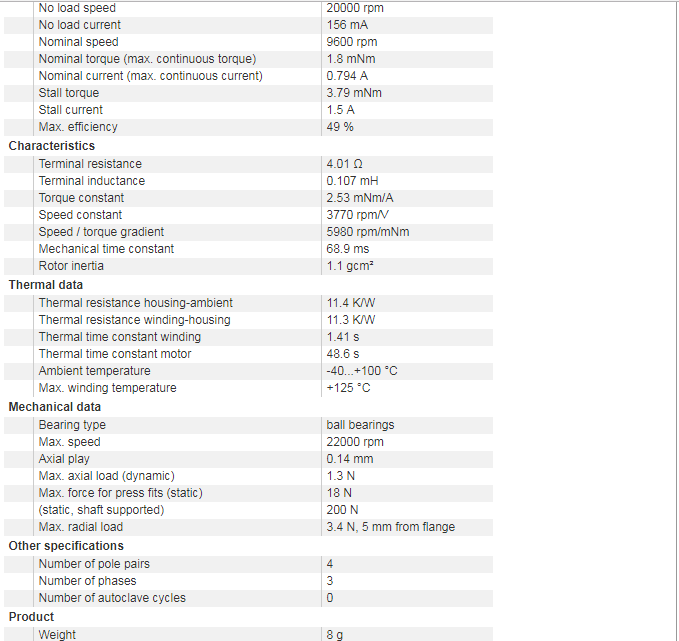
\includegraphics[width=0.7\linewidth]{figures/motorchar}
	\caption{ Flat motor $Ø$ 13.6 mm, brushless, 1.5 Watt, sensorless with 6V nominal voltage}
	\label{fig:323}
\end{figure}
%
%\begin{figure}[H]
%	\centering
%	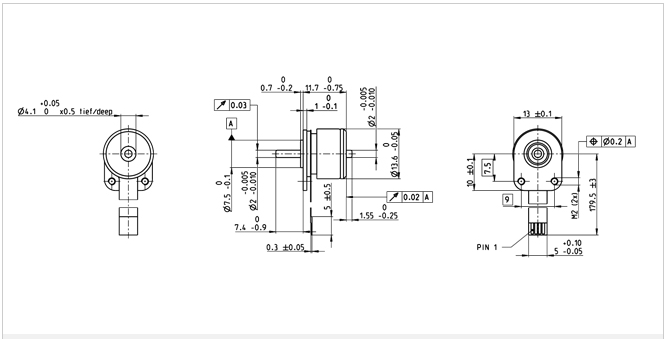
\includegraphics[width=0.7\linewidth]{figu%res/motor}
%	\caption{Motor technical illustration}
%	\label{fig:32}
%\end{figure}
%
Some of the torque in the mechanical part of the motors is used to overcome the friction and the rest is used in the motor shaft. An expression can be derived as
 \begin{equation*}
 T_{m} = T_{shaft} - T_{fric}
 \end{equation*}
  where $T_{m}$ is the nominal torque. Using the motor torque constant from the data sheet, $T_{fric}$ can be calculated as 
 \begin{equation*}
 T_{fric}	= k_{t}*I_{nom} - T_{m} 
 \end{equation*}    
where $I_{nom} $[A] is the nominal current. Viscous friction coefficient $b$ can now be calculated as
\begin{equation*}
	b	= \frac{T_{fric} }{\omega_{no-load}}
\end{equation*}
and $\omega_{no-load}$ is expressed in $rad/sec$. Finally, the back $emf$ constant is calculated as
\begin{equation*}
	k_{e}	= \frac{V_{nom} - I_{nom}R}{\omega_{no-load}}
\end{equation*}
where $V_{nom}$ is the nominal voltage and is equal to 6[V] and  $R$[Ohm] is the terminal resistance. 
\chapter{Derivation of the satellite equations of motion} \label{chap:C}
\textit{This section describes the derivation of the mathematical model of the satellite which contains the dynamic and kinematic model, based on the rigid body dynamics and kinematics.}
\subsection{Kinematic equation}
In this subsection, the focus will be on describing the orientation of the satellite. The method used for describing the satellite attitude is quaternion representation. It was decided to choose quaternion representation, because they provide a way to deal with singularities.

The quaternion $\textbf{q}(t)$ is defined as the attitude quaternion of a rigid body at time $t$ with respect to the inertial frame and at time $t+\Delta t$, the quaternion $\textbf{q}(t+\Delta t)$ is defined. The orientation quaternion can be divided into the quaternion at time $t$ and performing a quaternion multiplication with the rotation in the interval $\Delta t$ as follows:
\begin{flalign}
	\vec{ ^s_iq}(t+\Delta{t}) = \vec{ q}(\Delta {t}) \otimes \vec{ ^s_i q}(t) 
	\label{eq:qp}
\end{flalign}
where the orientation quaternion $	\vec{ ^s_iq}(t+\Delta{t}) $ represents the rotation of the spacecraft body frame with respect to the inertial frame

The quaternion at time $\Delta t$ can be express using the triad $u, v, w$, that represent the axis of the spacecraft as:
%
\begin{flalign}
	q_{1}(\Delta {t})  = {e_{u}\sin\frac{\Delta\Phi}{2}}
	\label{eq:q11}
\end{flalign}
%
\begin{flalign}
	q_{2}(\Delta {t}) = {e_{v}\sin\frac{\Delta\Phi}{2}}
	\label{eq:q2}
\end{flalign}
%
\begin{flalign}
	q_{3} (\Delta {t})= {e_{w}\sin\frac{\Delta\Phi}{2}}
	\label{eq:q3}
\end{flalign}
%
\begin{flalign}
	q_{4}(\Delta {t}) = {\cos\frac{\Delta\Phi}{2}}
	\label{eq:q4}
\end{flalign}
where $\Delta \Phi$ is the rotation at time $\Delta t$ and $e_u,e_v, e_w$ are the components along the triad $u, v, w$ at time $\Delta t$.

Using equation \ref{eq:q11} and equation \ref{eq:q4} and insert them into equation \ref{eq:qp} which yields:
\begin{flalign}
	\vec{ ^s_i q}(t+\Delta{t})
	= 
	\left\{\cos\frac{\Delta\Phi}{2} \underline I_{(4\times4)}+\sin\frac{\Delta\Phi}{2}
	\begin{bmatrix}
		0 &e_{z}&-e_{y}&e_{x} \\
		-e_{z}&0&e_{x}&e_{y}  \\ 
		e_{y}&-e_{x}&0&e_{z} \\
		-e_{x} &e_{y}&-e_{z}&0
	\end{bmatrix} 
	\right \} \vec{ ^s_i q}(t)
	\label{eq:quatm}
\end{flalign}  
%
where $\underline I$ is the identity matrix with the dimensions of $4\times4$.

In order to turn equation \ref{eq:quatm} into a differential equation, a small angle approximation it is used: 
\begin{flalign}
	&\Delta \phi = \omega \ \Delta t \\
	&\cos\frac{\Delta\Phi}{2} \approx 1 \\	
	&\sin\frac{\Delta\Phi}{2} \approx \frac{\omega \Delta t }{2} \\
	\label{eq:aprox}
\end{flalign} 
After using the approximation and substitute the terms into \ref{eq:quatm}, the following equation is obtained:
\begin{flalign}
	\vec{^s_i q(t+\Delta{t})} \approx \left[1 + \frac{1}{2} \underline \Omega \Delta(t)\right]\vec{^s_i q(t)}
	\label{eq:quatfinal}
\end{flalign} 
where $\underline \Omega$ is the skew symmetric matrix written in form:
\begin{flalign}
	\underline \Omega
	= 
	\begin{bmatrix}
		0& \omega_{w}& - \omega_{v}& \omega_{u} \\
		-\omega_{w}& 0&\omega_{u}& \omega_{v}  \\ 
		\omega_{v}& -\omega_{u}&0& \omega_{w} \\
		-\omega_{u}& -\omega_{v}& -\omega_{w}&0
	\end{bmatrix} 
	\label{eq:sm}
\end{flalign}
where the terms $\omega_u, \omega_v, \omega_w$ are the angular velocities components.

The rate of change in the orientation of the spacecraft $\vec{^s_i q(t)}$  can be found:
\begin{flalign}
	\vec{ ^s_i\dot q(t)} = \lim_{\Delta t\to 0} \frac{\vec q(t+\Delta t) - \vec q(t)}{\Delta t} = \dfrac{1}{2} \underline \Omega \  \vec{^s_i q(t)}
	\label{eq:finaleq}
\end{flalign} 

\subsection{ Dynamic equation}
The satellite dynamics are described using Euler's equation of motion and Newton's laws of motion. 
Using Euler's equation of motion, the relation between the change in angular momentum and the torques that affect the satellite is given as follows:
\begin{flalign}
	\vec{ \dot h} = \vec{N_{ext}} =  \vec{N_{mt}}+ \vec{N_{dist}}
	\label{eq:ec2}
\end{flalign} 
where $h$ is the angular momentum of a rigid body, $N_{ext}$ represent all the external torques that influence the satellite, $N_{mt}$ is the torque from the magnetorquers and $N_{dist}$ is the torque from the disturbances.

The change in angular momentum of the satellite can be express as the product between the angular acceleration and the moment of inertia:
\begin{flalign}
	{\vec{\dot h_{sat}}} = {\underline I_{s}}{\vec{\dot \omega}}
	\label{eq:ec3}
\end{flalign} 
where $h_{sat}$ is the angular momentum of the satellite, $\underline I_{s}$ is the moment of inertia of the satellite and $\vec{\omega}$ is the angular velocity.

Including the momentum wheels, the total angular momentum is given by:
\begin{flalign}
	{\vec{h_{tot}}} = \vec{h_{sat}} + \vec{h_{rw}}
	\label{eq:ec4}
\end{flalign} 
where $\vec{h_{rw}}$ is the angular momentum of the reaction wheels.
Therefore, the total angular momentum is described by:
\begin{flalign}
	{\vec{h_{tot}}} = {\underline I_{s}}{\vec{\omega}}+{\vec{h_{rw}}}
	\label{eq:ec5}
\end{flalign}
By rearranging terms, equation \ref{eq:ec5} becomes:
\begin{flalign}
	{\vec{\omega}} = {\underline I_{s}^{-1}} ({\vec{h_{tot}}}-{\vec{h_{rw}}})
	\label{eq:ec6}
\end{flalign}

Using Euler's equation of motion, the time derivative of $\vec{h_{tot}}$ expressed in the SBRF frame is:
\begin{flalign}
	&	\vec{ \dot h_{tot}} = \vec{ \dot h_{sat}} + \vec \omega \times \vec h_{tot}= \vec{  N_{mt}} + \vec{  N_{dist}} \\
	&\underline I_s {\vec{\dot{\omega}}} + \vec {\dot{h}_{rw}}+ \vec \omega \times \vec h_{tot} = \vec{  N_{mt}} + \vec{  N_{dist}} 
	\label{eq:ec7}
\end{flalign}
Subsequently, the angular velocity is separated and expressed as:
\begin{flalign}
	{\vec{\dot{\omega}}} = -\underline I_s ^{-1} \vec \omega \times \vec h_{tot} -\underline I_s ^{-1} \vec {\dot{h}_{rw}} + \underline I_s ^{-1}(\vec{  N_{mt}} + \vec{  N_{dist}}) 
	\label{eq:ec8}
\end{flalign}
Next, by replacing the cross product with a skew-symmetric matrix ${\underline S(\vec \omega)}$, \eqref{eq:ec8} becomes:
\begin{flalign}&{\vec{\dot{\omega}}}={-\underline I_{s}^{-1}\underline S(\vec \omega)\underline I_{s}\vec \omega-\underline I_{s}^{-1}\underline S(\vec \omega)\vec h_{rw}-\underline I_s ^{-1}\vec{  N_{rw}} + \underline I_s ^{-1}(\vec{  N_{mt}} + \vec{  N_{dist}})}
	\label{eq:ec9}
\end{flalign}
where $N_{mt}$ is the torque from the magnetorquers, $N_{rw}$ is the torque from the momentum wheels and the skew-symmetric matrix is:
\begin{flalign}
	{\underline S(\vec \omega)}
	\overset{\Delta}{=}
	\begin{bmatrix}
		0& -\omega_{3}& \omega_{2} \\
		\omega_{3}& 0&-\omega_{1}  \\ 
		-\omega_{2} & \omega_{1} &0
	\end{bmatrix} 
	\label{eq:skewsymmetricmatrix}
\end{flalign}
Moreover, the torque set to the momentum wheels is equal to the time derivative of the angular momentum:
\begin{flalign}
	\vec {N_{rw}} =  {\vec{ \dot{h}_{rw}}}
	\label{eq:ec10}
\end{flalign}
\subsection{Linearization of satellite  equations}
Due to the non-linear equations of motion of the satellite derived in the above sections, a linearization of these equations around an operating point is made, which will serve for designing a linear controller. 
\subsubsection{Kinematic  equation}
Starting with the non-linear kinematic equation which is given by:
\begin{flalign}
	\vec{ \dot q(t)} = \dfrac{1}{2} \underline \Omega   \vec{ q(t)}
	\label{eq:lke}
\end{flalign} 
Consequently, the quaternion can be expressed in a different form by dividing the initial quaternion $\vec{ q(t)} $ into a quaternion that represents the operating point and a quaternion error which represent a variation around the operating point:
\begin{flalign}
	\vec{ q}(t+\Delta{t}) = \vec{ q}(\Delta {t}) \otimes \vec{ q}(t) = \vec{ \bar{q}} \otimes \vec{\tilde{q}} 
	\label{eq:qpf}
\end{flalign}
where, \\
$\vec{ \bar{q}}$ is the operating point \\
$\vec{ \tilde{q}}$ is the quaternion error

By applying quaternion properties, the quaternion error can be written as:
\begin{flalign}
   \vec{\tilde{q}} = \vec{  \bar{q}}^{-1} \otimes \vec{ q} = \vec{  \bar{q}}^{\ast} \otimes \vec{ q}
	\label{eq:smallsignal}
\end{flalign}
where $ \vec{ {q}}^{-1} = \vec{q^{\ast}}$

Equation \ref{eq:lke} can be expanded by using a two quaternion multiplication, where the properties of these multiplication can be seen in appendix \ref{chap:B}, therefore equation \ref{eq:lke} becomes:
\begin{flalign}
\vec{ \dot q} = \dfrac{1}{2}  \vec{q} \otimes  \vec{q_{\omega}}
\label{eq:lkfe}
\end{flalign}
where $\vec{q_{\omega}}$ is the angular velocity quaternion and is given by: $\vec{q_{\omega}} = \vec{  \bar{q}} + \vec{  \tilde{q}}$

Taking the time derivative of equation \ref{eq:smallsignal} and using the product rule, the equation becomes:
\begin{flalign}
	\vec{\dot {\tilde{ q}}} = \vec{ \dot { \bar{q}}^{\ast}} \otimes \vec{ q} + \vec{   \bar{q}^{\ast}} \otimes \vec{\dot q}
	\label{eq:smallsignalr}
\end{flalign}
Inserting equation \ref{eq:lkfe} into equation \ref{eq:smallsignalr} and using the following properties of quaternions $\vec{q^{\ast}_{\omega}} = -\vec{q_{\omega}}$ and $(\vec q \vec{q_{\omega}}^{\ast}) = \vec{q^{\ast}_{\omega}} \vec{q^{\ast}} $, the equation \ref{eq:lkfe} result in:
\begin{flalign}
\vec{\dot {\tilde{ q}}} = \dfrac{1}{2} \Big [- \vec{\bar q_{\omega}} \otimes \vec{\tilde{q}} + \vec{\tilde{q}} \otimes \vec{\bar q_{\omega}} + \vec{\tilde q} \otimes \vec{\tilde q_{\omega}} \Big ]
\label{eq:smallsignfalr}
\end{flalign}
In order to express the products quaternion from the previous equation, the product of these quaternion can be written as a matrix that have the real and the complex part and one quaternion, which will end up as a product between a matrix and a vector. Therefore, the product quaternion between $\vec{\bar q_{\omega}} \otimes \vec{\tilde{q}} $ can be rewritten as:
\begin{flalign}   
\vec{\bar q_{\omega}} \otimes \vec{\tilde{q}}  
= 
\begin{bmatrix}
& - \underline S(\vec{\tilde q}) + \underline{\vec 1} {\tilde q_4} & \vec{\tilde q} \\
& - \vec{\tilde q}^\mathsf{T}& {\tilde q_4}  \\ 
\end{bmatrix} 
\begin{bmatrix}
&   \vec{\bar \omega} \\
& 0 \\ 
\end{bmatrix} 
=
\begin{bmatrix}
& - \underline S(\vec{\bar \omega}) \vec{\tilde q} + \underline{\vec 1} {\tilde q_4} \vec{\bar \omega}  \\
& - \vec{\tilde q}^\mathsf{T} \vec{\bar \omega}\\ 
\end{bmatrix} 
\label{eq:sffm}
\end{flalign}
where the following property is used $\underline S(\vec{\bar \omega}) \vec{\tilde q} = - \underline S(\vec{\tilde q} ) \vec{\bar \omega} $ and $ S(\vec \omega)$ is the skew symmetric matrix.

Similarly, the product quaternion between $ \vec{\tilde{q}} \otimes \vec{\bar q_{\omega}}  $ is found:
\begin{flalign}   
\vec{\tilde{q}} \otimes \vec{\bar q_{\omega}}  
= 
\begin{bmatrix}
& - \underline S(\vec{\bar \omega}) & \vec{\bar \omega}\\
& - \vec{\bar \omega}^\mathsf{T}& 0  \\ 
\end{bmatrix} 
\begin{bmatrix}
&  \vec{\tilde{q}} \\
&  {\tilde q_4}\\ 
\end{bmatrix} 
=
\begin{bmatrix}
& - \underline S(\vec{\bar \omega}) \vec{\tilde q} +  \vec{\bar \omega} {\tilde q_4}   \\
& - \vec{\tilde \omega}^\mathsf{T} \vec{\tilde q}\\ 
\end{bmatrix} 
\label{eq:sfm}
\end{flalign}
The last product quaternion can be found in the same manner:
\begin{flalign}   
	\vec{\tilde{q}} \otimes \vec{\tilde q_{\omega}}  
	= 
	\begin{bmatrix}
		& - \underline S(\vec{\tilde \omega}) & \vec{\tilde \omega}\\
		& - \vec{\tilde \omega}^\mathsf{T}& 0  \\ 
	\end{bmatrix} 
	\begin{bmatrix}
		&  \vec{\tilde{q}} \\
		&  {\tilde q_4}\\ 
	\end{bmatrix} 
	=
	\begin{bmatrix}
		& - \underline S(\vec{\tilde \omega}) \vec{\tilde q} +  \vec{\tilde \omega} {\tilde q_4}   \\
		& - \vec{\tilde \omega}^\mathsf{T} \vec{\tilde q}\\ 
	\end{bmatrix} 
	\label{eq:sfgfm}
\end{flalign}
Using the following property, a small approximation for the angle is made %Satellite Attitude Control Using Only Electromagnetic Actuation/ rafal%:
\begin{equation}
	  \lim_{\theta \to 0} \vec q = 	  \lim_{\theta \to 0} 
	 \left[ 
	 \begin{array}{cccc}
	 	\vec q \\
	 	q_4 
	 \end{array}
	 \right] 
	 =  \lim_{\theta \to 0} 
	 \left[ 
	 \begin{array}{cccc}
	    e_u \sin (\tfrac{\theta}{2}) \\
	 	e_v \sin (\tfrac{\theta}{2}) \\
	 	e_w \sin (\tfrac{\theta}{2}) \\
	 	\cos (\tfrac{\theta}{2}) 
	 \end{array}
	 \right] 
\end{equation}
where $\vec{\tilde q} \rightarrow $ 0 and $\tilde q_4 \rightarrow $ 1

Therefore, equation \ref{eq:sfgfm} can be rewritten by using this property as:
\begin{flalign}   
	\vec{\tilde{q}} \otimes \vec{\tilde q_{\omega}}  
	=
	\begin{bmatrix}
		& - \underline S(\vec{\tilde \omega}) \vec{\tilde q} +  \vec{\tilde \omega} {\tilde q_4}   \\
		& - \vec{\tilde \omega}^\mathsf{T} \vec{\tilde q}\\ 
	\end{bmatrix} 
=
\vec{\tilde q_{\omega}}  
	\label{eq:sfgffm}
\end{flalign}
Collecting terms and inserting equation \ref{eq:sffm},  \ref{eq:sfm}, \ref{eq:sfgffm} into equation  \ref{eq:smallsignfalr} yields the following form:
\begin{flalign}
	\vec{\dot {\tilde{ q}}} \approx  
	- \frac{1}{2}
	\begin{bmatrix}
		- \underline S(\vec{\bar \omega}) \vec{\tilde q} + \underline{\vec 1} {\tilde q_4} \vec{\bar \omega}  \\
		- \vec{\tilde q}^\mathsf{T} \vec{\bar \omega}\\ 
	\end{bmatrix} 
+ \frac{1}{2}
\begin{bmatrix}
	- \underline S(\vec{\bar \omega}) \vec{\tilde q} +  \vec{\bar \omega} {\tilde q_4}   \\
    - \vec{\tilde \omega}^\mathsf{T} \vec{\tilde q}\\ 
\end{bmatrix} 
+\frac{1}{2} \vec{\tilde q_{\omega}} \approx
\begin{bmatrix}
	- \underline S(\vec{\bar \omega}) \\
	0\\ 
\end{bmatrix}
\vec{\tilde q} + \frac{1}{2} \vec{\tilde q_{\omega}}
	\label{eq:smallsignffalr}
\end{flalign}
\subsubsection{Dynamic  equation}
Next, the non-linear dynamic equation is given by:
\begin{align*}
	\begin{split}
	{\vec{\dot{\omega}}} &={-\underline I_{s}^{-1}\underline S(\vec \omega)\underline I_{s}\vec \omega-\underline I_{s}^{-1}\underline S(\vec \omega)\vec h_{rw}-\underline I_s ^{-1}\vec{  N_{rw}} + \underline I_s ^{-1}(\vec{  N_{mt}} + \vec{  N_{dist}})} = \\
	&= {\underline I_{s}^{-1}} [\vec{  N_{dist}} + \vec{  N_{ctrl}} - S(\vec \omega) (\underline I_{s}\vec \omega + \vec h_{rw})] 
\label{eq:ec34}
\end{split}
\end{align*}
An operating point is introduce as:
\begin{flalign}
    \vec{\omega} = \vec{\bar{\omega}} + \vec{\tilde{\omega}} 
	\label{eq:smallsi4gnal}
\end{flalign}
where the angular velocity $\vec{\omega}$ is separated into a operating point $\vec{\bar{\omega}}$ and the error around this operating point $\vec{\tilde{\omega}}$.

The next step is to use a a first order Taylor expansion for linearizing the time derivative of the angular velocity, with the mention of neglecting the $ \vec {  N_{dist}}$ which is assumed to be insignificant.
\begin{flalign}
		{\vec{\dot{\omega}}} \approx {-\underline I_{s}^{-1}} \frac{d {\vec{\dot{\omega}}}}{d {\vec{{\omega}}}} \Big|_{{\vec{{\omega}}} = {\vec{{\bar \omega}}}} \vec{{\tilde \omega}} -  {\underline I_{s}^{-1}} \frac{d {\vec{\dot{\omega}}}}{d {\vec{{h_{rw}}}}} \Big|_{{\vec{{h_{rw}}}} = {\vec{{\bar h_{rw}}}}} \vec{{\tilde h_{rw}}} + {\underline I_{s}^{-1}} \frac{d {\vec{\dot{\omega}}}}{d {\vec{{N_{ctrl}}}}} \Big|_{{\vec{{N_{ctrl}}}} = {\vec{{\bar N_{ctrl}}}}} \vec{{\tilde N_{ctrl}}} 
		\label{eq:ec3f4}
\end{flalign}
By using the property $\underline S(\vec \omega)\underline I_{s}\vec{\bar \omega} = - \underline S(\underline I_{s}\vec{\bar \omega}) \vec \omega$ and rewriting the \ref{eq:ec3f4} by expanding the terms, will result the linearized dynamic equation:
\begin{flalign}
{\vec{\dot{\omega}}} = \underline I_{s}[ \underline S(\underline I_{s}\vec{\bar \omega}) - \underline S(\vec{\bar \omega})\underline I_{s} + \underline S(\vec{\bar h_{rw}}) ] {\vec{\tilde{\omega}}} - \underline I_{s} \underline S(\vec{\bar \omega}) \vec{\tilde h_{rw}} + \underline I_{s}  \vec{\tilde N_{ctrl}}
\label{eq:ec3fr4}
\end{flalign}

\chapter{Maximum Torque Demand} \label{chap:D}

In order to be able to choose actuators that are able to satisfy the control demands, the maximum torque demand for Earth station tracking needs to be calculated. As a first step, the maximum angular acceleration is calculated for a scenario where the satellite always points towards the Earth station. Figure \ref{fig:maxOmega} shows the angular velocity of the satellite orbiting at 600 km on a circular orbit, while the station is at sea level. When the satellite is closest to the Earth station, the station is on the nadir of the satellite. The angular velocity is the highest when the satellite flies above the station. Since it is an extremum, the angular acceleration in that instant is zero. By differentiating the angular velocity, the angular acceleration shown in Figure \ref{fig:maxOmegaDot}. The maximum value of angular acceleration is $1.085 \times 10^{-4} \frac{rad}{s^2}$. 

If the satellite is rotating around its principal axis of inertia with the highest value, $0.0022 k\!g \, m^2$, the maximum angular acceleration demands  \boldmath$ 2.388 \times 10^{-7} Nm$.


\begin{figure}[H]
	\begin{subfigure}{0.5\linewidth}
			\centering
		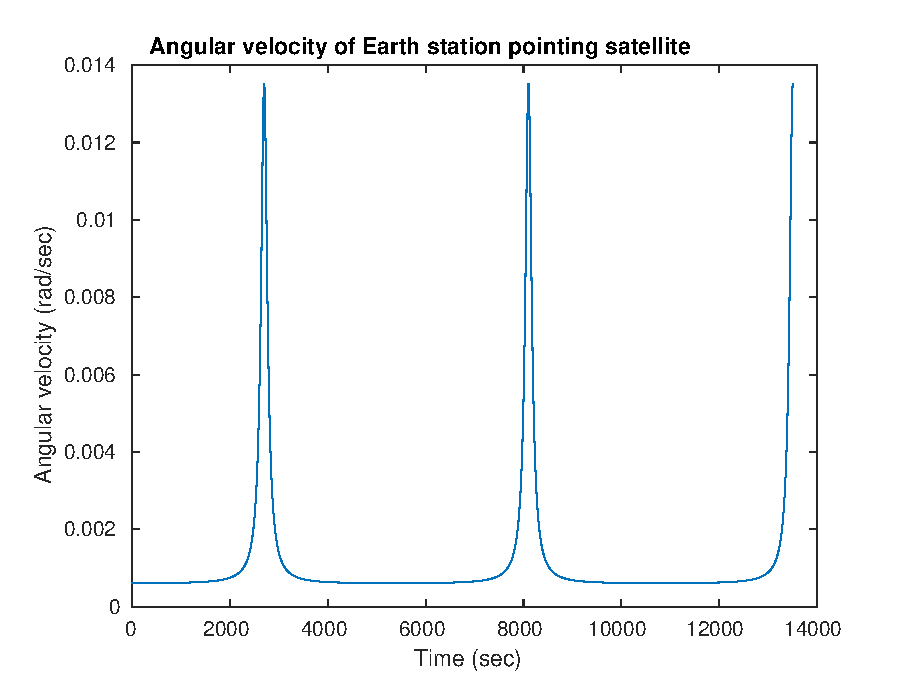
\includegraphics[width=80mm]{figures/maxOmega}
		\caption{Angular Velocity of Earth station pointing satellites.}
		\label{fig:maxOmega}
	\end{subfigure}
	\begin{subfigure}{0.5\linewidth}
	\centering
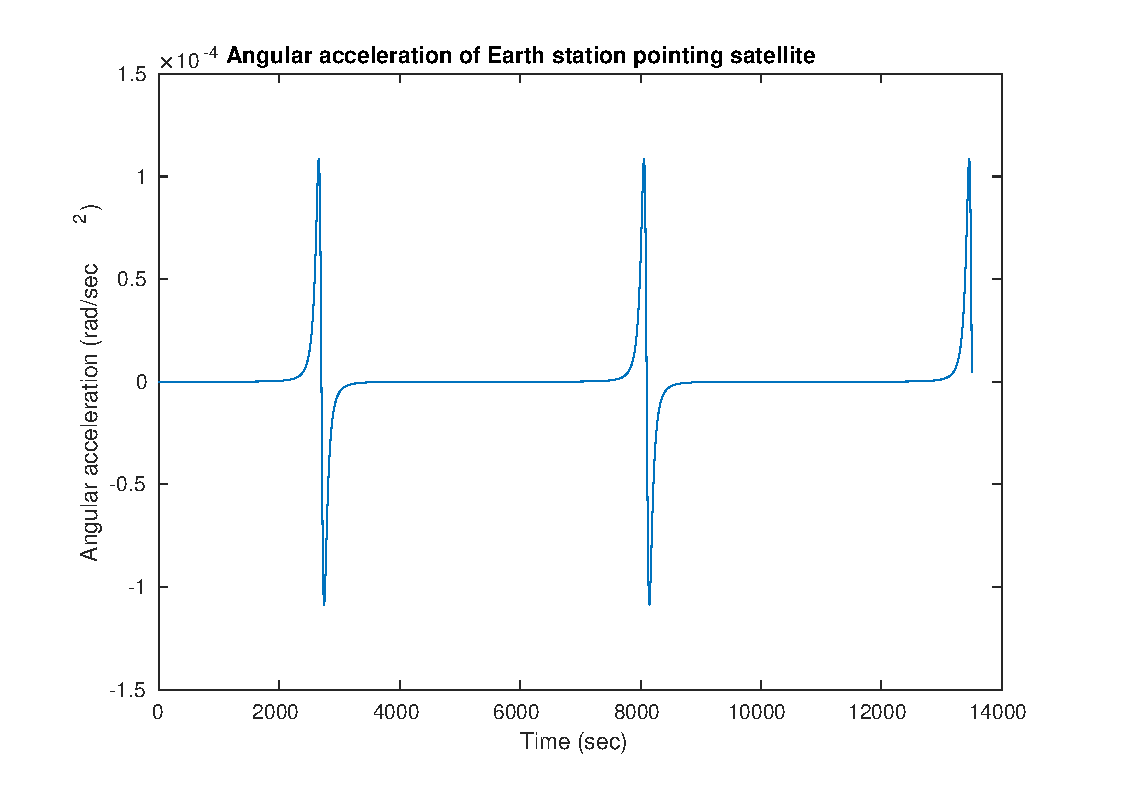
\includegraphics[width=80mm]{figures/maxOmegaDot}
\caption{Angular Acceleration of Earth station pointing satellites.}
\label{fig:maxOmegaDot}
\end{subfigure}
\end{figure} 

\chapter{Alternative method for identifying reaction wheel fault}

With enough computational power the faulty reaction wheel can be detected through the calculated reaction wheel output torque, assuming only one reaction wheel is faulty. It is done by calculating the difference between 3D torque demand and actual 3D torque output. 

\begin{equation}
\vec{N}_{rw} = \underline{I}_s \dot{\vec{\omega}}  + \vec{\omega} \times \vec{h_{rw}} - \vec{N_{mt}} - \vec{N_{dist}}
\end{equation}

Then the difference between torque demand and torque output is calculated. The reaction wheel that has the most similar axis orientation to the torque difference is deemed as faulty.

\begin{equation}
\vec{N}_{rw}^{d} - \vec{N}_{rw} = 
\vec{N}_{rw}^{diff}
\end{equation}

\begin{equation}
 \pm \vec{N}_{rw}^{diff}  \stackrel{?}{\approx} \vec{axis} 
\end{equation}

If the torque error exceeds a certain threshold, then the faulty wheel index can be identified as

unit vectors!!!

\begin{equation}
faultyWheelIndex = \arg\min_i ( \pm \vec{N}_{rw}^{diff} - \vec{axis}_i ) 
\end{equation}

\todo{mention unit vector notation, decide notation for axis, express axis according to q}

Note: the lag for torque change and wheel saturation has to be taken into account separately, as those don't count as faults. 
Thresholds should be applied.


\printbibliography

%

%%% List of Corrections
%\listoffixmes\documentclass[options]{class}

\end{document}
